\documentclass[a4paper, 12pt]{report}
\usepackage{times}

\usepackage[leftcaption]{sidecap}
\usepackage{subfigure} % figures can have sub chunks
\usepackage{geometry} % this maxes page usage, making the below unnecessary
\textwidth = 6.75in
\oddsidemargin = -0.25in
\textheight = 10in
\topmargin = -0.5in
\headheight = 15pt
\usepackage{fancyhdr}
\usepackage{pdfpages}

%highlighting
\usepackage{color}

% accents in listings
%\usepackage[utf8]{inputenc}
%\usepackage{listingsutf8}

% Japanese
\usepackage{CJKutf8}

% for textnumero symbol
\usepackage{textcomp}

% sideways tables
\usepackage{rotating}

% longtable tabularx
\usepackage{ltxtable}
\usepackage{array}
\usepackage{longtable}

% list spacing
\usepackage{enumitem}
\setlist{nolistsep}
\setlist{noitemsep}
% paragraph spacing
\setlength{\parskip}{0.5em}
\setlength{\parindent}{0cm}

% table width control
\usepackage{tabularx}

% captions in minipage
\usepackage{caption}

% float barrier
\usepackage[section]{placeins}

% multi-page figure type
\usepackage{listings}

\pagestyle{fancy}
\lhead{{\it Alex Birch}}
\chead{ChibiPoint: Accessible Pointing for Web Applications}
\rhead{}
\lfoot{}
\cfoot{\thepage}
\rfoot{}

% for capitals font in signature
\usepackage[T1]{fontenc}

\usepackage{amsmath}

% For figures
\usepackage{graphicx}
\DeclareGraphicsExtensions{.pdf,.png,.jpg}
\usepackage{float}

%,bibencoding=utf8
\usepackage[sorting=none,backend=bibtex]{biblatex}
%\usepackage[sorting=none,backend=biber,bibencoding=utf8]{biblatex}
\bibliography{Diss}

\usepackage[colorlinks]{hyperref}
\usepackage[noabbrev]{cleveref}
\crefformat{section}{section #2#1#3}
\crefdefaultlabelformat{[#2#1#3]}

\usepackage[nomain,acronym,toc,section,numberedsection=autolabel]{glossaries} % make a separate list of acronyms
%\makeindex
\makeglossaries

\title{ChibiPoint: Accessible Pointing for Web Applications}
\author{Alexander Birch}
\date{\today}
\begin{document}
\newglossaryentry{computer}
{
  name=computer,
  description={is a programmable machine that receives input,
               stores and manipulates data, and provides
               output in a useful format}
}


%\newacronym[\glsshortpluralkey=cas,\glslongpluralkey=contrived
%acronyms]{aca}{aca}{a contrived acronym}

\newacronym{rsi}{RSI}{Repetitive Strain Injury}
\newacronym{gui}{GUI}{Graphical User Interface}
\newacronym{w3c}{W3C}{World Wide Web Consortium}
\newacronym{wai}{WAI}{Web Accessibility Initiative}
\newacronym{wcag}{WCAG}{Web Content Accessibility Guidelines}
\newacronym{socog}{SOCOG}{The Sydney Organizing Committee for the Olympic Games}
\newacronym{cthdda}{Cth DDA}{Commonwealth Disability Discrimination Act 1992}
\newacronym{goms}{GOMS}{Goals, Operators, Methods, and Selection rules}

\newglossaryentry{accesskeys}
{
  name=access keys,
  description={a means for users to travel between distant or unrelated interface components using keyboard shortcuts}
}

\newglossaryentry{keybinding}
{
  name=key binding,
  plural=key bindings,
  description={mapping of keys, or combinations thereof, to actions}
}

\newglossaryentry{browserextension}
{
  name=web browser extension,
  description={(in the context of the Google Chrome web browser): extensions are small software programs that can modify and enhance the functionality of the Chrome browser. You write them using web technologies such as HTML, JavaScript, and CSS.}
}

\newglossaryentry{browsingcontext}
{
  name=browsing context,
  description={a window or tab in a web browser that hosts a webpage}
}
\maketitle
%\newpage
\begin{abstract}
[Revisit this once Results section is finalized, and once Conclusions section is written]
\end{abstract}

\tableofcontents
%\pagebreak

%\chapter*{Introduction}

\chapter{Introduction}

\section{Context and Motivation}
Software is moving to the web. We now rely on `web applications' for services such as shopping, banking, and social networking.

Many of these websites are designed to be used with mice, or equivalent pointing devices (such as touchscreens).

Many users cannot use mice to point in websites, due to input restrictions:
\begin{enumerate}
\item Some users are too disabled (due to conditions like \gls{rsi}) to use the input device provided to them
\item More suitable input hardware, such as bespoke accessibility hardware, can be hard to prescribe (due to lack of knowledge, or access to a needs assessor) or procure (due to rarity or expense)
\item Some devices (such as Smart TVs or games consoles) inherently enforce a standard, limited, input hardware (such as a remote or gamepad) in stead of a better pointing device
\end{enumerate}

Such users are denied full access to a web that relies on a robust pointing mechanism.

Attempts have been made to push a standard for mouseless navigation on the web: tabbing navigation. Unfortunately this mechanism is ineffective, unpredictable and inefficient.

It is challenging to optimise websites to accommodate tabbing navigation. In practice the web remains inaccessible, despite the availability of standards for accessible development.

\textit{A more detailed background is disclosed in \Cref{chap:context}.}
\section{Literature \& Technology Review}
We confirm here the need for an alternative pointing mechanim, and explore the approaches that have been attempted already.

We review what factors exist in designing for accessible keyboard control. We assess the state of keyboard accessibility, in general and for the web. We explore also general web accessibility, and how the problem it presents has been addressed up until now. We explore the vectors through which accessibility can be added to the web. We ascertain whether there exist any novel approaches to keyboard pointing. We review whether accessibility standards are capable of solving the problem of keyboard pointing in the web, and finally look for experimental methods to evaluate the performance of keyboard pointing systems.

We conclude that the root of the problem is that standards push a navigation mechanism that is not suited to the task of pointing. We decide that a new mechanism could be delivered in the form of a web browser extension.
% The deliverable for this dissertation is anticipated to be a browser extension that adds accessibility onto web content, favouring a novel interaction approach over the experience prescribed as accessible by web standards.

% The key points to explore are:
% \begin{itemize}
% \item What factors exist in accessible design for keyboard usage, in general and for the web?
% \item Have approaches to keyboard accessibility evolved over time?
% \item Has the status of keyboard accessibility evolved over time?
% \item Does literature support the notion that `keyboard accessibility in the web is generally lacking'?
% \item Does work exist around making web content more accessible for the keyboard?
% \begin{itemize}
% \item Has web accessibility changed over time?
% \item Does work exist around adding extra accessibility to web content without the web developer's involvement?
% \begin{itemize}
% \item Does this work aim to bring content in line with a suggested web standard, or is a novel approach preferred?
% \end{itemize}
% \item Does work exist around adding extra accessibility to web content via the user agent?
% \end{itemize}
% \item Do there exist any novel keyboard pointing methods?
% \item Is there any support for the notion that web accessibility standards prescribe a sub-par experience?
% \item Are there any experimental techniques that are recruited for evaluating task performance on keyboards?
% \begin{itemize}
% \item Are there any comparisons with mouse performance?
% \end{itemize}
% \end{itemize}
% SUMMARY of literature review
\section{Problem statement and Hypotheses}
\subsection{Problem statement}
Existing work focuses around making websites conform to accessibility standards. Yet even using tabbing navigation within a tab-accessible website is not an ideal browsing experience.

The pointing mechanism provided by `tabbing navigation' is inherently limited, so \textbf{a more suitable mouseless pointing mechanism needs to be developed: one that is designed to cope with real websites, rather than idealized ones.}

To solve mouseless pointing on a wide variety of input hardware, a mechanism is required that maps well to that wide variety of input hardware. One that is effective, predictable and efficient.
%Many input devices generate input which can be parsed as discrete symbols; for example gestures or speech samples. A keyboard-based proof-of-concept could be mapped to work with symbols

\subsection{Hypotheses}
\label{chap:hypotheses}
We believe that our keyboard navigation system for the web, ChibiPoint, provides an improved mechanism for pointing as compared to tabbing.

\newcommand{\hypone}{Hypothesis 1: ChibiPoint is generally more efficient at web navigation than tabbing}
\subsubsection{\hypone}
We hypothesise that our system, \textbf{ChibiPoint, requires significantly fewer keypresses to navigate webpages, than does `tabbing navigation'} (the current standards-prescribed method for keyboard navigation).
`Navigate webpages' is a broad term, as there are many classes of pointing that need to be analysed. The more detailed hypothesis is that, \textbf{given several distinct classes of pointing, ChibiPoint requires fewer (or equal) keypresses, for a large majority (>80\%) of these scenarios}. Since we analyse two versions of ChibiPoint, it should be understood that we require at least one of these to outperform tabbing in a majority of tasks.

\newcommand{\hyptwo}{Hypothesis 2: ChibiPoint's `flyouts' feature, reduces further the required keypresses for web navigation}
\subsubsection{\hyptwo}
We hypothesise that the novel `flyouts' feature of ChibiPoint, which assigns hotkeys to suggested buttons on the webpage, contributes to reducing the number of keypresses required by ChibiPoint for web navigation, compared to using just its standard pointing method of hierarchically drilling through the page and pointing at elements using crosshairs.
In other words, we hypothesise that ChibiPoint `with crosshairs and flyouts enabled' performs a large majority (>80\%) of pointing scenarios in fewer keypresses than ChibiPoint `with just crosshairs enabled'.

% Concise statement of problem
% State efficiency goal
\section{Goals and Methods}
% What we intend to solve, and how
\subsection{Goals}
We intend to demonstrate that a more effective, efficient, and predictable mouseless pointing mechanism than `tabbing navigation' can be made for the web. The mechanism needs to be capable of achieving widespread availability --- across many browsers and input systems.

The input mechanism used by the web browser extension should be input hardware-agnostic: that is, it must accept as input a language that can be mapped to by a wide variety of input methods.

\subsection{Methods}
\subsubsection{Deliverable}
We will produce a proof-of-concept web browser extension (for Google Chrome), that provides mouseless pointing in a variety of real-world websites. The implementation will recruit only technologies that are available to all web browsers (i.e. HTML5, CSS and Javascript). This foundation enables it inherently to be completely cross-platform and cross-browser. Any external libraries used must be free in cost, so as not to impose a price barrier to availability.

\subsubsection{Supported input}
The input language for the system will be an instance of symbol-based input: keystroke sequences. Thus a keyboard-based interface theoretically serves as a proof-of-concept for other input systems that can produce a vocabulary of discrete inputs, for example gestures or spoken words. The more limited this proof-of-concept's vocabulary is, the more devices it allows to map to its space.

\subsubsection{Qualitative difference}
\label{sec:qualitative_promises}
We aim to deliver the following qualitative improvements over `tabbing' navigation:
\begin{itemize}
\item We will improve upon the efficiency of tabbing navigation's linear trawl, by using a hierarchical traversal.

\begin{itemize}
\item We will solve tabbing navigation's effectiveness problems: we avoid falling into `focus traps' by avoiding a relative traversal.
\item We will solve the feedback problem represented by `lack of visual indicator of focus', by painting our own visual indicators on elements.
\end{itemize}

\item We will improve predictability of navigation by using a spatial traversal rather than tabbing navigation's markup-driven traversal.
\end{itemize}

\section{Results / Contributions}
Both our hypotheses are confirmed: ChibiPoint provides a significantly more efficient pointing mechanism than tabbing. The novel `flyouts' feature contributes further to ChibiPoint's efficiency.

We contribute a widely portable mechanism --- ChibiPoint recruits in its development only widely-available web technologies. The system is compatible with many `real-world' websites that expect mice. Some implementation bugs exist, and these are felt to be fixable.

ChibiPoint demonstrates a navigation mechanism whose input vocabulary is a simple symbol sequence. By showing an instance of its application with keyboard input, we imply that the mechanism is compatible also with other point systems that can produce symbol output, such as gesture control or speech. Thus its efficient navigation could be extended to other mouseless devices like Smart TVs.
% Summarise our most important findings
% Cast findings as contributions to research field

[Revisit this once Results section is finalized, and once Conclusions section is written]
\section{Thesis overview}
\newcommand{\chapterref}[2]{\Cref{#1}, \textit{#2},}
% Overview of remainder of thesis
The remainder of the thesis is composed as follows:

\chapterref{chap:context}{Detailed Context \& Motivation} discloses more detail around the background and motivation for this work.\\
\chapterref{chap:litreview}{Literature \& Technology Review} confirms the need for an alternative web pointing mechanism, and explores the approaches recommended, as well as reviewing what solutions have been attempted already.\\ %We review what factors exist in designing for accessible keyboard control.
\chapterref{chap:reqanddesign}{Requirements \& Design} details the design of our system and pointing mechanism.\\
\chapterref{chap:implementation}{Implementation} describes how we built our web browser extension.\\
\chapterref{chap:evaluation}{Evaluation} chronicles the output of a usability study and a larger quantitative study. We determine how our web browser extension compares to tabbing navigation, and determine also the contribution of our novel algorithm for suggesting `clickables'.\\
\chapterref{chap:conclusions}{Conclusions \& Future Work} discusses our contribution to the field, and ways to extend the work.

\chapter{Detailed Context \& Motivation}
\label{chap:context}
[@Fabio: this whole chapter is copypasta from the original Project Proposal. I've not proofread it, so cannot guarantee if it's consistent with the current problem I say I am trying to solve, or the solution I propose.]
\section{Problem}
\subsection{Problem Context}
Some domain knowledge will be divulged in this section, prior to describing the problem under investigation. Namely, the case for accessible navigation alternatives' necessity, and also the relevance of the web in contributing to the size of the problem.
\paragraph{Need for accessibility}
Computer users are not uniform in their capabilities and preferences. For this reason, users differ in the input mechanisms they choose for interacting with software. Some users may prefer to perform tasks using a keyboard rather than using a mouse, for example. Commonly mouse and keyboard will be recruited together. However some users' input strategies are constrained by factors such as disability: occupational syndromic conditions such as ~\gls{rsi} can preclude the ability to use a mouse, keyboard or both~\cite{trewin1999keyboard}. ~\gls{rsi} and related disabilities are growing in prevalence, representing by some estimates 22\% of people~\cite{rsiprevalence}. This disability accounts for one third of workers' compensation costs in the US private industry~\cite{barr2002pathophysiological}.

When the user cannot or will not use the primary input scheme of the software, it becomes necessary to provide alternative input modes. For simple interfaces that use standard components, keyboard and mouse can be both supported implicitly without additional development effort. Conversely, complex interfaces or ones involving non-standard components require explicit treatment from the developer to ensure that all funcitonality can be accessed. In cases where accessibility is not a priority or concern of the software developer, users can be left unable to use said software.

\paragraph{Rise of web applications}
Even as early as 2001, software made the leap to the web~\cite{ginige2001web}. Services such as email, banking and word processing are being produced as web applications, due to a few advantages:
\begin{itemize}
  \item high cross-platform, cross-device support \& penetration
  \item centralized maintenance and upgrade
  \item centralized storage of user data
  \item (consensual) monetization of user information, telemetry
  \item scalability (down and up)
  \item zero end-user installation
  \item redundancy
 % finish list if anyone cares
\end{itemize}
Email clients such as Outlook~\cite{outlookcom} benefit from this; emails can be accessed from any web-enabled device without any need for installation, all users can be kept on the latest version without effort on their part, and user data can be analyzed to improve content filters or provide relevant advertisement. At peak times of operation, more servers can be recruited, and vice-versa, such that the cost of operations can be finely controlled based on usage.
\subsection{Problem Description}
This transition away from native applications is leading to sacrifices in accessibility. Web applications run within a native application (the browser), so there is conflict when it comes to the following accessibility paradigms:
\begin{itemize}
 \item menu actions
 \item keyboard shortcuts
 \item tab order
 \item citizenship amongst other applications
\end{itemize}

Even on the conceptual level, there are problems with using the web to serve applications: a web application tries to fit a full application interface inside a web browser's (already saturated) interface. It is a second-class citizen; a user cannot `switch application' to it, only trawl for it amongst the tabs and windows of some web browser.

Additionally, web applications are often guilty of foregoing standard UI components in favour of a bespoke UI made in JavaScript or CSS. This can be used to deliver impressive effects like transitions, or serve complicated shapes of interactive content or buttons. But this freedom makes it all too easy to produce inaccessible elements, such as buttons that can't be pressed or focused using the keyboard.

\subsection{Existing Approaches}
There exist at present a few categories of solution to the problem of web accessibility:
\begin{itemize}
\item following web development guidelines to produce a standards-compliant website
\item using web technologies to create a non-standard interaction behaviour
\item making the web browser behave in a non-standard manner
\end{itemize}
\subsubsection{Recommended web practice}
\label{recommendedpracticesection}
Guidance is provided on how to develop accessible web applications, in the form of the \gls{w3c}'s \gls{wcag}~\cite{chisholm2001web}~\cite{wcag}. A description and analysis on its recommendations for keyboard access follows:
\paragraph{Pointing with access keys}
\label{accesskeysection}
  \Gls{accesskeys} are one paradigm used for keyboard accessibility in the HTML5 specification~\cite{html5specaccesskeys}. Hotkeys can be assigned for the focusing of interface elements, used in conjuction with modifier keys. This system allows the user to jump instantly between distant or unrelated interface elements. However, its usefulness is predicated on the discoverability and availability of said \glspl{keybinding}.

  It is hard to avoid conflicts with existing shortcuts used by the user's accessibility technologies, since there is no standardisation between browsers as to which modifier keys to use~\cite{webaimaccesskeys}. Recommendation exists that \gls{accesskeys} be avoided altogether for this reason. Another problem with \gls{accesskeys} is that they rely on explicit implementation by developers. They also require learning of a layout, and although attempts have been made at increasing standardisation~\cite{AccesskeyStandardisation}, that standardisation is not prevalent.
\paragraph{Making interface tab-accessible}
   It is difficult to develop a tab-accessible web application~\cite{watanabe2012using}. Since the only pointing expression assumed is the tab key, layout must be linearized. Not only is this hard to design and develop for (requiring explicit effort and markup changes), the end result is not that impressive; content that is far away in the tab order unavoidably requires repeated hammering of the tab key (making it far harder to reach with the keyboard than with a pointing device). Plus linearization doesn't suit web content, which often has navigation bars, side bars, feeds or some similar multi-dimensional layout.
\subparagraph{Short-circuiting tab journey with skip-links}
\label{sec:skiplinks}
  An exception to the content linearization problem is skip links, which can short-circuit the tab journey around a page by allowing the user to choose alternative insertion points. These again require effort and understanding from the developer. It is hard to provide a suitable set of skip links, and again the best case is still a hamfisted pointing experience, where the user can't predict where they are going to or from.
\paragraph{Conclusion}
  Even a website designed with accessibility standards in mind can be quite hard to navigate; web standards prescribe only a very limited amount of keyboard expression, so meeting these provides a very limited experience.

\subsubsection{Using web technologies to augment accessibility}
  Whilst it is possible (to an extent) to create \glspl{keybinding} in web content (through access keys \cref{accesskeysection}, or through JavaScript event libraries like MouseTrap~\cite{Mousetrap}), for the most part web applications do not make use of this. Possible reasons for this are:

\begin{itemize}
 \item no agreed standard exists for how websites should provide keyboard shortcuts
 \item web application shortcuts are likely to conflict with native application's shortcuts
 \item existing native application shortcuts are hard to tiptoe around, since any browser or extensions could be used
 \item some devices (for example smartphones) do not have the same expressive keyboard capability
 \item would only be available on those websites that chose to implement it
 \item websites not guaranteed to implement in a uniform way
\end{itemize}

\subsubsection{Changing the web browser}
\label{changingwebbrowser}
Adding accessibility on top of web content can be achieved through a \gls{browserextension}. This can change the way content is treated so as to work better for the preferred input mode. In some implementations, the browser is extended through the use of web technologies, which can coexist with the content of the website.
One such example is Type-Ahead-Find~\cite{typeaheadfind}, which allows users to move keyboard focus to hyperlinks by typing the content of said hyperlink. Another example is Stylish~\cite{stylish}, which allows users to redesign a website to suit their needs.

\Glspl{browserextension} solve some of the problems associated with using web technologies alone to augment accessibility: \glspl{keybinding} are uniform across the user's browsing experience, so a user can configure non-conflicting shortcuts. The solution is also easy to distribute via \gls{browserextension} repositories.
\section{Proposed Solution}
[@Fabio: (again) this whole chapter is copypasta from the original Project Proposal. I've not proofread it, so cannot guarantee if it's consistent with the current problem I say I am trying to solve, or the solution I propose.]
\subsection{Approach}
Half the problem is the limited amount of expression afforded to the keyboard; if tabbing is the only navigation method offered, then there is a severe constraint on what can be achieved. A means for utilising more keys is necessary. Unfortunately websites cannot provide this, as they cannot predict which \glspl{keybinding} will be free on the user's computer. Nor should they try: each website would have to be learned individually.

The burden of reserving \glspl{keybinding} should fall on the web browser, or an extension thereof. Here it can be controlled and configured, as well as uninstalled should it cause conflicts. A novel shortcut scheme would be used to avoid conflicts, such as sequences rather than chords, or invoking the extension explictly as a precursor to action.

The rest of the problem is that accessibility is presently found only on websites that design for it. It is easy to blame developers for making websites that only work with a mouse or touchscreen, but the real problem here isn't that the website is designed wrong, it is that the keyboard isn't powerful enough to cope with these pointing situations.

Again, a solution where the keyboard is augmented via the browser is desirable. Increasing keyboard control diminishes the number of problem situations that exist for it.

\subsubsection{What is novel about the approach?}
Previous attempts (such as suggested best practice, described in ~\cref{recommendedpracticesection}) at introducing keyboard accessibility to web applications have been focused on redesigning the website. The novelty of our approach is that we redesign instead the manner of traversing the website. Pointing will be designed from the ground-up to expect and support complex non-linear layouts using non-standard components.
\subsubsection{Why does it make sense?}
The approach embraces the way the world is making web applications (complex, bespoke, mouse-optimized interfaces), and attacks the problem that necessitated non-standard interfaces: that web applications are second-class citizens, described as `content' in a pane of a native application.
The pointing system will exist inside the context of the web application rather than the native application, and will acknowledge the web interface as the highest-level citizen. This makes for a clearer paradigm.
\section{Methodology}
\subsection{Deliverables}
The goal of this work is to produce an accessibility layer to sit between a web browser and web content, which would augment the accessibility of said content.
The primary purpose of the accessibility layer is to achieve effective pointing via a sequence of keystrokes.

The system will aim to solve better the pointing situations to which tab navigation~\footnote{Side-note: the term `tab navigation' is used in this document always to refer to focusing interface elements via the tab key (sometimes known as `tabbing navigation') --- not to be confused with `tab navigation', where a user switches browsing contexts represented as `tabs' in their windowing system.} is less suited. Pointing contexts such as form navigation, at which tab navigation is satisfactorily effective, need not be a focus of the novel system. Ideally the novel system would co-exist with tab navigation, allowing the user to fall back on tab navigation in cases where it is suitably effective (or more effective).
\subsubsection{Software solution}
\label{sec:softwaresolution}
The choice of browser for implementation is immaterial; the same logic can be applied to any extensible browser. This work will concern itself with Google Chrome, but the choice is arbitrary.
The accessibility layer will be implemented in the form of a \gls{browserextension}, as this meets the criteria of sitting between browser and content, persists between page navigations, and doesn't incur work on the website developer's end.

\chapter{Literature \& Technology Review}
\label{chap:litreview}
[@Fabio: this whole chapter is copypasta from the original Literature Review. I've not proofread it, so cannot guarantee if it's consistent with the current problem I say I am trying to solve, or the solution I propose.]
\section{Overview}
The deliverable for this dissertation is anticipated to be a browser extension that adds accessibility onto web content, favouring a novel interaction approach over the experience prescribed as accessible by web standards.

The key points to explore are:
\begin{itemize}
\item What factors exist in accessible design for keyboard usage, in general and for the web?
\item Have approaches to keyboard accessibility evolved over time?
\item Has the status of keyboard accessibility evolved over time?
\item Does literature support the notion that `keyboard accessibility in the web is generally lacking'?
\item Does work exist around making web content more accessible for the keyboard?
\begin{itemize}
\item Has web accessibility changed over time?
\item Does work exist around adding extra accessibility to web content without the web developer's involvement?
\begin{itemize}
\item Does this work aim to bring content in line with a suggested web standard, or is a novel approach preferred?
\end{itemize}
\item Does work exist around adding extra accessibility to web content via the user agent?
\end{itemize}
\item Do there exist any novel keyboard pointing methods?
\item Is there any support for the notion that web accessibility standards prescribe a sub-par experience?
\item Are there any experimental techniques that are recruited for evaluating task performance on keyboards?
\begin{itemize}
\item Are there any comparisons with mouse performance?
\end{itemize}
\end{itemize}

A review of each of these points follows. References to `accessibility' in general will be focused primarily around keyboard accessibility. The search effort around `keyboard accessibility' was constrained to `pointing with the keyboard'; accessibility concerns around other keyboard roles, such as typing, will not be discussed.

\section{What factors exist in accessible design for keyboard usage, in general and for the web?}
It is useful to have an understanding of what is meant by `keyboard-accessible' design. \citeauthor{deng}, \citeyear{deng} lists the factors involved~\cite{deng}~\parencite[as cited in][]{dellaporta2007web}:
\begin{itemize}
\item Using a logical tab order (using the tab key from the keyboard to navigate from link to link) mapped to the layout of the controls and the layout of information on the screen
\item Using keyboard mapping for speeding up keyboard interaction and enhancing alternative input methods
\item Avoiding conflicts with the operation of assistive software such as screen readers, and exploiting the built-in accessibility features of operating systems
\item Providing multiple methods for access via the tab key as well as the use of shortcut keys
\item Defining hot keys for more functionality for example, allowing the user to go backwards from link to link
\item Ensuring that access keys and hot keys for frequently used functionalities are reachable using one hand, for people using one hand only
\item Avoiding repetitive key presses that would be uncomfortable for users with repetitive strain injuries
\item Placing frequently used links and functions on the first navigation level without requiring the user to navigate a lot to reach them
\end{itemize}
This makes some good points (particularly that tabbing isn't the only way to expose functionality via the keyboard; shortcuts help too).

As for which issues were prevalent in practice, a list of `Top 20' accessibility concerns was published in \citeyear{hoffman2005emerging}, which included observations of the following keyboard concerns from accessibility tests~\cite{hoffman2005emerging}:
\begin{itemize}
\item Users cannot access objects by keyboard.
\item Hot keys are confusing, missing, or conflict with browser commands.
\item Focus does not move to the right place (so availability of target remains unknown).
\item There is no visual focus on the page.
\item Users cannot tab to page elements in logical order.
\end{itemize}

It must be stressed that this list is not exclusive to keyboard accessibility, and yet a quarter of accessibility concerns in this shortlist pertained to keyboard usage, and of those the majority were pointing issues. This suggests either that websites tend to be developed in a way that makes keyboard pointing difficult, or that the mechanism provided for pointing is not very effective.
\section{Have approaches to keyboard accessibility evolved over time?}
It would be interesting to explore the original role of the `tab' key, and verify whether it is still honored today. However, its history proved to be ill-documented. Tab's nature suggests that it is for form traversal: there is no directional control, nor any promise of a particular destination beyond `next element in markup' -- these factors are not a problem in form navigation, where the intention is to travel to the next field. As such it seems well-designed for at least this, but the aforementioned shortcomings are much more relevant in pointing scenarios, where the destination is spatial, having more complexity than `the next control', and can be unrelated to the starting position of the search.
If it is the case that tab navigation was intended for form traversal, then it would not be surprising for it to be unsuited to general pointing. It is also easy to see how its use could have evolved from form navigation to whole-interface navigation; it provides a way to move keyboard focus to controls, so the temptation exists to purpose it as a general focus mechanism. On some level, this seems like accessibility, but on another level, it can be harmful; it pushes a possibly poorly-suited mechanism as the standard problem solution.
\section{Has the status of keyboard accessibility evolved over time?}
\label{a11yevolution}
An early view (\citeyear{bergman1995towards}) is provided on the landscape of accessible computing by \citeauthor{bergman1995towards}~\cite{bergman1995towards}. It suggests (p.9) that ``most interface style guides were not written taking users with disabilities into account''. Whereas today, accessibility is featured in the Design Guidelines for many prominent software platforms: Apple references accessibility in its OS X Human Interface Guidelines\cite{applehig}, Microsoft provides literature on Designing Accessible Applications\cite{microsofthig}, and The GNOME Project provides Human Interface Guidelines for use with its desktop environment for Unix-like OSes\cite{gnomehig}.

\citeauthor{hendrix1997adapting} describe how, in \citeyear{hendrix1997adapting}, the Mac versions of Internet Explorer and Netscape web browsers lacked any provision for selecting or activating web links without the mouse~\cite{hendrix1997adapting}. The Mac OS as a whole was also slated for not providing out-of-the-box support for accessing menus via the keyboard. These points are in stark contrast to today, where the default Mac browser, Safari, provides tab support by default\cite{safaria11y}, and the OS provides global keyboard shortcuts to access menus\cite{macshortcuts}.

A landmark legal case in accessibility, Maguire v ~\gls{socog}~\cite{sloan2001web,russell2003access}, 2000, made it clear that laws such as the ~\gls{cthdda} could be used to enforce web accessibility, and that websites lacking provisions for the disabled could be defined as discriminatory, and thus be penalizable. ~\gls{socog}'s defence, that the cost of accessible development constituted `unjustifiable hardship', was rejected. Not only did the defendant have to redesign their website, they also had to pay damages to the plaintiff on top of this. This revelation that a lack of accessibility could be more costly than the perceived `price' of accessible development.
\section{Does literature support the notion that `keyboard accessibility in the web is generally lacking'?}
Literature suggests that ``the current design of most Web sites makes ... efficient keyboard navigation nearly impossible''~\parencite[][p.1]{schrepp2006efficiency}, and that ``the design of ... web applications is highly optimized for users who navigate with a mouse''~\parencite[][p.1]{schrepp2006efficiency}. This could be due to lack of standards-compliance, as a \citeyear{disability2004web} study~\cite{disability2004web} revealed a large majority (81\%) of websites fail to satisfy even the most basic checkpoints of the \gls{wcag}~\cite{chisholm2001web,wcag}. The same study~\cite{disability2004web} showed through interviews that disabled users believed that most web sites of the time did not consider their specific needs.
The problem of Web designers lacking knowledge of the requirements of disabled users has been reported for years~\cite{disability2004web}~\cite{coyne2001beyond}~\cite{velasco2001raising}. This is understandable; the development of keyboard-accessible websites is considered to be challenging~\cite{watanabe2012using}.
\section{Does work exist around making web content more accessible for the keyboard?}
\label{makingwebcontentkeyboardaccessible}
As explored previously in \cref{recommendedpracticesection}, guidance is provided on how to develop accessible web applications, in the form of the \gls{w3c}'s \gls{wcag}~\cite{chisholm2001web,wcag}. However, the content itself is not the only factor; content is accessed via a user agent (ie a web browser), and the user experience of that agent is important too. The \gls{w3c} provide recommendations on how to develop accessible user agents for browsing web applications\cite{jacobs2000user,allan2010user}. The User Agent Accessibility Guidelines recommends navigation methods for users, that could reduce the journey time for tab navigation. For example, Guideline 8 of the version 1.0 document, `Provide navigation mechanisms', suggests that ``User agents should allow users to configure navigation mechanisms (e.g., to allow navigation of links only, or links and headers, or tables and forms, etc.)''~\parencite[][p.17]{jacobs2000user}. Certainly allowing a filter on which elements are navigated would reduce the amount of navigation actions. Indeed, as will be discussed in \cref{novelpointing}, the Safari web browser allows the user to filter which types of focusable controls are traversed during tab navigation. However this filter choice is limited (only two modes are offered, and neither may be what the user really wants), and the feature is not equally available in other mainstream browsers (it is missing in Firefox, and Chrome's implementation buries it inside a preference~\cite{browserkeyboardaccess}).
\subsection{Has web accessibility changed over time?}
Suggested standards have evolved, with two versions of the \gls{wcag} being published~\cite{chisholm2001web,wcag}, in \citeyear{chisholm2001web} and in \citeyear{wcag}. Some noteworthy changes to keyboard use include~\cite{wcagcomparison}:
\begin{itemize}
\item The recommendation for provision of access keys has been redacted in the newer version.
\item Focus traps (where the user can't move keyboard focus out of some interface area, such as an `infinite-scrolling' list) are recognised to be a problem.
\item Visual indicator of focus is now required for keyboard navigation.
\end{itemize}

Web accessibility as a research field is now growing quickly and increasing in diversity, despite few studies having been published until 2002~\cite{freire2007techniques}. \citeauthor{freire2007techniques} claim that this interest has been stimulated by a need for developers to address accessibility requirements. This chronology could perhaps be explained by the Maguire v ~\gls{socog}~\cite{sloan2001web,russell2003access}, 2000 lawsuit referred to in \cref{a11yevolution}, after which accessible development gained some visibility.
\subsection{Does work exist around adding extra accessibility to web content without the web developer's involvement?}
\label{addingaccessibilityyourself}
In cases where the web developer is uninterested or uninformed about accessibility, they cannot be relied upon to introduce accessibility to their website. \citeauthor{kouroupetroglou2006semantic} presents a framework for annotating web-pages with semantic information about the role of content, to aid information access for disabled users of the Worldwide Web~\cite{kouroupetroglou2006semantic}. The paper is based on the idea of the Semantic Web~\cite{berners2001semantic}, where structure and relationships of content are declared. The annotation framework relies on a community of users proposing markup for inaccessible web-pages, and uploading the annotation file to a public storage server. A bespoke web browser for blind users, SeEBrowser, loads the pages alongside their annotations, and uses the extra markup to provide structure-aware browsing shortcuts.

The advantage of divorcing the responsibility of accessible development from the web developers is that the onus is not imposed on someone who may have an incomplete understanding of the domain, and also that stakeholders are given the power to add accessibility themselves, should the official design be unsatisfactory. This is, of course, predicated on having an active community (since without annotations, no accessibility can be added). The approach may also be relevant to keyboard-accessibility, as blind users navigate via the keyboard. Certainly, providing shortcuts that allow a variety of manners in which to traverse content, gives keyboard users more control over their navigation. However, in mainstream browsers, the extra semantic markup would be less useful, as the only keyboard navigation method available is tabbing, which is considered to be inefficient even for well marked-up pages (discussed later in \cref{subparstandards}).
\subsection{Does work exist around adding extra accessibility to web content via the user agent?}
Introducing accessibility via the user agent removes the need to change the way websites are developed. If existing websites do not meet content accessibility standards, the user agent may be able to compensate, by modifying the presentation of inaccessible content, or providing novel navigation methods that are robust to inaccessible page structure. For example, SeEBrowser (described previously in \cref{addingaccessibilityyourself}) is a user agent that provides browsing shortcuts to aid blind users in navigating efficiently through various web page elements (such as content areas, navigational aids and functional elements)~\cite{kouroupetroglou2007browsing}.

User agent customization has been used to modify Internet Explorer~\cite{hanson2005personalization} to fit the needs of older users. This work aimed to aid vision impairments by zooming content and speaking text, aid cognitive impairments by simplifying layout, and help dexterity issues by providing large buttons, and an easy interface to change keyboard settings. The reason it was chosen that the work be an extension on Internet Explorer was that users preferred to use a standard browser with accessibility adaptations, rather than a specialized one with a limited set of features. Content transformations were performed in the user agent, as opposed to the original design which proposed to transform pages in a proxy placed before the client (though this would make the featureset available on all web browsers, it was found to be a non-viable architecture~\cite{fairweather2002distributed,czaja2002designing,hanson2005achieving}). User preferences were stored server-side, so that they would be obtainable from different computers. Ultimately it was found that most features offered were used, but the majority used were those that made only minor presentation adjustments.

A subsequent study built on this work by implementing a similar user agent transformation for Firefox~\cite{hanson2005improving}, making the improvements available cross-platform. It describes the software as being purposed for changing the user experience, rather than the web page compliance.
\section{Do there exist any novel keyboard pointing methods?}
\label{novelpointing}
A patent exists~\cite{Mouyade:2011:EP2385452} describing an `intuitive' method of focusing elements using the keyboard. It is spatial in nature, and allows the user to specify the direction of focus travel via the keyboard (rather than leaving this decision to the arbitrary directional order prescribed by page markup). Whilst this improves over standard tabbing by allowing a choice of direction, it still does not give an indication in advance of what will happen after the keypress.

The default Mac browser, Safari, supports multiple granularities of interface tabbing, differentiated by whether Alt is held down with Tab\cite{safaria11y}. This allows a choice of whether to navigate between all focusable elements, or just form elements. This essentially gives the user a filtering mechanism, and can shorten tab journeys where the only controls of interest are form controls (ie, forms). Chrome also provides two modes for tabbing, but they are accessessed via a setting toggle rather than given separate keybindings~\cite{browserkeyboardaccess}. The result is that switching between them on a whim is not possible, so combining the use of the two modes in navigation is denied.
The Mac OS itself also provides a global `granularity' setting for tabbing, which can be toggled by shortcut between `text boxes and lists only', or `all controls'\cite{macshortcuts}. Again, the effect is that the tab journey can be made finer or coarser via a toggle, shortening journeys to certain elements. This system-wide toggle stacks with the effects of Safari's toggle, allowing for complex filters to be created. However, shortcomings are that the current state of the system-wide toggle has to be memorized to be able to predict effects, and as ever with tab navigation, the destination is unknown until after the action. Additionally, this setting is not honored by all browsers; the Chrome web browser, for example does not observe this preference\cite{browserkeyboardaccess}.
As a solution, there are other impracticalities to consider: the setting affects interactions in all aspects of the OS interface, rather than just the application at hand, which may be undesirable. It is also questionable whether repeatedly changing system preferences just to complete navigation tasks within an application, is sensible from a design point of view; changes made in `System Preferences' should be just that: preferences. A user can't `prefer' both modes -- rather, the choice is made based on current context, so a better implementation for these purposes is to allow both modes of navigation at all times, mapped to different key bindings (rather than toggling the mode used by one single key binding). In essence, this is what is achieved by Safari's `Alt-Tab' shortcut.

MouseKeys is a feature that exists in Windows, Mac OS X and X Windows-based workstations. This is a system-level alternative pointing mechanism, that moves the mouse cursor and performs clicks, using keypresses. Naturally, being system-level allows it to work for all applications, and being an interface for operating the mouse cursor allows it to be treated by applications in the same way a mouse is. However it is considered time-consuming in comparison to keyboard navigation because it provides `relatively crude directional control', and inefficient support for continuous motions like drag \& drop \cite{bergman1995towards}.

Switch Scanning is a paradigm whereby input options are scanned in front of the user, who activates a switch whenceupon their desired option cycles into focus\cite{hendrix1997adapting}. By allowing one key to perform many roles (dependent on time elapsed), it increases the expression of a keyboard shortcut. It is described as slow (naturally; it introduces a time factor to an otherwise-instant action). However, where time is not a concern, it could be harnessed to reduce the repetitive motor strain associated with repeated keyboard tabbing (a user could initiate cycled tabbing with one keypress, then stop it with one more, regardless of distance). For the purposes of this work though, which aims to improve on the speed of tabbing (not just the repetitive strain), switch scanning is likely too slow to be a solution.

TypeAheadFind (now Find As You Type), referred to previously in \cref{changingwebbrowser}, is not just a plugin for the Chrome browser, but also a feature distributed with Firefox as standard~\cite{firefoxshortcuts}. It streamlines for the user the process of selecting hyperlinks; any time keyboard focus is not within an input field, key input is directed to an as-you-type search, which focuses any matching string in the page. A selected hyperlink can easily be followed by pressing Enter. This is an efficient method for focusing hyperlinks, as text search can narrow down the target quickly, and without aiming. However the string needs to be sufficiently unique, to reduce cycling through options. Additionally, it is no use for selecting interface elements that are not defined by text, such as divs. It can also be a bad citizen if the web application in question expects to receive keyboard input when the user is not within a form (for example, in a game). This can be improved optionally by setting a single, uncommonly-used key to be used for invoking the feature.

%http://www.microsoft.com/enable/demos/windowsvista/trans_speech.aspx
%http://sean.wenzel.net/voicerecognition/mousegrid/#documentation
%http://www.nuance.com/naturallyspeaking/customer-portal/documentation/userguide/chapter4/ug_chapter4_moving_clicking_mouse.asp
One promising approach is `MouseGrid', recruited by many speech-control systems. It exists within Windows Vista's speech recognition, is available as a plugin for Dragon NaturallySpeaking (made by Hippocampus), and is an official feature in Dragon Dictate. Once invoked, a grid is drawn, dividing the screen into segments. Each segment of the grid is labelled with a number the user can say to `drill down' into that segment. Upon doing so, a smaller grid is made within that grid segment, and the user is invited again to specify a segment to navigate towards. Ultimately the user tries to steer the grid closer to some button they wish to press.
At all times, a click can be effected in the center of the most specific grid. This recursive split of the screen divides the search space of the screen logarithmically, and so enables the user to express interest in a huge variety of screen locations, using very few lookups.
This approach uses a small vocabulary of speech inputs (just a grid of numbers 1-9, plus a `click' command, and on/off). As such, it could be easily mapped to the keyboard. It could well provide an efficient means for specifying buttons on the web.
\section{Is there any support for the notion that web accessibility standards prescribe a sub-par experience?}
\label{subparstandards}
Current accessibility guidelines do not address the problem of efficient keyboard access~\cite{schrepp2006efficiency}. Keyboard inefficiency can be severe enough that even a standards-compliant website may be, for practical purposes, unusable by keyboard users\cite{schrepp2006efficiency,coyne2001beyond,powlik2002accessibility}. However, as discussed previously in \cref{makingwebcontentkeyboardaccessible}, current user agents do not necessarily comply with user agent standards as wholly as they could; the problem could therefore lie with the existing implementations of web browsers, rather than the standards prescribed.
\section{Are there any experimental techniques that are recruited for evaluating task performance on keyboards?}
\citeauthor{schrepp2006efficiency}, \citeyear{schrepp2006efficiency} models keyboard performance using the \gls{goms} technique described by \citeauthor{card1983psychology}~\cite{card1983psychology}. It is used for predicting how long an experienced user needs to complete interface tasks. The technique has been used to compare efficiency of mouse and keyboard techniques~\cite{card1983psychology,john1996goms}. An overview exists of the different \gls{goms} models~\cite{john1995goms}. \gls{goms} reduces human-computer interaction to the sum of elementary actions (either motor, cognitive or perceptual). For example, pressing of a button, moving a cursor to a target, or perceiving the current position of the mouse cursor. \citeauthor{schrepp2006efficiency} freely admits that some of the factors in keyboard navigation are hard to model with \gls{goms}; accounting for the cognitive demand of orientation (that is, ascertaining the current position of keyboard focus) is challenging. Though measurements for this time penalty are known (1.35s)~\cite{raskin2000humane}, the frequency with which this penalty is incurred is harder to estimate (in fact, no guess was ventured on this by the paper). The ultimate conclusion was that, irrespective of this unaccounted extra time penalty, mouse speed still far exceeded keyboard speed. This further supports the notion that there is a wide discrepancy between mouse and keyboard efficiency. However the author concedes that application of \gls{goms} for disabled users was questionable to begin with, as standard predictions of motor time may be too optimistic; this has been estimated as high as 0.6s~\cite{keates1998developing}, rather than the 0.2s~\cite{raskin2000humane} predicted for able-bodied experts. For some cases, such as repetitive strain, it is possible that motor problems would worsen with use, making the time factor worsen as the experiment progresses. This increases the challenge of modelling times.

For the purposes of evaluating the planned deliverable (an alternative keyboard pointing mechanism), the main comparison to be made is whether the novel system improves upon tabbing; for this it suffices to count keypresses. This avoids the difficulty associated with modelling usage times for disabled users, since the number of keypresses is still a useful indicator of effort, which is agnostic of physical condition. Time-based comparisons could still be made between keyboard and mouse, but perhaps selection of able-bodied users would help to increase the validity of the modelling.
\section{Conclusions}
Keyboard navigation of websites is a problem. Correcting the way people develop websites is challenging, and unrewarding; many websites don't observe standards (because the web developers don't attempt it, or even know how), and even those that do, do not necessarily provide an ideal experience. This is not necessarily a fault of the content guidelines; rather, it seems to be the fault of the navigation method prescribed by user agent guidelines, or the interpretation of said guidelines. A different user agent that provides more manners in which to traverse content with the keyboard, could be the real solution to accessible keyboard pointing. Annotations used by blind users could be used also by sighted keyboard users to inform of content structure, and by extension, navigation possibilities. User agent extension has been pursued before as a solution in favour of other mechanisms (such as content modification by proxy server). Thus it seems like the original proposal of augmenting keyboard pointing in the user agent via a browser extension, is indeed an approach worth pursuing.

\chapter{Requirements \& Design}
\label{chap:reqanddesign}
% Initializing the counters and define a custom label
\newcommand{\reqinit}{
    % Create a new counter for keeping track of the last number
    \newcounter{reqcountbackup}
    % Create a new counter for the custom label
    \newcounter{reqcount}
    % Redefine the command for the last counter so when it is called
    % it prints the number like this in a bold font: R<number>
    \renewcommand{\thereqcount}{\textbf{R\arabic{reqcount}}}
}

% Used to define the start of the requirements
\newcommand{\reqstart}{
    % Indicate the start of a new list and tell it to use the redefined
    % command and corresponding counter for every item
    \begin{list}{\thereqcount}{\usecounter{reqcount}}
    % Important part: set the value of the used counter to the
    % same value of the backup counter.
    \setcounter{reqcount}{\value{reqcountbackup}}
}

% Used to define the start of the requirements
\newcommand{\reqreset}{
    \setcounter{reqcountbackup}{0}
    \setcounter{reqcount}{0}
}

% Used to define the end of the requirements
\newcommand{\reqend}{
    % Important part: take the value of the used counter (after
    % being incremented by the requirement items) and store it
    % in the backup counter.
    \setcounter{reqcountbackup}{\value{reqcount}}
    % Mark the end of the list environment
    \end{list}
}


\reqinit

\section{Requirements}
Here we capture the main engineering goals of the software system to be produced. Its purpose is to paint a picture of our initial intentions; it is not intended as a rigid specification.
An attempt is made to refrain from prescribing a specific implementation.

\newcommand{\reqitem}[2]{\item {#1} \\\textit{#2}}

\subsection{Non-functional requirements}

\textbf{These requirements have a high priority:}
\reqstart
    \reqitem{High availability}{Neither price nor platform should be a barrier to adoption of the software. A solution that works in many browsers would be most available.}
    \reqitem{Good citizenship (input)}{Bindings reserved for interaction with software should not conflict with those required by web browser, or (within reason) bindings that webpage will use.}
    \reqitem{Good citizenship (output)}{Interface displayed by software should not prevent reading of webpage.}
    \reqitem{Predictability}{User should be able to anticipate the outcome of their actions in advance.}
    \reqitem{Intuitivity (output)}{User should be able to understand the output of the system.}
    \reqitem{Intuitivity (input)}{User should be able to understand what to input into the system.}
    \reqitem{No time constraints}{There should exist no time-sensitive interactions; user might be disabled in a way that makes it difficult to input quickly.}
    \reqitem{Independent of markup}{It is wishful to expect all visited websites to have sane markup, so semantics should not be relied upon. We point at the things that we can see, so a pointing system should be based around the visual layout of the page, rather than the semantics.}
    \reqitem{Resilient to change}{Many modern websites have changing interfaces, such as content being loaded in dynamically, or elements changing state (ie collapsible components).}
    %\reqitem{}{}
\reqend

Some of these requirements are inherently at odds with the choice to use a web extension hosted within the content of the page under navigation; necessarily, the interface of the software displayed in the webpage will need to overlap content on said webpage.
Likewise there is no telling in advance which keybindings will cause conflicts with an unknown webpage. The hope is that a solution can be found that works with a usefully large portion of the Web.

\textbf{These requirements have a low priority:}
\reqstart
    \reqitem{Co-citizenship with tabbing}{Existing tabbing navigation should still be available to user, as it is still useful for some tasks (e.g. form navigation).}
\reqend

That is to say, they are desirable but not essential.

\subsection{Functional requirements}

\textbf{These requirements have a low priority:}
\reqstart
	\reqitem{Efficient navigation (semantically unrelated elements)}{Navigation to elements that exist in separate visual containers to the currently focused element, should be possible in less than 4 keypresses.}
	\reqitem{Efficient navigation (semantically related, but distant elements)}{Navigation to elements that exist in the same visual container as the currently focused element, should be possible in less than 4 keypresses.}
	\reqitem{Efficient navigation (arbitrary position)}{Navigation to elements that exist in the same visual container as the currently focused element, should be possible in less than 4 lookups.}
    %\reqitem{}{}
\reqend

\subsection{Anti-requirements}

\textbf{The following are explicitly \textit{not} aims of the system, so performance in these areas need not be measured.}

\reqstart
	\reqitem{Efficient navigation (semantically related, nearby elements)}{Navigation to elements that exist in the same visual container as the currently focused element, and are nearby: tabbing navigation already performs this very efficiently (albeit unpredictably). The more pressing concern is how to navigate between visual containers.}
	\reqitem{Navigation to off-screen elements}{In this pointing-based interface, it is assumed that the user will only ever be trying to navigate to elements that they can point at; thus off-screen elements need not be captured.}
	\reqitem{Fast navigation}{The goal is `efficient' navigation, not `fast' navigation. There can exist a correlation (less inputs will, from a GOMS perspectively, necessarily reduce task time also, provided cognitive and perceptual factors are negligible). But efficiency is the more important battle, as the system is targeted at low-input-bandwidth users, such as those with RSI (who need to avoid repetitive motor activity).}
	\reqitem{Better performance than mouse pointing}{This keyboard pointing method should be compared primarily to other keyboard pointing methods (ie tabbing navigation). It is for users who cannot use a mouse to point, i.e. due to physical reasons like disability, or interface constraints such as using a Smart TV Web browser requiring remote control input.}
    %\reqitem{}{}
\reqend

\section{Design}
\subsection{Problem domain}
%\includegraphics[width=\textwidth]{LowFidelityFacebookLabelled}

%\begin{figure}[H]
%\hspace*{-1.5in}
%\includegraphics[width=8in]{LowFidelityFacebookLabelled}
%\end{figure}

\begin{figure}[H]
\centerline{\includegraphics[width=8in]{figures/LowFidelityFacebookLabelled}}
\caption{A typical complex web application layout.}
\label{fig:typicalWebAppLayout}
\end{figure}

 Our software solution will need to cope with the many and varied pointing scenarios presented in typical web applications like \Cref{fig:typicalWebAppLayout}. Some discrete cases of interest have been labelled; a discussion follows, regarding what is significant about these cases, and how we could consider optimizing our software for such cases.


\newcounter{problemdomainfigcount}

\newcommand{\someprob}[2]{\stepcounter{problemdomainfigcount}\indent\textbf{\arabic{problemdomainfigcount} --- #1}\\\noindent#2

}

\someprob{Navigation bar floats above content}{This is a `web application' version of interface `chrome' (application controls around the content). Intuitive pointing needs to respect the current visual position of the content, and understand that the content can scroll under the floating chrome. Tab navigation ignores the presented position of the content, and can focus off-screen elements (despite the user's not being able to see such elements). It would be more efficient to restrict the search space to visible, on-screen elements (i.e. things that can be `pointed' at).}
\someprob{Elements can duplicate each other's actions}{For example, a hyperlink could be the caption to some icon, and clicking either would produce the same result. In a poorly-marked-up page, a tab journey would traverse both of these elements, despite their function being equivalent. A more efficient mechanism would be one that allows the user to skip past duplicates (by combining them conceptually into one control, or otherwise by allowing the user to jump over multiple elements in a traversal).}
\someprob{Repeating units of repeating units}{These sets of buttons are grouped into categories. If the user can express that they are interested in a category, it could eliminate other categories entirely from the search space. Similarly, if repeating units could be detected, then an explicit list traversal mechanism could be offered to the user. Detection of such things is likely to be difficult though, as it requires sane markup.}
\someprob{Unskippable lists}{Similar to the previous point, a list of elements can be marked up without the use of an explicit list component (for example, a drop-down). In tab-navigation, skipping past the list is impossible; the user must tab past each individual element. A better traversal method would not rely on explicit list markup for entering and escaping lists.}
\someprob{Rarely-used elements}{Though it needs to be possible to point at all elements, it is not ideal for obscure elements to appear in the majority of tab journeys (the user only wants to traverse them in exceptional cases). Our system needs to give the user control over the journey they take to point at an element, such that they can decide whether to traverse toward elements they would otherwise avoid.}
\someprob{Invisible elements}{Some elements only present themselves upon mouseover or keyboard focus. Similarly, components like menus might expand as an option is touched on mouseover. Our pointing system might need to provide the user with an equivalent mechanism to `mouseover' to probe for invisible elements. In particular, actions other than `click' should be made available for interacting with the environment.}
\someprob{Many forms}{A page can contain many small forms that are unrelated to each other. Since tab navigation is relatively good at traversing forms, browsers like Safari allow the user to traverse just form components. But it is hard to be sure whether pressing tab will move to the next element in some form, or to a different form altogether. It needs to be clear to the user how far they will move when they interact, so a visual indicator of the constraints of the search would be useful.}
\someprob{Infinite Scrolling}{Many websites with dynamic content recruit `infinite scrollers' to procedurally load in more content as the user scrolls the page. These are dangerous to tab navigation, which traverses depth-first; once it is in an infinite feed, it cannot escape, since as focus approaches the `end' of the content, further content is loaded indefinitely. Thus elements after an infinite content feed are rendered unreachable. This is another case where our traversal system will absolutely need to provide a skipping mechanism, or choice of route.}
\someprob{Layout Occlusion}{Floating elements can occlude those elements behind them. Thus it becomes impossible to point at the occluded elements. Actually, tab navigation copes very well with this problem (as it traverses by markup, rather than visual position). Our system will not try to solve this problem though, since even mouse pointing suffers from this. Since websites are mouse-optimized, it is expected that they would avoid creating problematic occlusion scenarios, or at least make them reversible (for example, some occluding content can be collapsed).}
\someprob{Repeated units of varying size}{Identification of repeating units based on a visual analysis might be difficult, as the visual difference can be non-trivial; some elements can be larger than others. At any rate, our system will not attempt anything as complex as computer vision for understanding page layout. Ideally the system should be designed to not need an understanding of the page layout (like mouse navigation, which simply points at coordinates specified by the user).}
\someprob{Multiple Infinite Scrollers}{A page can recruit infinite scrollers for content other than just the main feed. Thus assumptions like `any infinite scrolled content is likely to be the main focus of the page' can't be so easily made. The main takeaway here is that our system should not optimize interaction based on some imagined understanding of the purpose of the page structure; it could easily make incorrect assertions, thus would not be resilient to bad or obscure web design.}
\someprob{Multi-modal Elements}{Elements can change size or state, for example collapsible components. Any representation the system stores about the layout of the webpage should be sensitive to this possibility of change.}
%\someprob{}{}

\subsection{Design Criteria}
We intend to cope with the aforementioned minefield of design traps, by prescribing the following design criteria:
\setcounter{problemdomainfigcount}{0}

\someprob{Navigation bar floats above content}{Our system will only point within the current viewport of the browser. As for elements hidden in collapsed menus, we should not offer clicking for these until such time as that menu is opened --- in other words, we must offer pointing only for currently visible elements.}
\someprob{Elements can duplicate each other's actions}{We will use a hierarchical traversal --- that is, dividing the search space each time, in a logarithmic manner --- rather than the linear mechanism used by tabbing navigation. This allows groups of content to be efficiently skipped. We will attempt to provide a variety of pointing choices at every stage of navigation, so that duplicates do not overwhelm the list of choices.}
\someprob{Repeating units of repeating units}{Rather than assuming we can make informed simplifications based on markup, we will simply side-step this using a hierarchical traversal; the user can efficiently skip past large portions of the page.}
\someprob{Unskippable lists}{Similar resolution to above.}
\someprob{Rarely-used elements}{Hierarchical traversal helps here also; access to a large search space can be made possible in very few lookups. If important elements are more prominent on the page (say, larger), then a spatial hierarchy creates a bias towards important elements first, but provides also the power to point at smaller, more obscure elements with a bit more work. This allows the system to be quick in the general case, and almost as quick for the obscure case.}
\someprob{Invisible elements}{We will attempt to emulate the `mouseover' event of a mouse cursor. For this, our system needs certainly to be able to be aimed at targets. We will present crosshairs to achieve this.}
\someprob{Many forms}{Our system needs to express the boundaries of its search --- we will display borders describing the region in which search is directed, as well as where it will move on the next lookup. This allows the traversal to be predicted.}
\someprob{Infinite Scrolling}{Our system needs to provide absolute traversal, so that it doesn't get stuck in focus traps like infinite scrolling content.}
\someprob{Layout Occlusion}{Our system will call the same lookup as a mouse does when clicking, so that occluded elements are handled in the same manner. That is, we will lookup the frontmost element at the inspected coordinates.}
\someprob{Repeated units of varying size}{Our system will not attempt repetition analysis, but provide through its hierarchical pointing a robust way to aim at elements in irregular lists.}
\someprob{Multiple Infinite Scrollers}{Our system will avoid optimizing based on assumptions of page markup --- it will be entirely visually aimed, like with the mouse, so it can cope in a familiar way to content  that flows off-screen, or has no fixed size, or has a complex role --- and it does not need to know that these factors defined those page elements.}
\someprob{Multi-modal Elements}{The system will not rely on a cached representation of the page. Should suggestions be made that have gone out of date, re-scanning should be possible.}

\subsection{Suggested Solution}
These criteria suggest a system that:

\newcommand{\designcriteria}{\begin{enumerate}
	\item Directs navigation spatially
	\item Simulates at least the pointing behaviour of a mouse cursor (but not limited only to this)
	\item Constrains search to a bounded, predictable space
	\item `Drills down' through search space hierarchically 
	\item Makes a variety of suggestions at each stage of traversal
\end{enumerate}}
\designcriteria

\subsection{Mechanism 1: Pointing at coordinates with `crosshairs'}
\label{sec:ourmousegrid}
Most of these design criteria are fulfilled by a mechanism akin to that used by `MouseGrid' (see \Cref{novelpointing}).
That is: the viewport of the browser is divided into a ($3\times3$) grid, and each cell assigned a keyboard shortcut. The user specifies by keypress which cell contains the element they are interested in. Then a new, smaller grid is constructed within that cell, and the process repeats itself.
%the viewport is split into segments, and the user specifies which segment contains the element they are interested in. That segment is then itself split into several segments, and the user can continue to `drill down' through segments until they have specified the portion of the screen they are interested in clicking.
Grids are constructed within grids, and a set of `crosshairs' (like on the sight of a gun) can follow the center of the most specific grid, and provide mouse behaviour (sending `click' and `hover' events) at those coordinates.

MouseGrid on its own is not, in itself, entirely novel. More unique about this application of it, is that it is hosted within a webpage, rather than being a first-class OS citizen. A web-based implementation can recruit information from the context of the page, for example responding to content updates, or changes in zoom or scroll. Styling could be programmed to respond to the content underneath, or even be customized by the user in CSS. Though we may not pursue all of these options, it is certainly a flexible foundation that can be developed to meet emergent user needs.

`Crosshairs' pointing can be made more predictable by `painting' a highlight on the element it targets. In this way, the user knows, before they send a click, which element will be clicked.

This accounts for all design criteria except for the production of `suggestions'.
\subsection{Mechanism 2: Pre-empting user needs by suggesting a shortlist of `clickables'}
\subsubsection{Mechanism}
Our provision of `suggestions' is the key to the novelty that our pointing system will deliver.

\label{sec:clickablesExplained}
We introduce the term `clickable' --- a button, hyperlink or other element, which performs an action upon being `clicked'. Any `clickable' is potentially the target of a user's pointing. Having expressive access to the structure of the page is an advantage the web gives us: unlike with desktop applications, we do not require the application layout to expose accessibility information. We do not need developers to disclose which elements are clickable, or expose explicity access to them. However an obstacle exists: many things on the web can behave like buttons, so we need to provide our own robust mechanism for classifying which elements are clickable.
%Microsoft Active Accessibility
%http://msdn.microsoft.com/en-us/library/windows/desktop/dd373660(v=vs.85).aspx

The smaller a `clickable' is, the more precision is required to specify its location, and consequently the more lookups must be specified by the user. However, this search can be shortened if the user's intentions can be pre-empted. Allowing the user to choose from a set of suggestions, can spare them from having to specify the exact location of their target. Especially in the case where few `clickables' exist within the search space, suggesting even a small subset of the clickables in that search space enables the user to potentially forego a longer location-based search.
%it is unambiguous which locations the user could be trying to point at: in other words, if there exist only a small set of `clickables' within the search space, it is worth suggesting these immediately to the user as targets, as any one could potentially be the element of interest

Suggestions can complement the grid-drilling approach. They can be re-evaluated and constrained to the space of the latest grid, every time the user `drills down', allowing increasingly more informed suggestions to be made. These suggestions will be keyboard-activated, and thus need to display labels of the shortcut that invokes them, as well as indicating which element, upon invocation, will be clicked.

\subsubsection{Visiblity Concerns}
In order to allow the clickable underneath the suggestion to be seen clearly, the label that designates the shortcut for activating the clickable should `fly out' from that element. An arrow will denote the relationship between the label and the element it `flys out' from. Such suggestions will be referred to henceforth as `flyouts'. Their presence provides necessarily a visual indicator of what the user can click --- one which is not guaranteed in tabbing navigation.

If many flyouts are densely-packed, there exists a risk that flyouts will cover each other up, or the elements that they are responsible for. Hence we will implement some avoidance strategy to make them fan out from their respective targets in separate directions, allowing the clickables beneath to be seen. Additionally we shall endeavour to limit the number of flyouts.

There are further advantages to using a smaller number of flyouts: the input vocabulary of the system is kept small. We will use one flyout per grid segment --- a total of nine. This also allows some symmetry with the vocabulary size for drilling; perhaps a modal input system could take advantage of this, and map at any time to either drilling shortcuts or flyout shortcuts.

\subsubsection{Metaphor}
Incidentally: one metaphor for flyouts, is a space-constrained, constant-time tab navigation. That is: if tabbing could be directed to only traverse elements within a specified screen portion, and also if instead of highlighting a single element for clicking, several were suggested (any able to be activated in a single keypress), then it would somewhat resemble this `flyouts' system.

\section{System Name}
The chosen name for the pointing system was `ChibiPoint' (stylized in Japanese as \begin{CJK}{UTF8}{min}ちび点\end{CJK}). `Chibi' (\begin{CJK}{UTF8}{min}ちび\end{CJK}) was felt to describe the youth of our pointing system, as it is used to refer to small, cute things. The chosen English pronunciation is `chibby', although this is an oversimplification. The use of the `\begin{CJK}{UTF8}{min}点\end{CJK}' kanji to refer to `point' (as in point score, rather than spatial pointing) is a deliberate pun: an allusion to our hopes that the system will perform well.

\chapter{Implementation}
\label{chap:implementation}
\section{Chapter Purpose}
The primary objective of this chapter is to disclose and attribute the external software that we relied upon. It is not the purpose of this dissertation to explain web development in detail: we require the reader to have a working knowledge of web development and technologies.

Much of the engineering involved in ChibiPoint is not of academic interest. We focus here on non-trivial engineering problems, or ones that required novel solutions.

\section{Primary Technology}
We decided (as per \Cref{changingwebbrowser} and \Cref{sec:softwaresolution}) that ChibiPoint would be implemented as a browser extension, for the arbitrarily-chosen browser of Google Chrome. It was felt that a proof-of-concept with any browser would validate the approach for use in other browsers, especially if no browser-specific code was relied upon.

To keep the system browser-agnostic, we ensured that all code necessary for proving our concept, recruited only standard, widely-available web technologies. That is: HTML5, CSS and JavaScript. Respectively these provide any modern web browser with page markup, presentation, and interaction. This is more of a theoretical taxonomy than a practical one, as in reality the lines between their roles are heavily blurred.

Google Chrome's browser extension architecture offers various ways to extend the browser. The relevant method for our needs was a `content script'\cite{contentscript}. Google defines these as: ``JavaScript files that run in the context of web pages. By using the standard \gls{dom}, they can read details of the web pages the browser visits, or make changes to them''.
Thus a content script has the power to present a user interface within an existing webpage, as well as capture and effect interactions. This gave us all the power we needed to:

\begin{enumerate}
\item Capture input from user
\item Draw the ChibiPoint interface
\item Effect interactions within the page, at the user's request
\end{enumerate}

Additionally, since `content script' development asks only that the entire system to be comprised of web technologies, the same system could just as easily be embedded into a webpage. This gave two benefits:

\begin{enumerate}
\item The system could be tested independently from the context of a web extension; packaging problems such as privileges and permissions need not obstruct development.
\item The system gains a delivery option: it can exist within a website, so that users who have not installed it, can still enjoy its functionality. Perhaps this provides a cheap solution for people who are prepared to develop their website for accessible pointing.
\end{enumerate}

\section{External Libraries}
\subsection{Libraries Required for General Operation}
We utilised, as a foundation for our key-capture and display of interface, code from the open-source Google Chrome browser extension Type-Ahead-Find~\cite{typeaheadfind,typeaheadfindsource} (which we describe in \Cref{novelpointing}). The source code to Type-Ahead-Find is made available under the GNU GPL v3\cite{gnugpl} license.

\textit{Side-note: The GNU GPL v3 license dictates that derivative works, such as ChibiPoint, must make their source code available under the same terms. Thus ChibiPoint, too, is unavoidably licensed under the GNU GPL v3.}

Our JavaScript code was to be split into many modules. There existed a need to manage dependencies, and their loading order, because otherwise code could be invoked that had not yet loaded. We wanted to avoid solutions that relied upon the browser extension's packaging system, since such solutions would be browser-dependent. Ultimately we used RequireJS\cite{requirejs}, an open-source Javascript module loader. RequireJS is available under the `new BSD' or MIT license\cite{requirejslicense,mitlicense}.

To make RequireJS loading compatible with browser extensions, we used a RequireJS extension provided in an example by `\citeauthor{requirejscs}'\cite{requirejslicense}. No license was attributed to this code.

Our system needed often to select page elements and modify them: for example applying highlights to code on the webpage that was being pointed at, or else just changing ChibiPoint's own interface. We used JQuery\cite{jquery} for much of our querying and selecting of page elements. JQuery is distributed under the MIT license\cite{mitlicense}.

Often there was a need to search for page elements within some specified coordinates. To achieve this, we adapted code from the jquery++\cite{jquerypp} helper library for JQuery. It, too, is distributed under the MIT license\cite{mitlicense}.

For detection of clickables, we used code from StackOverflow.com discussions\cite{eventlistenerprototype}. All StackOverflow discussions are distributed under a CC BY-SA 3.0 license\cite{soverflowlicense}.

\subsection{Libraries Used for Performance Evaluation}
For the quantitative study of our system that would follow, we needed to be able to measure keypresses, and save this data out for analysis. Tracking keypresses was trivial, as we already listened for input from the user, to control the system. Saving out this data was the technical challenge that remained.

We decided, upon effecting a `click' in ChibiPoint, to dump all recorded data into a string, convert that string into a `Blob' data type, and force a download of that `Blob'. For saving the Blob, we used Eli Grey's implementation of the W3C File API's saveAs() function\cite{filesaver}. Our legacy code includes also Eli Grey's Blob implementation\cite{blob}, but this particular code is no longer needed by the system. Both are available under the X11/MIT license\cite{x11license}.

\section{Novel Problems}
\subsection{Detecting `Clickables'}
A crucial requirement of our system was the ability to detect `clickables' (as described in \Cref{sec:clickablesExplained}) --- we needed to do this in order to suggest shortcuts to users.

\subsubsection{Taxonomy of Clickables}
Detection of clickables is problematic, because there are many ways in HTML5 webpages to make page elements respond to clicks. \citeauthor{events} provides a taxonomy\cite{events}:

\begin{itemize}
	\item \gls{dom} Level 0 - inline model\cite{inlineevents}
	\item \gls{dom} Level 0 - traditional model\cite{traditionalevents}
	\item \gls{dom} Level 2 - event listeners, W3C model\cite{domlevel2,advancedevents}
	\item \gls{dom} Level 2 - event listeners, Microsoft model
\end{itemize}

There exists also a \gls{dom} Level 3 specification for events\cite{domlevel3}, which is, at the time of writing, a work in progress.

Detecting clickables is further complicated by the concept of event delegation\cite{franklin2013more}: it is incorrect to conclude that an element with no events must be `not clickable', because an element's ancesters can listen for these events. For example, a list that contains graphics can be `delegated' responsibility for listening to click events on all of those graphics. In this situation, a whole set of distinct `clickables' can exist, described by just one event listener.

We chose not to look into the `delegates' problem --- we can demonstrate that our pointing system works on a conceptual level, so long as at least some types of clickables are detected. We felt we could capture a large portion of clickables by targeting at least those bound as `\gls{dom} Level 2 - event listeners, W3C model' events --- this is the event binding strategy used by JQuery, a library adopted by upwards of 58.2\% of websites\cite{jquerypopularity}. Other popular alternatives, such as PrototypeJS\cite{prototypejs}, use this strategy also.

We draw attention also to the fact that clickable suggestions are not the only pointing mechanism in ChibiPoint --- in cases where detection fails, the MouseGrid-style crosshairs mechanism we describe in \Cref{sec:ourmousegrid}, can be used as a fallback to send click events to any element that the user can point at.

\subsubsection{Detection}
It was challenging to detect which elements were listening for click events. There exists no standardised way to retrieve the list of event listeners bound to an element. Rather, an attempt was made to introduce such a standard in the W3C \gls{dom} Level 3 Events specification\cite{dom3attempt}, but this addition was later redacted\cite{domlevel3}. User agents (that is, web browsers) can expose access to their own internal representations of event listener lists. In fact, our browser extension could perhaps use Chrome's Command Line API\cite{commandlineapi} to look up such event listener lists --- but this requires its Developer Tools Console to be open, and removes our browser-independence. A such, a different solution was needed.

A discussion on StackOverflow.com provided the answer we needed\cite{eventlistenerprototype}: before the \gls{dom} is constructed, overwrite the definition of `addEventListener' used in the prototype for HTML elements. In this way, we can ensure that, any time an event listener is added to an element, it is tracked in a list on that element (which we can later query for). After this it was trivial to, using JQuery, select all elements in the page which have this list attributed to them.

For additional coverage, we infer `clickability' of elements simply by reading their tag name. For example, all `anchor' tags are assumed (admittedly generously) to be purposed as hyperlinks. Admittedly it is possible to confirm the role of the anchor tag as clickable (for example by checking whether it has a URL associated with it), but it is not too harmful to present false positives --- users are given multiple other suggestions, so assuming that user realizes they do not need to click the element, it does not cause them great problems. Form elements are assumed also to be of interest always to the user, so we register these as clickables.

A visibility check is performed, since this is a visual pointing system and users have no need to click on elements they are not aware of. For this we simply check whether the value of an element's `hidden' and `visible' attributes.

\subsubsection{Candidacy for Recommendation to User}
On all clickables that are detected, we perform coordinate tests to detect which grid quadrant they fall into, if any. Coordinate comparisons are performed relative to the browser's viewport of the page, so scrolling is respected. We were generous with coordinate comparison --- a partial overlap was sufficient to qualify as `within bounds'. Incidentally, coordinate lookup was performance-intensive, so we made sure to filter the list of page elements down to just the clickables before we persued coordinate comparisons. Additionally, any coordinate lookups that would be used in further comparisons were cached, to avoid repeated lookup.

We tried to observe these priorities for building a useful shortlist of clickables were as follows:

\begin{enumerate}
\item To be eligible, a clickable needs to be within coordinate bounds of most specific grid
\item Clickables from differing directions are preferred, to improve the variety of content detected
\item If there are no clickables available in varied directions, then it is permissible for clickables from a similar direction to be offered
\end{enumerate}

In response to those priorities, this is the algorithm we used to generate a shortlist of clickable suggestions for the user:
\begin{enumerate}
\item Create list of all clickables on the page (using JQuery selector)
\item Narrow down that list to those clickables within our most specific grid
\item Categorise each clickable --- which grid segment(s) do they overlap?
\item Each grid segment attempts to elect as their suggestion, one clickable found within them (and this is removed as a candidate for proceeding suggestions)
	\begin{itemize}
		\item Any grid segment that finds no clickables within them, is permitted to elect instead clickables found in other grid segments --- we end up with multiple suggestions from the same area, but this is preferable to making no suggestion at all. This clickable is removed as a candidate for proceeding suggestions.
	\end{itemize}
\item Present `flyouts' for each clickable suggestion elected on the shortlist
\end{enumerate}

\subsection{Citizenship}
\subsubsection{Keybindings}
We had to be careful to avoid blocking the user's interaction with websites. In this vein, the ChibiPoint interface is not even rendered until the time it is invoked. When capturing keyboard input from the user, we ensured first that keyboard focus was not in use to interact with forms.

The hotkey to invoke ChibiPoint was given first-level citizenship in the web browser, so that it did not clash with other keybindings. This was a feature afforded to us by the Chrome Extension packaging, so it violates our browser-independence rule. As such, we assigned also for invocation, an obscure key (keycode 167 --- on Mac, this is the `section sign' character, \S). We felt that use of this rare key was a fair compromise on citizenship (it is unlikely to be listened for in standard web browsing), whilst still enabling use of ChibiPoint's featureset on all platforms.

One advantage of giving ChibiPoint invocation a keybinding with first-level browser citizenship, is that such a keybinding is not used in form interaction --- thus, the system could be invoked with this shortcut, even from within a form context. Other keys used by ChibiPoint do not enjoy the same privilege, and could be intercepted in contexts like forms. However that is not a problem following invocation, since by then we have seized focus and escaped any form context we might have been in.

Whenever a keypress event is captured by ChibiPoint, we ascertain whether the key is mapped to any functionality within ChibiPoint. If so, that functionality is invoked, and we end propagation of the event, so that the website does not receive the same keypress. However, if said keypress does not match any of our mappings (for example: the tab key), then we take no action, and allow the event to propagate to other event listeners. In this way, we allow co-citizenship for all keypresses that are not relevant to our system, and crucially we maintain compatibility with tabbing.

\subsubsection{Performance}
Performance was important, as ChibiPoint resides in all \glspl{browsingcontext} that are opened. Querying the page for clickables and their coordinates was very intensive, so we had to ensure that this was done sparingly, and onl on user request. As such, production of suggestions was only effected in response to user input --- invocation of ChibiPoint, or drilling into a grid segment were the ways to effect re-appraisal of suggestions.

\subsubsection{Respecting Viewport Changes}
We had to respect that the page could resize or scroll at any time. To cope with this, the entire interface is specified in relative dimensions; changes to the viewport size stretched ChibiPoint appropriately, and scrolling did not move the ChibiPoint interface out of view, as its coordinates are `fixed' relative to the viewport itself.

Upon scroll or size change, the `flyouts' suggestions have to move. They stay `clipped' to the clickable they describe (and scroll with it). Once the clickable itself is off-screen, we remove the flyout --- the user does not need keybindings applied to elements they can't see, as this would offer unpredictable behaviour. The `crosshairs' pointing mechanism behaves slightly differently --- instead of following the target at which it points, it stays fixed in space, and allows new elements to scroll into its reticule. This allows it to aim like a mouse. For visual indication, it continues to `paint' its latest target (and `unpaint' targets it loses).

\subsubsection{Markup}
Our system shares a DOM with the webpage in which it is hosted. Thus there is the possibility the markup we introduce could get caught in the crossfire of existing scripts or styles on the webpage --- selectors that apply a universal text style could also modify ChibiPoint, for example.

We cannot make our interface resilient to all types of interface change --- the hosting webpage has just as much power to change our interface as we do, as it uses the same technologies in the same context. The only difference is that they are not trying to change our interface, and do not know it exists! Conflicts can occur by accident, though, if generous selectors are used to edit webpages.

To protect our markup, we prefaced all our CSS class names with `chibiPoint\_', to reduce the likelihood of accidentally being selected by queries or styles on a webpage. This turned out to be a necessary decision --- early versions of ChibiPoint were being accidentally re-styled by some websites, such as Kotaku.com.

Some websites, such as Facebook, had interface that occluded ChibiPoint's. We fixed this by explicitly reserving the highest z-index in the draw order.

Use of the browser's Developer Mode became troublesome, since the ChibiPoint interface occludes all elements behind it; it became difficult to inspect elements, as they could not be clicked on when ChibiPoint was loaded. We provided a partial fix to this --- the ChibiPoint interface is now rendered only when it is actually in use. Thus elements behind it can be inspected, provided it is closed.

Aside from Developer Mode selections, we needed to make sure also that regular clicking was still possible whilst ChibiPoint was loaded. Thus we use a `\begin{verbatim}pointer-events: none;\end{verbatim}' style to ensure that ChibiPoint does not intercept clicks, even when it is present.

Regarding the markup of our grids within grids, we considered using a Composite pattern\cite{gamma1994design}, so that all grid levels could be treated the same way in code. However we realised that is was more useful to be able to give special treatment to certain grid levels --- in particular, the existence of a top-level grid is an important factor in the state of the system: it determines whether ChibiPoint is in use. We can also bound any page changes we make to be constrained to within this container, keeping good citizenship.

Thus we specify a particular container, `chibiPoint\_gridContainer', in which to build grids. This container was always present, whether there were grids within it or not, so it provided a consistent place to check the state of the system. We were able also to apply transformations to that high-level container when we wanted to modify the entire grid, such as removing the interface from render.

Necessary conflicts existed also --- in cases where we `painted' page elements (for example to show which clickables are designated by each flyout, and also which element is targeted by crosshairs), we had to be careful not to paint them in a manner that would break other code that interacted with it. We add a `chibiPoint\_painted' class to such elements, or otherwise look for and remove that class to `unpaint' them afterward. Admittedly this produces conflicts for code which is not expecting multiple classes to exist on some element. This is a regrettable problem of our browser extension's sharing a DOM with the page it resides in. ChibiPoint does not modify elements unless it is in use, so even if problems are caused by this mechanism, the user can still fall back on their standard web browsing experience if they close ChibiPoint. A more insulated painting mechanism could be achieved by `painting' an element owned by ChibiPoint (as opposed to painting the element directly), in a similar manner to how flyouts provide their own arrows to point to targets.

\subsection{Interface Malleability}
\subsubsection{Philosophy}
Since we were creating a novel navigation system, it was useful to have a lot of expression over how the interface works. In fact we wanted to extend this flexibility to the user --- users can provide custom stylesheets\cite{stylebot} to change the way web content is presented to them. Additionally, different form factor devices such as mobile phones with small screens could benefit from an alternative interface style (for example, text size differences.

We place a lot of power in the styling of the interface, by using the presentation layer to inform the state of the system. That is: the pointing grid's size is specified in terms relative to the viewport of the window, and this affects where the system will point (as crosshairs are aligned to the center of the most specific grid). If a user had different requirements, they could specify the dimension rules of the grid differently.

\subsubsection{Example Usage: `Grid Growing'}
To give a specific example of the interaction power that emerges through styling, we present `grid growing': a rule used to specify sizes of nested grids. Here is the problem that `grid growing' solves:

Consider the case where a user wishes to click a button that exists along an edge of the pointing grid. Crosshairs only target at the center of the most specific grid. Thus edge-aligned elements are difficult to point at, because grids nested within a grid will also be built flush with the edges of their parent grid --- drilling down with the objective of converging towards some grid edge takes many lookups, with necessarily less and less distance travelled each time the user drills.

With `grid growing', nested grids are not strictly bounded inside their parent; they float over it, and are allowed to be slightly larger than the segment from which they were constructed. Crucially, the edges of nested grids are not flush with their parent grid segment; their boundaries are expanded by a small percentage compared to that parent (though still guaranteeing that the grids are always more specific than their parent). Thus, convergence of the crosshair position towards a grid edge is enabled in possibly fewer lookups, as each step allows the user to travel more distance.

Since clickable dimensions are not highly-specific (ie, buttons need to be designed large to be easy to click), it is better to use `grid growing', as this biases the system towards travelling less specific (farther) distances, rather than more specific distances. This allows less lookups for the expected general case: clicking on relatively large buttons --- in exchange for slightly more lookups being required for tiny buttons. We perform no analysis of which is the more effective default, but the fact that `grid growing' is achieved and parameterized entirely in CSS stylesheets, allows the user to tweak this behaviour if they have different needs.

\subsubsection{Architecture}
Incidentally, we found that we had a need for macro language and inheritance in our CSS stylesheets --- often colours needed to be repeated, or otherwise we had portions of our styles that needed often to be re-used in other styles. CSS does not classically support concepts like variables, or true inheritance. Admittedly something like inheritance can be achieved on the markup level --- for example by defining some object in terms of multiple styles --- but no semantics exist to enforce this relationship, so maintenance becomes a problem.

We chose an architecture that allowed us to control the relations between styles, and allow our system to be defined by re-usable parameters --- such as line thicknesses or color schemes. Even the `grid growing' percentage is able to be defined like this, so it can be trivially turned off. To achieve this, we wrote styles in the LESS (Leaner CSS)\cite{lesscss} pre-processor, which compiles down to CSS. This gave us the feature-set that we needed from a styling technology, without breaking our commitment to use widely-available web technologies in our implementation.

\subsection{Avoiding Flyout Overlap}
\label{sec:avoidance}
Several conflicting factors existed for effective display of suggestions:

\begin{itemize}
\item Flyout labels should not obscure their own clickable.
\item Flyout labels should not obscure each other.
\item Flyout labels should not obscure other suggested clickables.
\item Flyout labels should not obscure more specific areas in the grid the user might choose to navigate to.
\end{itemize}

Not all of these could be solved with one solution, as they produce conflicts.

Attaching flyout labels to the corners of clickables could allow the label to live offset from its clickable, whilst still being proximal enough to signify a relationship. However the label could then obstruct some over adjacent clickable. Worse, it could erroneously imply a relationship with that clickable.

Having all flyout labels situated within the grid could create problems in small, specific grids --- the labels would obscure much of the contents of the grid, making it hard for the user to tell which direction to drill into next.

As the grid becomes more specific, flyouts start proportionally to consume a larger portion of the visual space of the grid contents, so we become more concerned about obscuring grid contents. We felt that if we focused on this problem, we could improve the state of the other problems at the same time.

By making flyout labels `fly out' away from the clickable, with a line to signify relatedness, we gained some freedom to position the label.

By making each of the flyouts `fly out' in different directions, we provide some protection against flyouts obscuring each other, and also avoid covering their own clickables. There is still a danger of this movement obscuring anothers' clickable. However, the lines that join flyout labels to their clickables will have distinct angles, providing each flyout with a more distinct identity --- possibly this improves the ability to distinguish which flyout is meant for which clickable.

As for the final problem --- obscuring regions of interest in higher-specificity grids --- we decided to attend to this more as the grids became more specific. Thus flyout labels must give more and more berth (separation) to their clickables as the grid becomes more specific. We used `distance of current flyout label from center of most specific grid' as a heuristic for how specific the grid had become. We controlled berth with an inverse cubic relationship to that distance, as this was found to produce an effective rate of separation. Berth was capped with a maximum distance.

Flyouts fan out in the direction that leads away from the center of the most specific grid. This allows them to choose unique directions without communicating with each other.

Flyout positions are constrained to the viewport boundaries, as it is more important for the flyout to be visible than for it to be ideally separated from its clickable.

Flyout positions are re-evaluated when the viewport changes (due to scroll or resize). The labels move live with these changes, their lines always clipped to their clickable. Once scrolled off-screen, a flyout is disabled (but can be re-enabled by scrolling back into the viewport).

\section{Summary}
\subsection{Conformance to requirements}
Here we summarise how well we delivered on our requirements:

\subsubsection{Delivery on Non-functional requirements}

\reqreset
\textbf{We responded in the following ways to these high-priority requirements:}
\reqstart
    \reqitem{High availability}{Our software is free in price, and theoretically independent of browser, as well as using as input a key-based vocubulary that many devices can map to.}
    \reqitem{Good citizenship (input)}{Invocation is possible with a shortcut blessed by the browser (though this is browser-specific). ChibiPoint gives priority to form input, and does not intercept keypresses unless it is in use and sees a key it can act upon.}
    \reqitem{Good citizenship (output)}{Interface can be closed, and is semi-opaque to allow content to be read. Flyouts attempt to fan out to reveal the clickables they target.}
    \reqitem{Predictability}{User can choose direction to navigate, with increasing specificity. All targets the user can click on are painted beforehand, disclosing in advance what will be clicked.}
    \reqitem{Intuitivity (output)}{Indicators are provided for which element will be clicked, and a flashing animation is used to show that a click has been sent (regardless of whether it achieves the expected result).}
    \reqitem{Intuitivity (input)}{Primary keyboard mappings are presented in the interface, adorning the controls they invoke. Invocation shortcut can be specified by the user.}
    \reqitem{No time constraints}{There are no time-sensitive aspects to the interface interaction.}
    \reqitem{Independent of markup}{The system detects clickables and navigates through the page spatially, so is largely independent of the markup used (although there exist types of clickable we cannot detect).}
    \reqitem{Resilient to change}{The system survives scrolling and resizing. Elements that exist within collapsed forms are not suggested as clickables until they are visible.}
    %\reqitem{}{}
\reqend

Overall we meet well all our high-priority non-functional requirements.

\textbf{We responded in the following ways to these low-priority requirements:}
\reqstart
    \reqitem{Co-citizenship with tabbing}{Tabbing presses are not intercepted, so tabbing can be used alongside ChibiPoint. Moreover, tab focus does not preclude the usage of ChibiPoint, as its browser-blessed shortcut can be observed even when typing in a form context.}
\reqend

Even our low-priority non-functional requirements were met.

\subsection{Delivery on Functional requirements}

\textbf{We responded in the following ways to these high-priority requirements:}
\reqstart
	\reqitem{Efficient navigation (semantically unrelated elements)}{The system uses a hierarchical navigation system, so efficient navigation is expected. Certainly we are not vulnerable to markup distance between each focusable element, as we traverse spatially. A more rigorous evaluation of efficiency will be pursued in the quantitive evaluation that follows.}
	\reqitem{Efficient navigation (semantically related, but distant elements)}{This will be ascertained in the quantitative evaluation. However the hierarchical navigation should mean that travelling distance is efficient.}
	\reqitem{Efficient navigation (arbitrary position)}{This, too, will be ascertained in the quantitative evaluation. Certainly hierarchical traversal is suited for efficient access to arbitrary locations though.}
    %\reqitem{}{}
\reqend

These will be evaluated more fully in \Cref{chap:evaluation}, but theoretically we can expect an efficient solution.

\subsection{Conformance to design}
We succeeded in meeting our design criteria --- we produced a system that:

% \begin{enumerate}
% 	\item Directs navigation spatially
% 	\item Simulates at least the pointing behaviour of a mouse cursor (but not limited only to this)
% 	\item Constrains search to a bounded, predictable space
% 	\item `Drills down' through search space hierarchically 
% 	\item Makes a variety of suggestions at each stage of traversal
% \end{enumerate}
\designcriteria

That is: a MouseGrid-like system provided predictable spatial navigation, and provided pointing via crosshairs. We produced a shortlist of clickables for every stage of traversal.

\chapter{Evaluation}
\label{chap:evaluation}
\section{Overview}
The primary system comparison we sought to pursue was `ChibiPoint' versus `tabbing navigation'. We aimed also to evaluate the contribution made by the `flyouts' feature of ChibiPoint: whether it helps or hinders. As such, we evaluated three systems:
\begin{enumerate}
\item Tabbing navigation
\item ChibiPoint (with just the crosshairs feature enabled)
\item ChibiPoint (with both the crosshairs feature AND the flyouts feature enabled)
\end{enumerate}

We aimed to quantitatively evaluate the following things:
\begin{enumerate}
\item Which system is the most efficient for each class of navigation tested
\item Which system is the fastest for each class of navigation tested
\item Which system is preferred by the participants
\item Which system is considered by the participants to be easiest to use
\item How reasonable is the amount of keypressing demanded by each system, according to the participants
\end{enumerate}

Qualitative data was useful also, as it offered feedback on specific advantages or disadvantages of each system, as well as providing insight to usability and the reasons for user preferences.

We performed first a usability study, as a precursor to the more detailed quantitative testing. The usability study was expected to reveal how a new user approaches the system --- what level of instruction is necessary, and what problems are encountered with usage. Addressing issues here would reduce problems in the larger, quantitative study that followed.

Regarding the quantitative study: a pilot study was conducted first, to ensure that the study approach was effective, before widening the participation. Omissions from that pilot study were addressed.
A larger study then recruited 12 users to evaluate the systems in a counterbalanced $3 \times 8$ ANOVA (three systems, 8 navigation types).
% This would reveal which system was most suited to which kinds of pointing. Qualitative data was gathered also, to capture user preference.

\section{Study 1: Usability Study}
We recruited a lecturer of Computer Science for this study. The participant was chosen due to her being a known power user of keyboard navigation. Additionally she had large experience with using accessibility hardware and software. We hoped that this participant could bring out the full potential of our system, and reveal what an expert of keyboard navigation expected from a system, as well as what strategies they tried when learning said system.

A full transcript of the session can be found in \Cref{lst:usabilityTrans}.

The participant controlled the system using a complex accessible keyboard, with which she was already well-trained. This was an opportunity to confirm the concept that ChibiPoint's key input does not need to come from a conventional keyboard input device. No problems piloting ChibiPoint arose from this input choice, although the mapping of `numpad layout' to drilling direction was not possible, since there was no numpad available (hotkeys had to be mapped elsewhere). It was found that, with the chosen drilling mapping (left hand of Qwerty, QWE|ASD|ZXC), the participant did not notice the spatial connection until it was pointed out explicitly. Perhaps if the user configured the mapping themselves, they would learn the relation (although this is out of scope for the proof-of-concept). For the evaluation study, instructions will be given to the participant, pointing out the mapping.

\subsection{Intuitivity}
Generally the system was found to be quite intuitive. Exploratory use was encouraged, with the researcher disclosing only the ChibiPoint initial invocation shortcut (Cmd K).

The participant understood that the labels upon each quadrant were keyboard shortcuts. She understood immediately that these shortcuts directed ChibiPoint's search into that region. Additionally, unlabelled shortcuts were able to be guessed; she worked out within two attempts that `Enter' was the shortcut to click the element under the crosshairs.

The participant soon noticed the flyouts, and understood them to be keyboard-activated suggestions. Even on her first use of these, her efficiency was just one keystroke short of expert performance.

The participant understood intuitively that page scrolling keys co-operate with the ChibiPoint interface; she was able to click off-screen elements by scrolling to them and then invoking ChibiPoint, without instruction.

\subsection{Interface problems}
The BBC website had complicated nesting of clickables within its navigation bar. It became difficult to distinguish which flyout referred to which button. Judgement of which element the flyout was bound to, appeared to be based on the position of the label. This was an incorrect mental model; the label's position is only a heuristic for which interface element is bound. In reality, the arrow coming off the label is the indicator of which element will be clicked. Observation of the video suggests that the arrows were barely visible in this situation; their dark arrows were flush with the (also dark) frame of the webpage. Ultimately the participant was able to recover from the situation by relying on ChibiPoint's other pointing mechanism, crosshairs. This showed that the participant learned that both could be used situationally.

More contrast would help highlight the existence of the flyout arrows. Another solution is to uniquely color-match the flyout with the element it was bound to, so that the pairing is visualized. This led us in the next version of ChibiPoint to `paint' flyout-bound elements, in the same way ChibiPoint's crosshairs paint their target. Flyouts were also given discretely different colors to each other, for further identity.

The participant was seen to crane toward the screen to read flyouts. We decided to respond to this by increasing the size and legibility.

The participant noted that the crosshairs did not wholly emulate a mouse, since they did not trigger mouseover or hover events, nor display a `mouseover' cursor. A cursory effort was made to address this, but no fix could be found at the time. Further work could pursue a solution for this, to improve the feedback of the system and complete the cursor metaphor.

The participant assumed incorrectly that drilling could not continue beyond the point where the quadrant labels were hidden. The grid gets smaller each time, and past a threshold the text and gridlines are removed so as not to occlude the content in the quadrants. However, drilling remains possible provided the user recalls the shortcuts. To address any misconceptions, we decided to explictly cover this behaviour in future training.

\subsection{Implementation problems}
ChibiPoint could not click buttons within Flash Player interfaces (such as `play' buttons on web-based video). For a proof-of-concept this is unimportant. More work could investigate communicating with Flash elements.

Additionally key listener conflicts were seen when ChibiPoint was used on the Google Search page; input to ChibiPoint was intercepted by the webpage, rendering the system unusable. Again this is not important at proof-of-concept stage. Possibly the reason lies in the order in which key listeners are bound; ChibiPoint waits for the page to be loaded in its entirety before setting up its event listeners. Future work could investigate whether establishing event listeners earlier makes a difference.

A problem was encountered with detecting clickables on the \textit{The Bath Chronicle} (\url{http://bath.thisisads.co.uk/register.php}) registration page. Flyouts were not able to be provided for several buttons on this page. A later investigation revealed that the clickables were created using inline \gls{dom} level 0 events, which ChibiPoint does not look for. Future work could extend clickable detection to include these.

\subsection{Feedback}
Overall, the participant was enthusiastic about ChibiPoint. She felt that she was able to learn the system ``pretty fast'', especially compared to ``quite a lot of usability stuff''. She liked the flyouts feature, expressing that ``they were pretty good guesses''. She understood how to point with it, and felt that the grid drilling was a ``great'' way to point. She said that she would prefer this system to tabbing ``of course'', and that it was ``obviously faster because it's hierarchical. My first-years should be able to answer that question''. She described the system as ``pretty predictable [excepting bugs]'', and compared to tabbing ``absolutely [more predictable]''.

As for extending the system, the participant expressed that it would be useful to be able to hide the interface when it gets cluttered. However she also conceded that the existing feature for closing the interface sufficed. She advised that a cheatsheet or documentation would be useful for discovering hidden features. We resolved to print all controls on the evaluation study instructions.

The participant also assented with the notion that she would desire sometimes a method to undo `drilling down' (``there was, like, one time''). However this feature already existed, so we resolved simply to improve its visibility with future instructions.

\section{Study 2: Quantitative Comparison of Pointing Systems}
\subsection{Outline}
A pilot study set the sequence for the full study to follow. The main output of the study was the evaluation of pointing systems; participants were instructed to complete several tasks of the following ilk:
\begin{enumerate}
\item Go to a specified website.
\item Using the specified pointing system, click a specified button/page element.
\end{enumerate}
After completing this set of tasks with one pointing system, the participant was asked to repeat it with another of the pointing systems under test, until all three systems had been tested. We counterbalanced the order in which pointing systems were allocated to participants, to reduce biases in learning the tasks or systems.

In addition to this evaluation of system performance, participants were asked to fill out two questionnaires. The first questionnaire was posed before the pointing tasks: participants declared their proficiencies with the computing concepts involved, as well as describing their demographic. The second questionnaire was posed after the pointing tasks, and asked the participants to give subjective feedback on the systems they used.

\subsection{Demographic}
All participants were known personally by the researcher. Participants were asked to volunteer, and offered a chocolate biscuit as recompense. A majority (9) explicitly identified as being current Computer Science students. One further was known to be a graduate of Computer Science, another pursuing an `EngD in Digital Media' and the final participant a Physics student.

The mean average age for participants was 22.58, with a standard deviation of 2.151. The range was 21--28. These data are tabulated in \Cref{fig:partic_age}.
A quarter of participants were female, the rest were male (\Cref{fig:partic_gender}).

\subsubsection{Proficiencies}
Most participants were frequent users of computing devices; 5 using computers or smartphones for 13+ hours per day, 5 using the same for 7-9 hours, and just 2 using devices for 4-6 hours. Other categories (0-1, 2-3, 10-12) were offered, but no participants identified with these. These frequencies can be seen in \Cref{fig:partic_computerHours}.

Many participants (5) preferred to navigate using a mouse, with a majority (6) recruiting hotkeys in addition to the mouse. Only one participant actually preferred keyboard controls, and no participant identified with completely requiring full mouse support or full keyboard support (\Cref{fig:partic_proficiency}).

Touch-typing proficiency was rated on a five-point scale ranging from the sentiment `I look at every key before pressing' to `I always type without even a reference glance at the keyboard' (\Cref{fig:partic_ttype}. Participants on (mean) average considered themselves a 3.42. A standard deviation of 1.084 was observed. Two primary users of the Dvorak keyboard layout were asked to use the (familiar, but not preferred) Qwerty layout during this study, and rated their touch-typing with respect to the constraint that they would be typing in Qwerty during this time.

A majority (11) used mainly Windows as their desktop Operating System. Browser choice was more divided, with 7 participants using mainly Google Chrome, 3 Firefox and 1 `Other' (at the time disclosed to be Safari, which was not an option offered on the questionnaire).

\subsubsection{Disability}
Regarding participant's exposure to accessibility needs or solutions, three had used Dragon NaturallySpeaking speech-to-text. The two who elaborated on the extent of their use of speech-to-text described only limited use. No participant had --- at the time, or ever --- had computer-relevant vision difficulties. Two had had in the past minor experiences with RSI, with one describing ``RSI from mouse use, but nothing too severe to require a large change in typing/clicking'', the other elaborating ``Have changed input device due to pain in very specific circumstances.''. No participants had RSI at the time of the study.

\subsection{Methodology}
The following describes the methodology for the full study. Deviations exclusive to the pilot study are disclosed in its separate section.

The researcher followed a script to ensure that all instances of the study were performed the same way.

Participants were briefed on the purpose of the dissertation and of the study, as well as what participation in the study would entail. They were assured that no identifying information would be kept about them, that it was the system performance being measured rather than their personal performance, and that they were free to withdraw participation at any point. They were told that there was no desire for them to generate any particular outcome, and that we simply wanted to compare the performance of the systems. With these explained, participants were asked to sign a permission slip, and were offered also a copy in case they wished to contact the researchers after the fact.

Participants were assigned a unique number. This enabled both the questionnaires they would fill in to be related as being from the same participant. Additionally participants were assigned a sequence in which to evaluate the three systems. Biases pertaining to the order in which systems are used, were counterbalanced by testing using all sequence permutations of the three systems equally. There were 6 permutations, so the study recruited a multiple of this: 12 participants.

The study began with the first questionnaire's being allocated. This asked participants to disclose their demographic (occupation, gender and age).

The participants began the testing activity by reading instructions on the system they had been allocated. The researcher then guided them through a training scenario to confirm that they had understood the instructions. During this training period, the researcher would answer any questions and correct any mistakes that occurred. In the case of learning the system `ChibiPoint with crosshairs AND flyouts' before learning the system `ChibiPoint with crosshairs ONLY', participants were trained in the use of both features in turn.

After training, all test websites were opened, and the participant was directed to the attend to the first \gls{browsingcontext}, which was navigated to the website for task 1. The researcher would point out to them the page element that needed to be clicked in this task. The pointing objectives were also printed on a piece of paper that they could refer to.

The participant completes a task by clicking the specified element using the pointing system they have been allocated. At this point, telemetry (of keypress count and timing) is automatically downloaded by the browser extension (that is, ChibiPoint --- which is repurposed as a keylogger --- whether its pointing features are in use or not). The researcher then confirms whether the correct button was clicked.

If the correct button was clicked (or some equivalent, such as a caption with the same hyperlink), the participant moved to the next task. If some other button was clicked by mistake, then the telemetry was discarded by the researcher, and the participant was directed to attempt that task again.

Once the participant completed all navigation tasks, they were allocated the next system to use for pointing, and given instructions and training in it (in the same way as before). They would repeat the array of tasks from before with this new system. This process was completed until all three systems were tested.

With all systems tested, the participants were finally asked to fill in a post-experiment questionnaire, describing their preferences and thoughts on the systems tested.

Upon completion, the participants were thanked, and were offered a chocolate biscuit.

\subsection{Limitations}
Only successful task completion is logged; mistakes are discarded. Thus any measurements will not necessarily be a model of `first-time' usage; we capture instead `beginner' usage of ChibiPoint.

In the same way, users of tabbing could perhaps improve their performance if they retried after an attempt where mistakes are made. So again this does not model `first-time' usage of tabbing. Here we cannot assert that users are `beginners' of tabbing, either: general keyboard navigation proficiency was assessed in the questionnaire, but from this no confident assertion can be made about the tabbing navigation experience. However, tabbing navigation is very deterministic in journey, so provided no overshooting occurs, the number of keypresses from a beginner is no different to an expert's.

We perform no analysis to assess the tabbing skill level of our participants (that is, how close to expert performance they achieve), but necessarily the tabbing performance measured is `at least that of a beginner', and ChibiPoint performance is `at most that of a beginner', so our comparison should be interpreted in the context of those boundaries.

Skiplinks are one exception to the non-determinism of tabbing journeys. We chose to disallow the use of these, as they are website-dependent, and would therefore not represent the performance of a general browsing mechanism. Thus variance for tabbing is arguably not as large as it could be. However the tests chosen were not ones whose performance could have been improved upon with the available skip links (with the possible exception of Test 8 on Wikipedia, but this Skiplink is broken on Google Chrome, the browser in use, so provides no benefit).

\subsection{Metrics}
The metric that was most important to study was efficiency --- how many keypresses (and by extension, how much exertion) are required for a given navigation task. Secondary to this metric was time taken by each system to perform a navigation task --- it is preferred, but not essential, for the system to be fast; the main priority is reducing exertion, which is connected to efficiency.

During the navigation tasks, user keypresses were recorded, as well as the times that they occurred. We recorded only keypresses relevant to pointing with the current system. For example, attempts to use the `tab' key during use of ChibiPoint were intercepted, and answered with an alert to the user that tabbing was disallowed. We disregarded keyboard input that did not invoke functionality within tabbing or the currently activated version of ChibiPoint. Page scrolling via the keyboard was considered unrelated to pointing, and so was not recorded. Attempts to invoke flyouts were only recorded when said flyout was present; if no flyouts were created (for example because no clickables are in the specified area, or if flyouts are disabled altogether), then the keypress was disregarded.

Time was measured from the first to last keypress, so no time was measured during page load or task explanation.

The post-task questionnaire asked participants to give subjective feedback on the systems they used. Some of the feedback was quantitative --- which was the preferred pointing system, how easy was each system to use, and how reasonable was the amount of key pressing required --- and some of the feedback was qualitative, asking for general thoughts on the task and systems.

\subsection{Pilot Study}
The pilot study existed as a `dry run' to catch problems in the method of the larger study, before scaling up.

We recruited a Software Research Engineer with experience developing and assessing accessibility software. His preliminary questionnaire response (\Cref{fig:partic_pilotpre}) describe a proficient computer user (with 13+ hours/day of device usage, 5/5 self-rating for touch typing, and a user of hotkeys).

A list of pointing tasks was created, but these proved to be uninformative --- many of them duplicated classes of navigation already tested, and overall they did not test a wide enough spread of navigation types --- to the extent that tabbing's strengths in form traversal were not represented. Additionally it was not clear what the delineation was between task setup and the actual recorded portion. The larger study uses a clearer separation of actions and setup.

Though these inspired the eventual classifications we would use for tasks in the full study, they do not in themselves paint a full picture of system performance.

These tasks were as follows:

\begin{enumerate}
\item Search `piano' on YouTube
	\begin{enumerate}
        \item Then, select first result
        \item Then, select `Favorite videos'
    \end{enumerate}
	
\item Search `sport' on BBC
	\begin{enumerate}
		\item Then, select first result
	\end{enumerate}
	
\item Search `pillow' on Amazon
	\begin{enumerate}
		\item Then, select first result
	\end{enumerate}

\item View first article on Engadget.com

\item Google `slam'
	\begin{enumerate}
		\item Then, select first result
	\end{enumerate}

\item Select `Archives' on Megatokyo.com

\item Search `computer' on Wikipedia
	\begin{enumerate}
		\item Then, select `Section 2.3: The modern computer'
	\end{enumerate}
\end{enumerate}

Some tests (for example the Google search) were found to be invalid, as ChibiPoint could not activate on this website due to key listener conflicts. The later study withdrew such tests.

Bugs in the instrumentation were found --- certain actions, such as invoking flyouts --- were not being recorded, so some keypress counts were artificially low. Luckily these were predictable and could be detected before reporting results. Additionally, it highlighted the need for waiting for the first keypress before starting a timer; explanations given at the start of each task were being accounted in the measurements, but less explanation was needed for each repeat of a task.

The study highlighted the need for automation. A lot of intervention was needed to navigate to the webpages used for tasks, and start the focus in consistent places. As well, extra unmeasured pointing tasks were added just to set up the task that followed. This was labour-intensive and distracting. The larger study designed tasks to use webpages where focus began in the desired starting point (for example, inside a form). Additionally, a bookmark folder was created so that all tasks could be opened in batch. The later versions of the instrumentation also added support for detecting form traversal (which effects a `focus' event rather than a `click' event), so more types of navigation could be studied.

The need was seen for a record of what the next task was.

Questionnaire errors were found, with some copy-paste mistakes being identified in the questions.

The pilot study also caught the omission of instructions for the use of tabbing navigation, which was needed for a fair comparison. Additionally it was decided that an explicit training period would be necessary to ensure that all participants started with the same minimum amount of knowledge.

\textit{For shorthand, the ChibiPoint systems will be named: CX (ChibiPoint with just crosshairs feature enabled) and CX+F (ChibiPoint with crosshairs and flyouts enabled).}

The participant's post-questionnaire response can be seen in \Cref{fig:partic_pilotpost}. His favourite system was CX+F. Overall he found easier the use of both ChibiPoint modes (CX = 4/5, CX+F = 5/5) to tabbing (1/5). The amount of keypressing required by ChibiPoint was considered reasonable (`unreasonability' rating CX = 2/5, CX+F = 1/5), and tabbing considered completely unreasonable (5/5). He refers in feedback to its being problematic to select the intended element with crosshairs (``Crosshairs without flyouts can be difficult to accurately pinpoint the desired text.''). This was a known problem with how crosshairs paints even elements which are not `clickables'. We decided to address this by mentioning it in future training.

\subsection{Navigation tasks}
For the larger study, a concrete set of tasks was chosen, to try to represent many discrete classes of pointing.

\begin{enumerate}
\item Go to (bookmarked) Halifax.co.uk login page
	\begin{enumerate}
        \item Then, click the `password' field
    \end{enumerate}
	
\item Go to (bookmarked) Kickstarter.com signup page
	\begin{enumerate}
		\item Then, click the `Re-enter password' field
	\end{enumerate}
	
\item Go to BBC.co.uk
	\begin{enumerate}
		\item Then, click the `Sport' tab
	\end{enumerate}

\item Go to (bookmarked) University of Bath Library's `Computer Science' resources page
	\begin{enumerate}
		\item Then, click `Useful websites'
	\end{enumerate}

\item Go to Youtube.com
	\begin{enumerate}
		\item Search for `piano' \textit{This is just setup; not measured.}
		\item \textit{The page will change, which is the true start point of the test}
		\item Then, click the first search result
	\end{enumerate}

\item Go to (bookmarked) Amazon.co.uk search page for `pillow'
	\begin{enumerate}
		\item Then, click the first search result
	\end{enumerate}

\item Go to Megatokyo.com
	\begin{enumerate}
		\item \textit{Using the arrow keys, scroll the page until you see the `Archives' button.}
		\item Then, click `Archives'
	\end{enumerate}

\item Go to (bookmarked) Wikipedia.org page for `Computer'
	\begin{enumerate}
		\item Then, click `Section 2.3: The modern computer'
	\end{enumerate}
\end{enumerate}

Each task's recorded portion is the `Then' step; everything before is just setup to get the focus in the desired starting point. A list of URLs used are provided in \Cref{fig:fullStudyURLs}.

An explanation of the task classifications follows:

\newcommand{\TaskDef}[2]{\item \textbf{#1}: #2}

\begin{enumerate}
	\TaskDef{[Within form] Immediate related traversal}{the Halifax login form places focus automatically inside the `Username' field. Move focus to the next item in the form, `password'.}
	\TaskDef{[Within form] distant related traversal}{the Kickstarter signup page places focus automatically inside `Full Name' field. Move focus to the final field in the medium-sized form, `Re-enter password'. \textit{Note: Computer must not be logged into Kickstarter at the time, as an existing login will cancel the registration process}}
	\TaskDef{Visually early element}{the BBC front-page has a navigation bar, which is the first visual element. Click one of the buttons within this, `Sport'.}
	\TaskDef{Visually late element}{the University of Bath Library's `Computer Science' resources page has many. 
	many hyperlinks on it, in content and also in sidebars. Click `Useful websites', a hyperlink that is relatively far down the list.}
	\TaskDef{[Within form] Spatially close, markup distant traversal}{navigating to a YouTube search page from the front-page search guarantees that your focus starts in the `search' field. From here, the first search result is right next to the search form, but it is a far longer journey in the page markup. Click that first search result.}
	\TaskDef{Low visual indicator of focus}{Amazon is one of many websites where, in Google Chrome, focusing a page element will provide no visual feedback. With this being the case, click the first search result.}
	\TaskDef{Scrolled element}{Megatokyo hosts a tall webcomic, which fills some screens. There are buttons beneath this, but it is necessary to first scroll to see these. Click one of these off-screen elements, `Archive'.}
	\TaskDef{Link surrounded by links}{the Table of Contents for a Wikipedia article contains many hyperlinks cramped together. Click one of these, `2.3 the mdern computer'.}
\end{enumerate}

An explanation of the pointing ramifications of these tasks follows. We describe why these classes of navigation create different situations for tabbing's relative, linear, markup traversal, compared to ChibiPoint's absolute, hierachical navigation.

\begin{enumerate}
	\TaskDef{[Within form] Immediate related traversal}{focusing an adjacent element in an already-focused form is trivial for tabbing, which traverses the markup adjacent to the focused element. ChibiPoint does not use relative navigation, and has no such advantage.}
	\TaskDef{[Within form] distant related traversal}{focusing distant elements in forms is also trivial for tabbing, which traverses contiguous markup in a linear fashion. But hierarchical navigation can theoretically catch up quickly with a linear traversal --- ChibiPoint may be able to perform comparably over this distance.}
	\TaskDef{Visually early element}{in lieu of any other starting focus, tabbing traversal begins at the start of a webpage's markup. Assuming that early visual elements will be earlier in markup (admittedly not guaranteed, since styling is powerful), navigation bars will be very early in the tab order of a webpage. Thus tabbing can have an advantage navigating to elements in navigation bars. Again, absolute hierarchical navigation does not have this advantage.}
	\TaskDef{Visually late element}{this is the polar opposite of the previous test. The relative nature of tabbing forces it into a longer journey when the element is visually far away. Absolute navigation is not harmed by this.}
	\TaskDef{[Within form] Spatially close, markup distant traversal}{this test shows that visual proximity is, at best, only a heuristic for how far away an element is in markup. Tabbing may not do as well here as it appears it should. Absolute navigation is not harmed by this.}
	\TaskDef{Low visual indicator of focus}{this test is likely to harm tabbing, where seeing the currently focused element is crucial to estimating how far the user is from the target, and also whether they are already on the target. Mistakes and backtracking may be seen if the situation is confusing enough. ChibiPoint produces its own focus indicators, so should not be so affected by the page markup.}
	\TaskDef{Scrolled element}{this is mainly a confirmation of effectiveness; early iterations of ChibiPoint did not follow the page as it scrolled, so it was seen that this was a class of navigation that a system can have varying success at. The only reason this differs from `Visually late element' is because the position ChibiPoint is launched from affects the pointing journey; an expert user could scroll an element into the middle of the screen so that the crosshairs would begin in the right place, saving keypresses.}
	\TaskDef{Link surrounded by links}{this class of pointing could cause problems for ChibiPoint flyouts; many suggestions need to be squeezed into a small space. Though the keypress count might not be affected, reading time may be harmed. Additionally, in the case of tabbing, there will be more elements to tab past.}
\end{enumerate}

Admittedly these are not completely isolated classes; for example, visual indicator of focus happens also to use an element that is late in markup, as well as testing the general lack of visual feedback. So some keypress count will be attributed to unrelated factors. However, we feel this correctly represents the real usage context of a navigation system --- the web is not so kind as to be designed as a set of isolated pointing cases.

Ultimately what we test is `at least' the described pointing case. Unrelated factors such as the starting point in the page, or how many clickables there are along the way, will always add or subtract from the difficulty. We cannot know whether a keypress difference is caused primarily by unrelated factors or by the actual task intention.

Were a large discrepancy to be caused by such unrelated factors, then the tested system would be seen to be so vulnerable to outside influence that it could not complete the task without being overwhelmed by those factors. Perhaps capturing this is similar enough to finding that the system is bad at that class of navigation --- since we found we cannot rely on this system to always cope with that class of navigation, due to its existing vulnerabilities.

\chapter{Results of larger study}
\section{Overview}
We compared, for each of the eight navigation tasks, the number of keystrokes each system required to complete that navigation. Time was compared also, but as this was of secondary interest, less analysis was performed.
\subsection{Keystrokes}
Each system was found to have different strengths. Tabbing was found to excel significantly at just one task: traversing short distances in forms (for example, from username field to password field). For longer form traversals, it was matched or beaten by the various ChibiPoint systems, and it even failed to surpass ChibiPoint at accessing visually early elements.
In the remaining five cases, both versions of ChibiPoint greatly outperformed tabbing. In all but one case, the `flyouts' feature of ChibiPoint reduced the number of keypresses. For the remaining case, `Visually Early Element', there was no significant difference between the versions of ChibiPoint.
\subsection{Time}
[PLACEHOLDER]
\section{Analysis used}
Keystroke results were analysed, for each task, using a repeated measures ANOVA. Greenhouse-Geisser correction was used to determine how significantly the mean keystrokes differed between systems. This correction was used because sphericity could not be assumed of our data; there is no homogeneity of variance, as tabbing variance emerges very differently to ChibiPoint variance (tabbing is deterministic excepting mistakes, whereas ChibiPoint navigation can take multiple valid routes).
 %(as well as the size of that effect, given by Partial $\eta^2$)

After ascertaining whether there existed within that task a significant difference in performance between the systems, we performed --- using Bonferroni correction --- post-hoc tests pairwise between each combination of systems used. This told us whether, between any two systems, there existed a significant difference in keystrokes.
\section{Analysis of Efficiency}
\subsection{Analysis Preamble}
For shorthand, the ChibiPoint systems will be named: CX (ChibiPoint with just crosshairs feature enabled) and CX+F (ChibiPoint with crosshairs and flyouts enabled).

We consider statistical significance for p < 0.01.

We remind the reader of our hypotheses (whose detail can be read in full at \Cref{chap:hypotheses}):

\textbf{\hypone}\\
\textbf{\hyptwo}\\
\pagebreak
\subsection{Overview of Efficiency}
We provide in \Cref{fig:exertion} a clustered bar chart to show the performance difference between each system, on a per-task basis:
\begin{figure}[ht]
\centerline{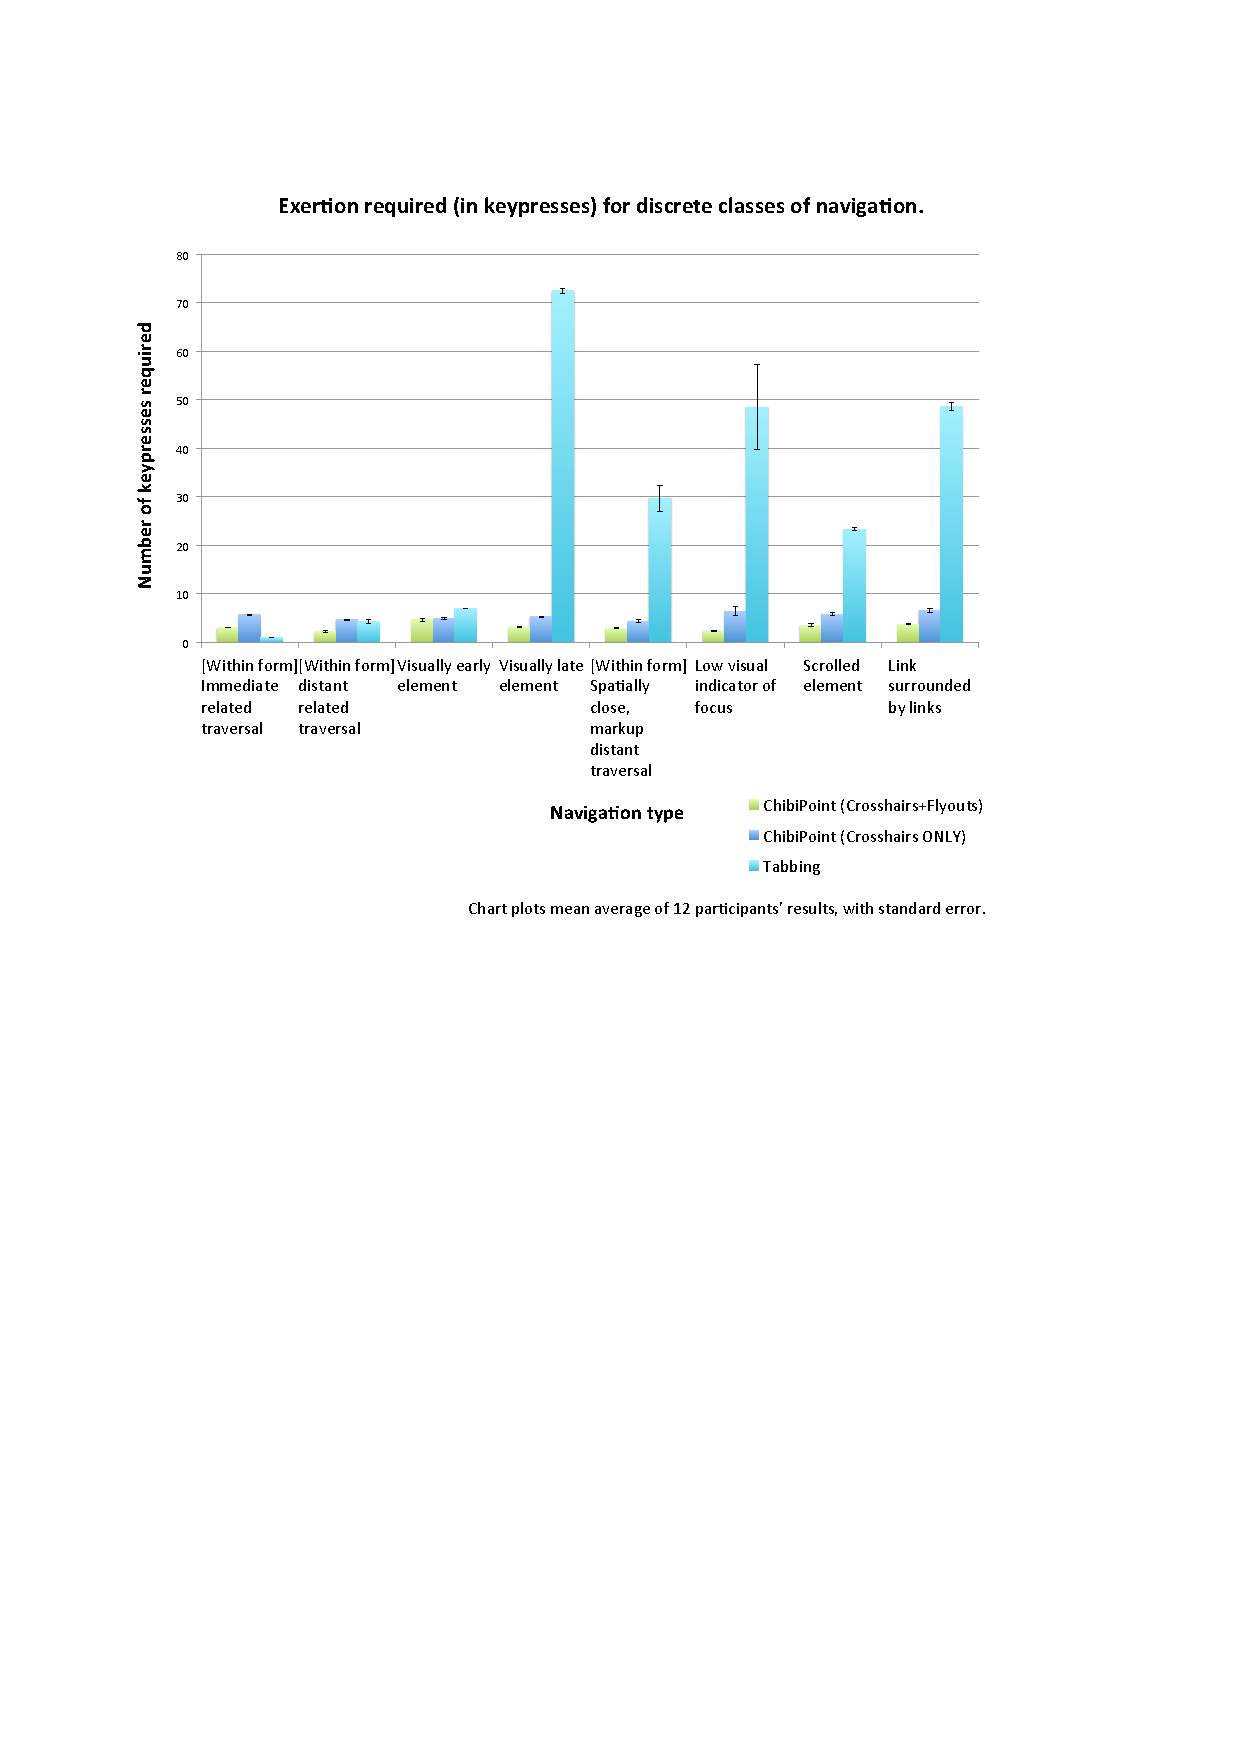
\includegraphics[width=8in]{figures/Exertion2.pdf}}
\caption{Exertion (in keypresses) per navigation task.}
\label{fig:exertion}
\end{figure}
\FloatBarrier
Visually it is evident that in the latter five tasks, the number of keypresses required for pointing by tabbing navigation is very large (>20). However, tabbing performance is lower (<10) for the first three tasks. Thus the performance across task types is inconsistent. Both ChibiPoint systems appear to have more stable behaviour --- never exceeding 10 keypresses. This is likely because hierarchical navigation can account for exponentially more targets with every lookup used, so it quickly becomes likely that a target can be pointed at.

More detailed statistical analysis ensues in the following sections. \Cref{sec:efficiencydiscussion} will appraise also the task differences in a qualitative sense, and explain the differences in performance.

\subsection{Efficiency Analysis by Task}
\newcounter{TaskType}
\newcommand{\navtask}[1]{\stepcounter{TaskType} \subsubsection{Task \arabic{TaskType}: #1}}
\navtask{[Within form] Immediate related traversal}
\begin{tabular}{l l}
\hline\hline %inserts double horizontal lines 
System & Keypresses Mean (s.d.) \\ [0.5ex] % inserts table 
%heading 
\hline % inserts single horizontal line 
CX & 5.67 (.492)\\
CX+F & 3.00 (.000)\\
Tabbing & 1.00 (.000)\\ [1ex] % [1ex] adds vertical space 
\hline %inserts single line 
\end{tabular}

Mean keystrokes differed statistically significantly between systems.\\
(F(1, 11) = 814.000, p < 0.001).

CX keystrokes significantly greater than Tabbing (p < 0.001).\\
Analysis failed to produce significance value for CX+F vs Tabbing.

CX+F keystrokes significantly fewer than CX (p < 0.001).

Hypothesis 1 refuted in this case.\\
Hypothesis 2 supported.

\navtask{[Within form] distant related traversal}
\begin{tabular}{l l}
\hline\hline %inserts double horizontal lines 
System & Keypresses Mean (s.d.) \\ [0.5ex] % inserts table 
%heading 
\hline % inserts single horizontal line 
CX & 4.67 (.492)\\
CX+F & 2.25 (.452)\\
Tabbing & 4.33 (1.155)\\ [1ex] % [1ex] adds vertical space 
\hline %inserts single line 
\end{tabular}

Mean keystrokes differed statistically significantly between systems.\\
(F(1.574, 17.311) = 33.543, p < 0.001).

CX keystrokes non-significantly different to Tabbing (p = 1.000).\\
CX+F keystrokes significantly fewer than Tabbing (p = .001).

CX+F keystrokes significantly fewer than CX (p < .001).

Hypothesis 1 supported (for CX+F only).\\
Hypothesis 2 supported.

\navtask{Visually early element}
\begin{tabular}{l l}
\hline\hline %inserts double horizontal lines 
System & Keypresses Mean (s.d.) \\ [0.5ex] % inserts table 
%heading 
\hline % inserts single horizontal line 
CX & 5.00 (.603)\\
CX+F & 4.67 (.888)\\
Tabbing & 7.00 (.000)\\ [1ex] % [1ex] adds vertical space 
\hline %inserts single line 
\end{tabular}

Mean keystrokes differed statistically significantly between systems.\\
(F(1.590, 17.489) = 54.057, p < 0.001).

CX keystrokes significantly fewer than Tabbing (p < .001).\\
CX+F keystrokes significantly fewer than Tabbing (p < .001).

CX+F keystrokes non-significantly different to CX (p = .797).

Hypothesis 1 supported.\\
Hypothesis 2 not supported.

\navtask{Visually late element}
\begin{tabular}{l l}
\hline\hline %inserts double horizontal lines 
System & Keypresses Mean (s.d.) \\ [0.5ex] % inserts table 
%heading 
\hline % inserts single horizontal line 
CX & 5.25 (.452)\\
CX+F & 3.17 (.577)\\
Tabbing & 72.50 (1.732)\\ [1ex] % [1ex] adds vertical space 
\hline %inserts single line 
\end{tabular}

Mean keystrokes differed statistically significantly between systems.\\
(F(1.246, 13.701) = 15056.088, p < 0.001).

CX keystrokes significantly fewer than Tabbing (p < .001).\\
CX+F keystrokes significantly fewer than Tabbing (p < .001).

CX+F keystrokes significantly fewer than CX (p < .001).

Hypothesis 1 supported.\\
Hypothesis 2 supported.

\navtask{[Within form] Spatially close, markup distant traversal}
\begin{tabular}{l l}
\hline\hline %inserts double horizontal lines 
System & Keypresses Mean (s.d.) \\ [0.5ex] % inserts table 
%heading 
\hline % inserts single horizontal line 
CX & 4.42 (.996)\\
CX+F & 2.92 (.289)\\
Tabbing & 29.75 (9.324)\\ [1ex] % [1ex] adds vertical space 
\hline %inserts single line 
\end{tabular}

Mean keystrokes differed statistically significantly between systems.\\
(F(1.017, 11.188) = 91.990, p < 0.001).

CX keystrokes significantly fewer than Tabbing (p < .001).\\
CX+F keystrokes significantly fewer than Tabbing (p < .001).

CX+F keystrokes significantly fewer than CX (p = .002).

Hypothesis 1 supported.\\
Hypothesis 2 supported.

\navtask{Low visual indicator of focus}
\begin{tabular}{l l}
\hline\hline %inserts double horizontal lines 
System & Keypresses Mean (s.d.) \\ [0.5ex] % inserts table 
%heading 
\hline % inserts single horizontal line 
CX & 6.42 (3.204)\\
CX+F & 2.33 (.492)\\
Tabbing & 48.50 (30.485)\\ [1ex] % [1ex] adds vertical space 
\hline %inserts single line 
\end{tabular}

Mean keystrokes differed statistically significantly between systems.\\
(F(1.012, 11.128) = 24.176, p < 0.001).

CX keystrokes significantly fewer than Tabbing (p = .002).\\
CX+F keystrokes significantly fewer than Tabbing (p = .001).

CX+F keystrokes significantly fewer than CX (p = .001).

Hypothesis 1 supported.\\
Hypothesis 2 supported.

\navtask{Scrolled element}
\begin{tabular}{l l}
\hline\hline %inserts double horizontal lines 
System & Keypresses Mean (s.d.) \\ [0.5ex] % inserts table 
%heading 
\hline % inserts single horizontal line 
CX & 5.83 (1.115)\\
CX+F & 3.50 (1.087)\\
Tabbing & 23.33 (11.155)\\ [1ex] % [1ex] adds vertical space 
\hline %inserts single line 
\end{tabular}

Mean keystrokes differed statistically significantly between systems.\\
(F(1.349, 14.837) = 1304.682, p < 0.001).

CX keystrokes significantly fewer than Tabbing (p < .001).\\
CX+F keystrokes significantly fewer than Tabbing (p < .001).

CX+F keystrokes significantly fewer than CX (p = .001).

Hypothesis 1 supported.\\
Hypothesis 2 supported.

\navtask{Link surrounded by links}
\begin{tabular}{l l}
\hline\hline %inserts double horizontal lines 
System & Keypresses Mean (s.d.) \\ [0.5ex] % inserts table 
%heading 
\hline % inserts single horizontal line 
CX & 6.67 (1.371)\\
CX+F & 3.75 (.452)\\
Tabbing & 48.67 (2.934)\\ [1ex] % [1ex] adds vertical space 
\hline %inserts single line 
\end{tabular}

Mean keystrokes differed statistically significantly between systems.\\
(F(1.387, 15.257) = 2296.627, p < 0.001).

CX keystrokes significantly fewer than Tabbing (p < .001).\\
CX+F keystrokes significantly fewer than Tabbing (p < .001).

CX+F keystrokes significantly fewer than CX (p < .001).

Hypothesis 1 supported.\\
Hypothesis 2 supported.

%
%
%
%
%

\subsection{Observational Analysis by Task}
\label{sec:efficiencydiscussion}
\setcounter{TaskType}{0}
\navtask{[Within form] Immediate related traversal}
This task demanded traversal in a login form from a `Username' field to its markup-adjacent `Password field'. Naturally this is a perfect task for tabbing, which achieves the navigation in just 1 keypress.

Both versions of ChibiPoint take at least that many keypresses just to invoke the interface.

In this particular case, pointing at the field's location took CX a relatively high number of lookups (>5). In some cases elements happen to line up in the center of one of the first constructed grids, allowing traversal in few lookups. Likewise there can also be positions on the page that take more lookups to navigate to, like this one. 

CX+F, once invoked, took only 2 keypresses (no variance), which is admirable efficiency considering ChibiPoint is not recruiting any data from the markup or current focus --- this is, for all intents and purposes, an arbitrary clickable in ChibiPoint's eyes.

\navtask{[Within form] distant related traversal}
This task, too, utilises tabbing's strength in form traversal --- however, it has to navigate this time to the end of a medium-sized form. This journey will be quite predictable (provided the form is marked up correctly), so the user knows in advance they have to press tab as many times as there are form elements to traverse.

Incidentally, some variance is seen in the tabbing results, despite the journey's being entirely deterministic. This is due to one participant's backpedaling through the form, possibly due to misunderstanding which target was the destination.

Unavoidably, tabbing demands more keypresses to traverse further in forms. Thus CX catches up in performance to tabbing in this task, with a non-significant difference in their means.

Meanwhile CX+F manages to overtake both systems significantly --- suggestions allow many form elements to be accessed, and CX+F can quickly drill through space enough to specify interest in the form.

\navtask{Visually early element}
Similarly to distant form traversal, tabbing is strong at traversing the first elements in a page's markup. There is some lack of predictability here, as it is non-guaranteed that the first element visually will be first also in the markup. Additionally there are invisible elements in the tab order: a `skip link' (see \Cref{sec:skiplinks}) to the page content, and a link to view an `accessibility help' document.

As early as the intended button is in the tab order, there are nonetheless enough elements in the way that the ChibiPoint systems' hierarchical trawls catch up with tabbing's linear trawl.

CX+F had the potential to out-perform CX here, but due to confusion in determining which flyout referred to which element, participants grew to either over-specify their target (until no other flyouts were offered), or otherwise fall back on the crosshairs mechanism for pointing. Thus in this case, the flyouts system did not significantly aid navigation.

It is worth disclosing also, that in this scenario, many mis-clicks were made due to CX+F's hard-to-distinguish suggestions. We discarded such attempts and had the participants attempt the task again until they succeeded. Thus this `first-time' performance is not strictly captured here.

Nevertheless, both ChibiPoint systems outperformed tabbing.

\navtask{Visually late element}
This test was particularly bad for tabbing, with >70 keypresses. If visual distance from the start of the page is to be taken as a heuristic for how much markup needs to be traversed to reach that element, then we should expect tabbing to require many lookups to reach the visually late element.

In particular, this was a page with many hyperlinks. There was a site-wide navigation bar at the top, as well as a navigation sidebar, each filled with hyperlinks to traverse. Even the page itself had many hyperlinks on it. Without a skipping mechanism, or starting the traversal from a position relatively close to the element in question, tabbing was at a disadvantage in this sort of task.

The performance of the ChibiPoint systems remained similar to the figures they had been producing until now; all elements are arbitrary to ChibiPoint, so it is immaterial how late the element is situated in the visual flow of the page.

CX+F out-performed CX here, since it was quickly able to convey interest in a specific area containing the hyperlink.

\navtask{[Within form] Spatially close, markup distant traversal}
This was a highly typical navigation case --- choosing the top search result after performing a search. This YouTube interface was task-oriented in its visual design, with the search results immediately adjacent to the search form. Here we test how well the heuristic of `visually close implies markup close' applies.

The markup of the page specified a longer journey than did its visual design. As such, tabbing exited the search form, and proceeded to traverse elements such as the login controls, then the site navigator, playlists and channel subscriptions. Only after this detour did it begin to navigate the search results.

Some variance was seen in tabbing, because with so many elements to be traversed, and an unpredictable journey, participants had little heuristic for how far they were from their target, and often overshot their destination in an attempt to hurry the navigation.

By comparison, both ChibiPoint systems performed significantly better, as they were not affected by this detour. CX+F's suggestions worked particularly well, as the search results were visually large, and thus featured in even broad spatial selections.

\navtask{Low visual indicator of focus}
This task showed well the potential ineffectiveness of tabbing. Amazon.co.uk was styled (intentionally or otherwise) to have no visual indicator of keyboard focus for a vast majority of its interacting elements. Though highlights existed, it was found that its controls listen for `mouseover' events rather than `focus', and thus give feedback only to the mouse.

Participants had to infer from the browser's `status bar' (a control which visualizes, amongst other things, the URL of any currently focused hyperlink), which element was focused. This information could come in forms such as: ``\begin{verbatim}http://www.amazon.co.uk/Polycotton-Hollowfibre-Non-Allergenic-Pillows-Pack/dp/B0029TA2LM/ref=sr_1_1?ie=UTF8&qid=1396716329&sr=8-1&keywords=pillow\end{verbatim}'', which was complex enough to be missed by many participants, who were observed to overshoot their target by pages, and even miss it on the way back also after backpedaling.

Far more effective were the ChibiPoint systems, which provided their own visual indicators over targeted elements. They were also more efficient, performing in far fewer lookups than tabbing.

\navtask{Scrolled element}
This task existed mainly to confirm that all systems were compatible with off-screen elements; once scrolled, this is simply equivalent to the `visually late element' test. It remains nevertheless an essential class of navigation to be compatible with, but the efficiency comparison is less important here.

Of particular note was that some participants realized in this task that they could recruit page scrolling as another vector to move elements under the ChibiPoint crosshairs, which re-assess targets on every viewport change.

\navtask{Link surrounded by links}
This task was designed to create problems for a suggestion-based system like `flyouts' --- it would explore whether users can cope with many suggestions packed densely into one place. This is more of a concern for time performance than it is for efficiency, as the number of keypresses is not affected (unless the user chooses to over-specify their target to reduce the number of suggestions to trawl through).

For tabbing this was not an interesting problem, although in a page populated densely with links, tabbing naturally has to traverse more controls.

We found that the number of keypresses required for flyout lookup was still a significant improvement on CX and on tabbing, so this situation apparently did not compromise CX+F's efficiency.

\section{Discussion}
\subsection{Support for Hypotheses}
% Hey, maybe ChibiPoint should be a less good citizen and always be listening for a numpad press? Or always be open?
The primary purpose of this evaluation was to ascertain whether our hypotheses, which pertain to system efficiency, were supported. We remind the reader again of those hypotheses (whose detail can be read in full at \Cref{chap:hypotheses}):

\textbf{\hypone}\\
\textbf{\hyptwo}\\

\subsection{Support for Hypothesis 1}
\newcounter{tasktablecounter}
\newcommand{\tasktablenumber}{\stepcounter{tasktablecounter}\arabic{tasktablecounter}.~}
\begin{tabular}{l l}
\hline\hline %inserts double horizontal lines 
Task & Supports / Refutes Hyp.1 \\ [0.5ex] % inserts table 
%heading 
\hline % inserts single horizontal line 
\tasktablenumber [Within form] Immediate related traversal & Refuted\\ \relax
\tasktablenumber [Within form] distant related traversal & Supported (for CX+F only)\\ \relax
\tasktablenumber Visually early element & Supported\\ \relax
\tasktablenumber Visually late element & Supported\\ \relax
\tasktablenumber [Within form] Spatially close, markup distant traversal & Supported\\ \relax
\tasktablenumber Low visual indicator of focus & Supported\\ \relax
\tasktablenumber Scrolled element & Supported\\ \relax
\tasktablenumber Link surrounded by links & Supported\\ [1ex] % [1ex] adds vertical space 
\hline %inserts single line 
\end{tabular}

Hypothesis 1 is supported for both versions of ChibiPoint in tasks 3--8 inclusive.\\
Hypothesis 1 is supported for CX+F, too, in task 2.\\
Hypothesis 1 is refuted in task 1 only.\\
Thus CX+F reduced keypresses compared to tabbing in 7 of 8 tasks, which we consider to be a large majority (>80\%).\\
CX reduced keypresses compared to tabbing in 6 of 8 tasks (75\%), which is certainly overall an improvement, but not the large majority sought by the hypothesis.\\
Since one mode of ChibiPoint (CX+F) meets the requirements, Hypothesis 1 holds.

\subsection{Support for Hypothesis 2}
\setcounter{tasktablecounter}{0}
\begin{tabular}{l l}
\hline\hline %inserts double horizontal lines 
Task & Supports / Refutes Hyp.2 \\ [0.5ex] % inserts table 
%heading 
\hline % inserts single horizontal line 
\tasktablenumber [Within form] Immediate related traversal & Supported\\ \relax
\tasktablenumber [Within form] distant related traversal & Supported\\ \relax
\tasktablenumber Visually early element & Not Supported\\ \relax
\tasktablenumber Visually late element & Supported\\ \relax
\tasktablenumber [Within form] Spatially close, markup distant traversal & Supported\\ \relax
\tasktablenumber Low visual indicator of focus & Supported\\ \relax
\tasktablenumber Scrolled element & Supported\\ \relax
\tasktablenumber Link surrounded by links & Supported\\ [1ex] % [1ex] adds vertical space 
\hline %inserts single line 
\end{tabular}

Hypothesis 2 is supported for tasks 1--2 inclusive, and 4--8 inclusive.\\
Hypothesis 2 is not refuted in task 3 --- it is merely not supported.
Thus CX+F reduced keypresses compared to CX in 7 of 8 tasks, which we consider to be a large majority (>80\%), as required.\\
It should also be observed that in the non-supported task, no refute was seen to the claim; in all cases, CX+F either outperforms or matches CX.

\subsection{How `effective' are the pointing systems under test?}
\subsubsection{Definition of effectiveness}
We promised in \Cref{sec:qualitative_promises} to deliver a more `effective' pointing system than tabbing. By this we mean: a system which is capable of completing the required pointing tasks. Tabbing was felt to be insufficient here, because its relative traversal was vulnerable to focus traps --- page regions beyond which focus cannot advance, or which indefinitely load new content into the path of traversal. Additionally tabbing was believed to be vulnerable to a `lack of visual indicator of focus' --- a situation where webpage elements provide no visual feedback upon keyboard focus, leaving the user lost.

\subsubsection{Tabbing effectiveness}
\label{sec:tabbing_effectiveness}
We did not attempt to capture the former effectiveness problem (focus traps), since we cannot do a quantitative comparison where one system is unable altogether to point at the target. However we capture some evidence for the latter effectiveness problem (lack of visual indicator of focus). This occurs, of course, in Task 6: Low Visual Indicator of Focus. A huge standard deviation in keystrokes (30.485) was measured on this task, especially considering the tabbing journey is deterministic, so no deviation need occur at all unless the user overshoots their target and has to backtrack.

Admittedly in many cases, participants overshoot on purpose, as they use (we believe) the visual progress of the tab focus as a heuristic for how many keypresses they need to input --- allowing them to pause less often to verify the element under focus. Hence a certain amount of deviation can be expected in longer navigations, as participants titrate their speed to traverse the long distances quickly.

Nevertheless, we feel the abnormally high deviation in the `low visual indicator of focus' task to be symptomatic of participants missing their target when using tabbing navigation --- they did not know that they were pointing at their target, and so continued traversing past it. This was confirmed by our observations of the task performance, and also from feedback the participants gave: \textit{``in some cases, e.g. Amazon, the button's were not highlighted so it required some careful investigation to find out what I was about to press''}, \textit{``when performing tabbing on the amazon page, I had very little knowledge about the current `location' of the tab. Even on websites that did show the location, it was often just a very faint dotted border, which really isn't much easier to see''}.

We assert at least that there exists an effectiveness problem with tabbing. However, ChibiPoint came with its own effectiveness problems.

\subsubsection{Flyout effectiveness}
\label{sec:flyout_effectiveness}
There existed some praise for the flyouts system, with one participant saying \textit{``Chibi with flyovers [sic] worked great!''} --- possibly this can be interpreted as an assessment that it solved the tasks well, which would imply effectiveness. In the same vein, ChibiPoint with flyouts was described to \textit{``work just as well and often better in all cases [than tabbing]''}.

Flyouts were found, however, to obscure the elements that participants tried to point at: \textit{``Sometimes when using flyouts on an area with many links, the suggestions would become a bit cluttered making it slightly difficult to see what I was pointing at''}. The same participant, however, was unperturbed by this: \textit{``However, by choosing flyouts, this is a sacrifice I am willing to make (and understand why)''}, suggesting that this is still an acceptable level of effectiveness. It must also be pointed out that tasks such as `Link surrounded by many links' were designed to be worst-case scenarios for the flyouts system.

Using colour-matching to designate which flyout referred to which clickable was felt to be at least partially ineffective: \textit{``question the effectiveness of the use of colours to highlight the link suggestions. On a webpage with a lot of colours this just because [sic] confusing''}. The positioning of the flyouts was felt to be confusing also \textit{``especially when the key shortcuts [...] overlapped and the shortcut appeared over the face of other links''}. This is a hard problem to solve, but we suggest nevertheless some alternative designs:

\begin{itemize}
\item Positioning the flyout on the clickable it describes could make it easier to determine which element it refers to, but at the same time it necessarily obscures that clickable. However the user might not need to see the entirety of a clickable to be able to act on it, so this could be fine, and work better than the current confusion.
\item Reducing the number of flyouts could sacrifice efficiency to improve effectiveness; less colours will be in use, and less flyouts exist to overlap each other or each others' clickables.
\item Change the avoidance algorithm (see \Cref{sec:avoidance}) so that flyouts further avoid overlapping each other, and perhaps design it also to avoid overlapping each others' clickables.
\item Make flyouts partially transparent, to limit the occlusion they can cause.
\end{itemize}

It has to be cautioned also that we have not captured expert performance in this study --- the current design could be acceptable to an experienced user.

\subsubsection{Crosshair effectiveness}
Crosshairs did not utilise the same `clickable' detection that flyouts enjoyed. We chose this implementation because there was an advantage to this: clicks could be sent to elements which were not recognised as clickable by our system.

However this posed an effectiveness problem: participants were unsure whether the targeted element was one that a click could be sent to. Especially when containers existed around clickables, participants sometimes clicked these in stead of the clickable itself, assuming that it listened for click events.

Feedback reveals such experiences: \textit{``Chibi with just crosshairs was unique and I found it efficient, though having the html container light up was confusing''}.

Possibly a compromise design exists: allow users to click elements with crosshairs regardless of whether a clickable is detected, but `paint' that target a specific colour whenever it is known for certain to be clickable. This solution gives the user power to click whatever they want, but also feedback of what might happen if they do.

Overall (it is unclear if flyouts are included in this assessment), ChibiPoint was felt to be \textit{``far less variable than tabbing.''}. That is, its performance was consistent over a variety of tasks. This in itself can be taken as a type of effectiveness --- it is suited to more pointing contexts.

\subsection{How `predictable' are the pointing systems under test?}
\subsubsection{Definition of predictability}
We promised in \Cref{sec:qualitative_promises} to deliver a more `predictable' pointing system than tabbing. By this we mean: a pointing system where the user knows in advance what the outcomes of their actions will be (ie, what output will arise from each of their inputs). We felt tabbing to be fundamentally `unpredictable' because it traverses with respect to the page markup --- its journey is based on code the user cannot see. 

\subsubsection{Tabbing predictability}
We capture quantitatively some evidence for a predictability problem in tabbing. Since the system is meant to take a deterministic route through the page (the markup does not change, and the route cannot branch, except with skiplinks which we did not use), one might expect there to be no deviation in the scores of participants. But as discussed in \Cref{sec:tabbing_effectiveness}, one reason for deviation in keystroke scores of participants, is that users overshoot their target in their haste to pre-empt how many keypresses are required. This is because a visual heuristic is used to judge progress in a (non-visual) markup traversal.

\subsubsection{Flyouts predictability}
% usability study covers some stuff, right?
One participant suggested implementing \textit{``a priority system in the background that chooses which keys to highlight based on previous browsing history rather than what seems like random''}, implying that the suggestions produced by flyouts could not be pre-empted. This is not a huge failing: the flyout feature on its own is not intended to enhance predictability; its primary goal is adding efficiency.

In any case, participants were observed to exercise some control over their shortlist of flyouts, as evidenced by their over-specifying of elements on tasks like `visually early element', to remove confusing suggestions. So users understood how to constrain their search, bounding the possible suggestions, even if they did not know which possibilities would be presented.

\subsubsection{Crosshairs predictability}
ChibiPoint overall was described by one participant as \textit{``very intuitive and was simple to use. Also, it mapped well to the Numpad which made navigation easier and more `familiar' so to speak''}. We take this `intuitivity' to meet our definition of predictability --- a user's knowing in advance what the outcomes of their actions will be. Mappings to numpad directions were understood, so it is possible that this participant understood that they had non-arbitrary control over the direction of traversal.

Incidentally, several participants warned that losing this spatial mapping of inputs would harm the system --- \textit{``Numpad is very handy for the grid interface and touch typing. It would be tricky to use the number row on a laptop keyboard, though''}. For laptop keyboards we have developed another $3\times3$ grid mapping of keybindings, that does not require a numpad (and uses instead a grid of alphabet keys). This has been received well (outside of a formal study context) by users who lacked a numpad.

\subsection{User Preferences}
User preferences are tabulated in \Cref{fig:quantpost}. 10 participants (83\%) chose CX+F as their preferred system. The only deviations from these were 2 participants who chose CX. No participant preferred Tabbing. That any users explicitly preferred to not have flyouts is symptomatic that there are matters other than efficiency involved in system preference. This might be accounted for by the effectiveness problems we discussed in \Cref{sec:flyout_effectiveness}. Overall though, it is heartening to see that both ChibiPoint systems are preferred to Tabbing.

Asked to rate ease of use on a 5-point scale (with 1 being the lowest), ChibiPoint systems averaged highly (CX = 4.17/5, CX+F = 4.75/5), and certainly higher than tabbing (2.08/5).

Despite effectiveness issues raised by flyouts, users felt it made ChibiPoint easier to use. Of course, this is a subjective question and `ease of use' may have been felt to include the number of keypresses required --- users could just be referring to efficiency here.

The amount of keypressing required by ChibiPoint was considered reasonable (`unreasonability' rating CX = 2.08/5, CX+F = 1.42/5), and tabbing considered completely unreasonable (4.75/5).

Thus it was seen that users agree with the hypotheses we have supported quantitatively --- that ChibiPoint systems are more efficient than tabbing, and also that flyouts improve that efficiency further.

\section{Summary}


\chapter{Conclusions \& Future work}
\label{chap:conclusions}
[Revisit this once Results section is finalized]

\pagebreak
\chapter{Glossary}
\printglossary

%\nocite{*}
%\nocite{Doe:2009:Online}
\clearpage

%\renewcommand*{\theHchapter}{\Alph{chapter}}
%\stepcounter{chapter}

\phantomsection
\addcontentsline{toc}{chapter}{References}
\printbibliography

\clearpage
\phantomsection
%\pagebreak
\addcontentsline{toc}{chapter}{APPENDICES}
\appendix
\chapter{Pilot Study}

\begin{figure}[ht]
% table row height
\renewcommand{\arraystretch}{1.5}

\begin{tabularx}{\textwidth}{X|X}
\hline\hline %inserts double horizontal lines 
Question & Response \\ [0.5ex] % inserts table 
\hline
%heading 
Gender	&	Male	\\
Age	&	23	\\
How many hours a day do you use a computer or smartphone?	&	13+	\\
How proficient are you at controlling computers with just the keyboard?	&	I use hotkeys in addition to a mouse/pointing device	\\
Do you /currently/ have any motor impairments/disabilities that hinder computer usage? If so, please explain.	&	None	\\
Do you presently have any difficulty reading the screen? If so, please explain.	&	None	\\
Have you ever had any motor impairments/disabilities that hinder computer usage? If so, please explain.	&	None	\\
What is the main desktop OS you use?	&	Windows	\\
What is the main web browser you use?	&	Internet Explorer	\\
Have you ever used any accessibility software or hardware to control computers? If so, please explain which, and the extent to which you used them.	&	Developed and used adaptive interface software for World of Warcraft.	\\
Is there any additional information you wish to declare?	&	None	\\
How proficient are you at touch-typing?	&	5	\\
What is your occupation?	&	Software research engineer	\\ [1ex] % [1ex] adds vertical space 
\hline %inserts single line 
\end{tabularx}
\caption{Questionnaire response of Pilot Study participant}
\label{fig:partic_pilotpre}
\end{figure}

\begin{figure}[ht]
% table row height
\renewcommand{\arraystretch}{1.5}

\begin{tabularx}{\textwidth}{X|X}
\hline\hline %inserts double horizontal lines 
Question & Response \\ [0.5ex] % inserts table
\hline 
Which system did you prefer using?	&	ChibiPoint (with crosshairs AND flyouts)	\\
How easy was it to point using `tabbing navigation'?	&	1	\\
How was the amount of keypressing required in `tabbing navigation'?	&	5	\\
How easy was it to point using `ChibiPoint (with just crosshairs)'?	&	4	\\
How was the amount of keypressing required in `ChibiPoint (with just crosshairs)'?	&	2	\\
How easy was it to point using `ChibiPoint (with crosshairs AND flyouts)'?	&	5	\\
How was the amount of keypressing required in `ChibiPoint (with crosshairs AND flyouts)'?	&	1	\\
Have you any other feedback?	&	Crosshairs without flyouts can be difficult to accurately pinpoint the desired text.	\\
\hline %inserts single line 
\end{tabularx}
\caption{Post-experiment questionnaire response of Pilot Study participant}
Ratings were all on a five-point scale, 1--5.
\label{fig:partic_pilotpost}
\end{figure}

\chapter{Usability Study}

\definecolor{mygreen}{rgb}{0,0.6,0}
\definecolor{mygray}{rgb}{0.5,0.5,0.5}
\definecolor{mymauve}{rgb}{0.58,0,0.82}

\lstdefinelanguage{custom}
{
morekeywords={R},
ndkeywords={P},
sensitive=false,
morecomment=[l]{//},
morecomment=[s]{/*}{*/},
morestring=[b]{*},
moreemph=[4][b]{=},
literate={ö}{{\"o}}1
           {Ü}{{\"U}}1
           {ü}{{\"u}}1
}

\lstdefinestyle{basic}{ %
  backgroundcolor=\color{white},   % choose the background color; you must add \usepackage{color} or \usepackage{xcolor}
  basicstyle=\footnotesize\ttfamily,        % the size of the fonts that are used for the code
  %\ttfamily
  %\sffamily
  emphstyle=\color{red},
  breakatwhitespace=false,         % sets if automatic breaks should only happen at whitespace
  breaklines=true,                 % sets automatic line breaking
  captionpos=t,                    % sets the caption-position to bottom
  commentstyle=\color{mygreen},    % comment style
  deletekeywords={...},            % if you want to delete keywords from the given language
  escapeinside={\%*}{*)},          % if you want to add LaTeX within your code
  extendedchars=true,              % lets you use non-ASCII characters; for 8-bits encodings only, does not work with UTF-8
  frame=single,                    % adds a frame around the code
  keepspaces=true,                 % keeps spaces in text, useful for keeping indentation of code (possibly needs columns=flexible)
  keywordstyle=\color{blue}\bfseries,       % keyword style
  ndkeywordstyle=\color{red}, % another keyword style
  %language=Octave,                 % the language of the code
  morekeywords={*,...},            % if you want to add more keywords to the set
  numbers=left,                    % where to put the line-numbers; possible values are (none, left, right)
  numbersep=20pt,                   % how far the line-numbers are from the code
  numberstyle=\tiny\color{mygray}, % the style that is used for the line-numbers
  rulecolor=\color{black},         % if not set, the frame-color may be changed on line-breaks within not-black text (e.g. comments (green here))
  showspaces=false,                % show spaces everywhere adding particular underscores; it overrides 'showstringspaces'
  showstringspaces=false,          % underline spaces within strings only
  showtabs=false,                  % show tabs within strings adding particular underscores
  stepnumber=1,                    % the step between two line-numbers. If it's 1, each line will be numbered
  stringstyle=\color{violet},     % string literal style
  tabsize=4,                       % sets default tabsize to 2 spaces
  %title=\lstname                   % show the filename of files included with \lstinputlisting; also try caption instead of title
  %inputencoding=utf8/latin1
}

\begin{lstlisting}[caption={Transcript of Usability Study}, label={lst:usabilityTrans}, style=basic, language=custom, flexiblecolumns=true]
R: (Researcher)
P: (Participant)

====Flyouts On====

	First system, Flyouts ON.

R:	Start the system by pressing Apple K.
P:		Okay, is there an Apple on here?
R:	Yeah, I've mapped Ctrl to Apple.
P:		Okay, great.
P:		I'll do what I have to do to get started, and...
		*Presses Apple K*
		*Chibipoint interface appears*
P:		Okay.

R:	Your mission, should you choose to accept it, is to search for the Olympics.
P:		Oh, search, okay, so...
		*Presses indicated key to drill toward top-right quadrant, where search is*
		// No instruction required on how to point, or what keys to use!
P:		And now, the question is... oh, I see.
		*Continues drilling toward search box*

P:		Uh, it keeps coming...
		*Continues drilling toward search box.*
	[Field is now in crosshairs.]
P:		Ah!
P:		Am I there yet?
		*Guesses key*
P:		Nope. Do I have to hit return or something?
		*Hits return*
		*Search field is selected*
		// No instructions required!
		*Types Olympics, submits search*

P:		Who would search for the olympics... haha! Okay, now what?
P:		I might have to do the same again. Ctrl K?
		*Presses Apple K*
		*Chibipoint interface appears*
P:		Okay, what have I got to do?

R:	Let me think, what would be a good idea.. try and hit that article, Sochi 2014 [top result].
P:		Hm, oh the first Sochi 2012? Sochi 2014, dude! Haha.
P:		The one with that guy, the one with the picture.
		*Drills toward article*
		*Drills toward article*
P:		And it's missed the link..
P:		Oh, I see.
		*Activates an appropriate flyout*
		// Unprompted! Only one lookup later than expert perf.
P:		It does that. Very clever of you, that extra thing.

P:		Hm, okay. This is great! I would totally take this.
		*Presses Apple K*
		*Chibipoint interface appears*
P:		Especially as it's keyboard, and it saves you from moving to it.
P:		And it's not slower than, uh, mouse; you don't have to move it to. So that's great.
P:		I used to keep the mouse on this; it's obnoxiously slow. I used to use that in 1998, when I was working for Lego, I was so screwed up I did use that sometimes.
P:		Anyway, yes.

R:	Now click on Sport.
R:	Err, that sport.
P:		Oh, that sport up there.
		*Drills toward*
P:		Mm, (counting noises)
		*Presses wrong flyout*
P:		Oops, missed. So what's the back button?
R:	Backspace.
		*Presses back*

P:		Let's try again.
		*Presses Apple K*
		*Chibipoint interface appears*
P:		Okay.
		*Drills toward*
P:		Mm.
		*Again activates inappropriate flyout*
P:		Ah, it's, it's.. there's something wrong.
P:		I hate to tell you this, but I'm definitely clicking on the right thing. Haha.

R:	Okay, uh..
P:		I guess I could therefore try to compensate for that one, cause..
		*Drills toward*
R:	I dunno how much I should say..
		*Activates correct flyout*
P:		Yeah, okay. I compensated, but there's definitely something wrong. Haha.

R:	Okay, how about a different website; go to Amazon.
		*Changes website*
		*Presses Apple K*
		*Chibipoint interface appears*
R:	Let's do a... I dunno; let's do a search.
P:		Okay.
		*Drills toward*
		*Many flyouts appear close together with tags tying them to their buttons in various directions*
P:		Hah! That's really all over.
		*Presses appropriate flyout for search field*
R:	Hm, what's your favourite book?
		[search term redacted]
		[discussion of how to select suggested products using arrow keys on accessible input device]
		*search submitted*

R:	Try and click on [author for first result redacted].
		*Some unproductive inputs [accessible input device typing in wrong mode]*
P:		Hello?
P:		Oh, I've got to...
		*Presses Apple K*
		*Chibipoint interface appears*
		*Drills toward*
		*Presses appropriate flyout*
		//  Expert performance already!

R:	I wonder if that's enough for Amazon. Let's go to Wikipedia.
R:	Looks like it's already selected the input field. Shall we pretend it didn't?
P:		Why? Why don't you just have me go to the German [Wikipedia] or something?
		*Presses Apple K*
		*Chibipoint interface appears*
P:		Let's go to the German one.
R:	Okay.
		*Presses appropriate flyout*
		// No drilling required!

P:		Okay, now what?
		*Presses Apple K*
		*Chibipoint interface appears*
		*Drills toward search*
		*Drills toward search*
		*Drills toward search*
R:	German foods?
		*Presses appropriate flyout*
		*Searches currywurst*

R:	Let's go to the bottom; there should be some interesting markup there.
		*Scrolls to end*
R:	Alright, let's go to Über Wikipedia.
P:		Alright.
		*Drills toward*
		*Presses appropriate flyout*

	[Discussion to find an inaccessible website to navigate next]

		*Google searches Bath Chronicle.*
		*Presses Apple K*
		*Chibipoint interface appears*
		*Presses key for appropriate flyout*
		*Bug in Chibipoint means the key press is caught by Google instead*
P:		That's interesting. So the `J' got captured.
		*More typing*
P:		Yeah, every time you type something, Google's capturing it.
P:		Yeah, so, can't... it's just totally failing now.

R:	Yeah, there's still other ways to use Google with the keyboard.
R:	I found this earlier. I don't know how to make my key listeners the highest priority.
R:	It's JavaScript injected into the page, so it's fighting the rest of the page.
P:		So we can cheat briefly.
		*Clicks news article of Bath Chronicle*

P:		So now..
		*Presses Apple K*
		*Chibipoint interface appears*
P:		So what do you want me to click?
		*Drills toward top-left*
R:	Click `place an advert'.
		*Presses appropriate flyout*

R:	Register. Let's see how it does with forms.
P:		Okay.
		*Presses Apple K*
		*Chibipoint interface appears*
		*Drills toward Register*
		*Closes Chibipoint accidentally*
P:		Oops.
		*Presses Apple K*
		*Chibipoint interface appears*
		*(Immediately) drills to original position*
		// Appears to be able to reproduce practiced spatial traversals quickly without pausing to think.
P:		...That's a 'Z'; okay. [Text was obscured, so appeared as numeral 7]
		*Drills toward*
		*Drills toward*
	[No flyouts have appeared for this button; clickable detection failed, so crosshairs are the only option. It's now in crosshairs.]
		*Presses enter*

	[A form appears]
		*Tabs a few times to enter form*
		// Candidate seems to notice that both systems can co-exist. This tab journey was a short one.
P:		Oops.
		*Presses Apple K*
		*Chibipoint interface appears*
	[First 6 fields of form have flyouts suggested, without drilling.]
		*Presses flyout for first form element*
		*Focuses drop-down menu*
P:		Heh. Yeah, thanks. [Presumably wanted menu to open, as with a real click].
		*Starts filling out form (unprompted) without Chibipoint*
		*Accidentally closes window.*

		*Restores window.*
		*Presses Apple K*
		*Chibipoint interface appears*
		*Drills toward `Address lookup' button*
		*Drills toward [non-trivial because it's on an edge after each drill, and also because no flyouts are offered; clickables detection failed]*
		*Drills toward [now in crosshairs]*
		*Presses Return*
		*Address lookup is clicked; panel appears overlaying existing content*

		*A focusing keypress is made, possibly tab or Apple L (select address bar). It is not clear if this is intentional.*
		*Keyboard focus leaves browser*
		*Presses Apple K*
		*Chibipoint interface appears*
		*Attempts to drill, but keyboard focus is in the address bar; types into address instead.*
	[Much attempting to regain focus and resume drilling, but even tabbing fails]
	[Resort to mouse click to put focus back in browser content pane]

		*Drills toward address*
		*Drills toward*
		*Drills toward address [now in crosshairs, though never detected by flyouts]*
		*Presses return*
		*Click sent, element flashes, but no change in form*
		// Without mouseover probing, we cannot get affordances for which element needs to be clicked, and confused results can occur.
	[Attempt to verify using mouse which element is meant to be clicked]
	[Panel closes]

	[Recover panel by refreshing page and re-opening Address lookup]
	[Clicks same element again with Chibipoint; form option remains unclicked]
P:		It must want [me to click] the checkbox next to it.
		*Presses Apple K*
		*Chibipoint interface appears*
		*Drills toward*
		*Drills toward*
		*Drills toward*
	[Button is not yet in crosshairs. Drilling labels now hidden since grid is small.]
P:		Hmh.
		*Presses return*
P:		Yeah, I have no idea. It doesn't seem to be..
P:		So, does that..
		*Hovers mouse over to confirm feedback*
P:		[The button] doesn't seem to notice [with Chibipoint] that something's there.
P:		Obviously there's no signal that [an emulated mouse cursor is above].
P:		`Cause the [cursor] changes into a hand when you hover over it.
	[Repeats previous navigation:]
		*Presses Apple K*
		*Chibipoint interface appears*
		*Drills toward*
		*Drills toward*
		*Drills toward*
	[Button is not yet in crosshairs. Drilling labels now hidden since grid is small.]
		*Presses return*
		// Seems to think that when the drilling labels are gone, it is not possible to continue drilling.

		*Reopens Chibipoint, drills lightly into an alternative journey.*
		*Closes Chibipoint without clicking*

		*Reopens Chibipoint, redoing a previous journey.*
P:		Yeah, nothing I do seems to get the tick.
R:	Try pressing [bottom-left quadrant (now unlabelled)]
		*Drills*
R:	And again.
		*Drills*
R:	You can inch closer.

R:	Boxes aren't perfect sub-boxes; they grow a little bit.
P:		Okay. I didn't see Z as an action, so...
R:	Ah. Yes, it... I can't make text any smaller.
P:		Well, is that enough information?





	====Flyouts Off====

R:	Now try a version with the Flyouts turned off.
P:		Okay.
	[On BBC homepage]
		*Presses Apple K*
		*Chibipoint interface appears*
R:	Try and watch Top Gear. [This is at the very bottom edge of the grid]
P:		Okay, down there.	
		*Drills toward*
		*Drills toward*
		*Drills toward*
		*Presses return*
	[Page navigates]
		// Even buttons in tricky positions were able to be clicked easily.

		*Presses Apple K*
		*Chibipoint interface appears*
	[Top Gear Flash pane is painted wholly by Chibipoint; inner structure not detected]
		*Presses space bar to attempt to play video*
	[Page scrolls upon space bar since video does not have focus]
		*Drills toward Flash pane*
		*Drills toward centre of Flash pane*
		*Presses return*
	[Flash pane is clicked, but no meaningful change occurs]
		*Presses key to scroll up*
	[Page does not scroll, despite input]
P:		How do you scroll up?
R:	Your focus is trapped by Flash.
	[Mouse recruited to recover focus]
	[Page scrolled back to beginning]

		*Presses Apple K*
		*Chibipoint interface appears*
P:		So, is the big yellow thing..? I'm sure if it could just see which button I'm trying to click..
P:		No, it's not doing anything.
		*Presses Apple K*
		*Chibipoint interface appears*
		*Closes Chibipoint*

R:	So I'll spoil that; Flash players can't take clicks [from ChibiPoint].
P:		Oh, okay.
R:	So you've discovered that.

	[We return to BBC homepage]
R:	Try to click something on the bottom of the page - that's not on-screen.
R:	Music.
		*Presses Apple K*
		*Chibipoint interface appears*
		*Scrolls using Page Down*
		// Unprompted, understands that page scrolling keys co-exist with ChibiPoint.
		*Drills toward an element in the same list as `Music'*
P:		Too late; I'm going to go into `Learning'.
P:		Although it's actually not what you said.
	[Actual `Learning' text is not highlighted, but clicking the box that contains it worked in this case; did not have to drill too specifically]
		*Presses return*
	[Navigates to Learning]

R:	Let's see if there's anything hard to click on; keep scrolling.
		*Presses Page Down*
R:	Click the `Accessibility Help'.
P:		Okay.
		*Presses Apple K*
		*Chibipoint interface appears*
		*Drills toward*
P:		Hmm..
		*Drills toward*
	[Painting of link container obscures the white hyperlinks within]
R:	Oh god.
		*Drills toward*
	[Presently highlighted element is the link below Accessibility Help]
P:		And then, how do you move it around? Did you say the Z key..
R:	The keybindings continue to be exactly the same.
P:		Oh, but I didn't memorise them.
R:	Uhh.. they're this grid.
	[Demonstrates grid of 9 keys on accessibility hardware that map to on-screen controls]
P:		Oh, okay, so..
		*Drills toward*
		*Presses enter*
	[Accessibility Help is clicked]

R:	So, did you notice that they were...
P:		No, I totally didn't notice that they were,
P:		and I shouldn't, since there was a cue.
		// Mapping was not noticed nor memorised; singular lack of incidental information.
P:		Okay.
P:		
P:		Okay, so..
	[Decides to click one of the webpage accessibility articles]
		*Presses Apple K*
		*Chibipoint interface appears*
		*Drills toward*
		*Drills toward*
		*Drills toward*
		*Presses return*

P:		Well anyway, this doesn't seem to be a problem, so..
R:	Right, I'll end.





	====Feedback====

R:	What do you think of the two systems you tried (flyouts on, off)?
P:		I couldn't tell the difference, I'm afraid.
P:		What was the... oh, I dunno... oh, the flyouts with commas and periods and things?
R:	Yeah.
P:		Yeah, I liked the commas and periods and things. They were pretty good guesses. Although it was a bit cluttered. I'd like to be able to switch back and forth depending on what I was trying to do.
R:	Uhh, by switch back and forth, do you mean `hide them'?
P:		Yeah. Exactly, so like mostly it's great. Although anyway you can hide it with Ctrl-K, so I guess that's enough.

R:	Was the problem that [the flyouts] obscured [what you were trying to point at]?
P:		It just looks a bit cluttered sometimes. But it was really useful, so I think I'd probably mostly just have them on. I could just imagine, I dunno some time I might want to turn them off...

R:	Would it be useful to have, like, holding down SHIFT dispels the interface?
P:		What?
R:	Uhm, there's a lot of heads-up display on the page; you could hold down a modifying key to hide stuff temporarily, but not lose where your grid is.
P:		Uhh, I don't know what... one thing is that Ctrl-K doesn't work very well for me, `cause I use emacs; that's why it was after a little while when I was doing the wrong things because I doing the wrong commands, because I was confusing all the commands.
P:		So for me it would be better if it was something different, like Alt+something, just because I hardly ever use Alt. Then I'd remember it; I could remember that. And also, when I'm on emacs, I'd be able to control it.

R:	There's a limit to what keyboard shortcuts I'm allowed to choose. Actually, it's a limit to what I can `suggest' as a keyboard shortcut, but the user can override the system ones if they manually choose them.
P:		Okay. Yeah.
R:	So that could be done.

P:		Yeah, but it was really nice. It was a nice way to do it.
P:		I could imagine using that a lot.
P:		Although now I'm pretty much just using the pen tablet.
P:		But it saves you find the tablet - the pen, tablet; it's just right there.

R:	Were there any things that you didn't understand?
P:		Oh yeah, like I said, I didn't notice that the grid was continuing; or rather I didn't pick up that - they just looked like random letters to me. I didn't know why you were doing it.
P:		But had I noticed... `cause, the thing is that in the old days, my first guess would've been, was the right hand.
P:		In the old days, the arrow keys used to be right around there.
P:		I should've picked up that you were using the left hand instead, but I didn't.
R:	I'm less worried about that, because it usually would be the numpad, but it's [accessible input device] mode.
P:		Yeah, okay. The problem would be the - because they were slowing down the typist, when you're in Qwerty, all the characters that you use are mostly on the left, so you wouldn't normally expect them to use the right hand for the arrow keys.
R:	Okay, so they can be swapped.

R:	Did you ever desire to be able to `undo' a drill-down, and retreat?
P:		Yeah, once, and what I did was just Ctrl+K to start over, but there was, like, one time.
R:	Okay. There's a feature I should've disclosed to you; there is a key that can `back up'.
P:		Okay. Yeah, no, I would've wanted that if I was, I got it.
P:		But that was pretty fast; considering how long it took me to get... quite a lot of usability stuff downloads, the first time you try using a pen tablet(!), yeah, so that was, I was able to get into that; that was fine.
P:		Again, I am old, and I did used to navigate with the arrow keys on the other hand(!)

R:	Would you say it's intuitive?
P:		It was largely intuitive; I mean, there was a couple things you didn't know. It might be nice to have, like, a little helping thing that could pop up and tell you the cheat sheet, to tell you if there's any other stuff.
P:		`Cause usually what I do is, I hack around a bit with the command, and then I go and read the manual, and see if there's anything I've missed.
P:		So this was a very successful first hack-around, but then you would want somewhere to be able to read and find out what you'd missed.
R:	Maybe I'll print a cheat-sheet rather than coding one.
P:		Yeah, sure.

R:	Were the `clickable' suggestions - made by the flyouts - were they good enough guesses?
P:		Yeah! Yeah, they were highly accurate; I was very impressed by that.
P:		I especially liked that they were sometimes, you picked the wrong region, and they still guessed that it was just slightly off the region; it was like, way! Thinking outside the box.

R:	Did you find that there were any things that it didn't seem to be able to see?
P:		I didn't notice any in particular - except for something, you know, that one thing that we tried over and over again, and couldn't get anything to see.
R:	That button didn't seem to be marked up properly.
P:		Yeah.
R:	It has a lot of intelligence to work out if something's clickable, but...
P:		But somehow, like I said with the mouse you could hover over it and it would change into a pointy thing, so there must be something there, but it wasn't much.
R:	I put in a feature to force it to `mouseover' anything that the crosshairs are on. But it doesn't seem to... I told it to trigger the mouseovers, but it never happens.
P:		I never really `got' the crosshairs, so I hadn't realised - right until the end you showed it to me - but I didn't earlier pick up on that.

R:	Yeah, it's problematic that as well as the flyouts, there's also the crosshairs.
P:		Okay. I wasn't really noticing [the crosshairs], because the other system was working so well for me, so I was sort of reflecting, and concentrating on what I saw.
R:	And yet, once you were switched to the system without flyouts, you were happy to use crosshairs.
P:		Well, once you showed me how to use them, that you could still navigate even if there's no letters, and then I was like, okay, well that was like what I was used to before with the [accessible input device], so I learned my lesson.

R:	Would you say you could understand how to get to a place?
P:		Yeah, obviously; you just saw me do it(!)
R:	Was the grid-splitting an intuitive way?
P:		Yeah, no, I thought that was fine; that was great. Uh, yeah, that made sense. I liked that it was very bright, and there was this little {unclear}.
P:		I'm probably not your best - it depends how you think about it. I'm probably not the most stereotypical - it's not like taking home a heavier[?] - somebody who doesn't use a computer - to try it.
R:	Well, it's designed for [people with accessibility requirements]. You'd probably be a pretty good sample for accessibility needs.
P:		Well, if it's designed for disabled people with a lot of experience with different tech, so that's what I'm saying - you'd need to find some other people who haven't had the same breadth of experience of available tech.

R:	If we want to model performance of an expert, that's fine though.
P:		Yeah, no, that's fine. I'm just saying that you should realise I'm not a typical user. In fact, that's one of the things that Google will tell you, probably(!) is that their problem is that all the people they hire are not at all - can't even conceive of the problems that their users have. Figuring out, for example, that keyboards {unclear}(!)
P:		Uhm, yeah, we're not the normal. I'm particularly mechanically inclined, so I tend to figure these things out pretty quickly.
P:		But still, it was good. I'm just saying that the hacking through it might not... well of course, to be fair, who does hack through your stuff? People who are good at hacking. Look at the manual.

R:	How do you feel this system compares to navigating using tabbing around a page?
P:		Oh, it's obviously faster because it's hierarchical. My first-years should be able to answer that question.
R:	Would you prefer this system?
P:		To tabbing? Of course, yeah. As long as it didn't interfere with anything else.

R:	Bonus question: how does it compare to the mouse?
P:		Uh, like I said, the main benefit is... well, there's actually two benefits. The main benefit is that for me, because of whatever - I don't know if everybody has this - is that especially by the time you get your hand over, and you find the mouse, that sort of thing, it was just much faster to have it right on the keyboard.
P:		So, that's... and the other thing is that, honestly, sometimes it's really hard to click on, so being able to choose a letter is just better than, than just, life, you know, even with a pointing device.
P:		But, yeah. So, basically, dunno, I'd have to try it. Uh, it might be... the other, the downside is that one of the problems with typing injuries is that you are too much in the same posture doing the same thing all the time, so it is good to use other devices if you have them, just to move around a bit.
P:		In fact especially when you have to go searching for the pen, that's always good.

R:	Would you use it alongside tabbing?
P:		Tabbing? No, probably I would just use this, once I was used to it. I probably wouldn't use tabbing unless [Chibipoint] was breaking.
P:		But if you see that [what you want to focus] is the next thing, then you tab because you have no reason to go through a hierarchy. `Cause it was one, if it is in a form, then it's one keystroke to get to the next thing. If you [use Chibipoint, it's] always 2 keystrokes because you first have to call it up, and then you have to go again.
P:		So I would use the tab - I would always go for the fewest keystrokes. So you can answer your own question by saying how many times would you have to press tab to get to the next point.

R:	Okay. So you would see yourself using the two systems together?
P:		Yeah, I think so because - but, well, I - yeah, depending on what you're trying to do. But for the average page, you would never ever tab through it, but it's gonna be just how many - like I said - I'm always gonna try and use the fewest keystrokes in the shortest amount of time. So, but, that's, you know, for a form that's gonna be tab, because you have to fill everything in.
P:		But for any normal page, like on the BBC page, where you're skipping around, then of course you don't wanna use the tab.

R:	And, how predictable was it?
P:		I thought it was pretty predictable, I found. Except from, you know, there were bugs. The capture problems.
R:	Was it more predictable than tabbing?
P:		Yeah. Absolutely. Who knows what's gonna - yeah, when people {unclear}, I never figured it out. Use the tab to, like, {unclear}, you're just like, why did they need that? You know. And sometimes they skip over things, that were just not so {unclear}. I do a lot of {unclear}, so you know {unclear}.
\end{lstlisting}
\FloatBarrier

\chapter{Quantitative Study}

%[trim=0.0cm 11cm 0.0cm 11cm,clip]
%[viewport=0 0 390 610,clip,width=8in]
%[viewport=0 0 11cm 5cm,clip]
%fbox
\begin{table}[ht]
\centerline{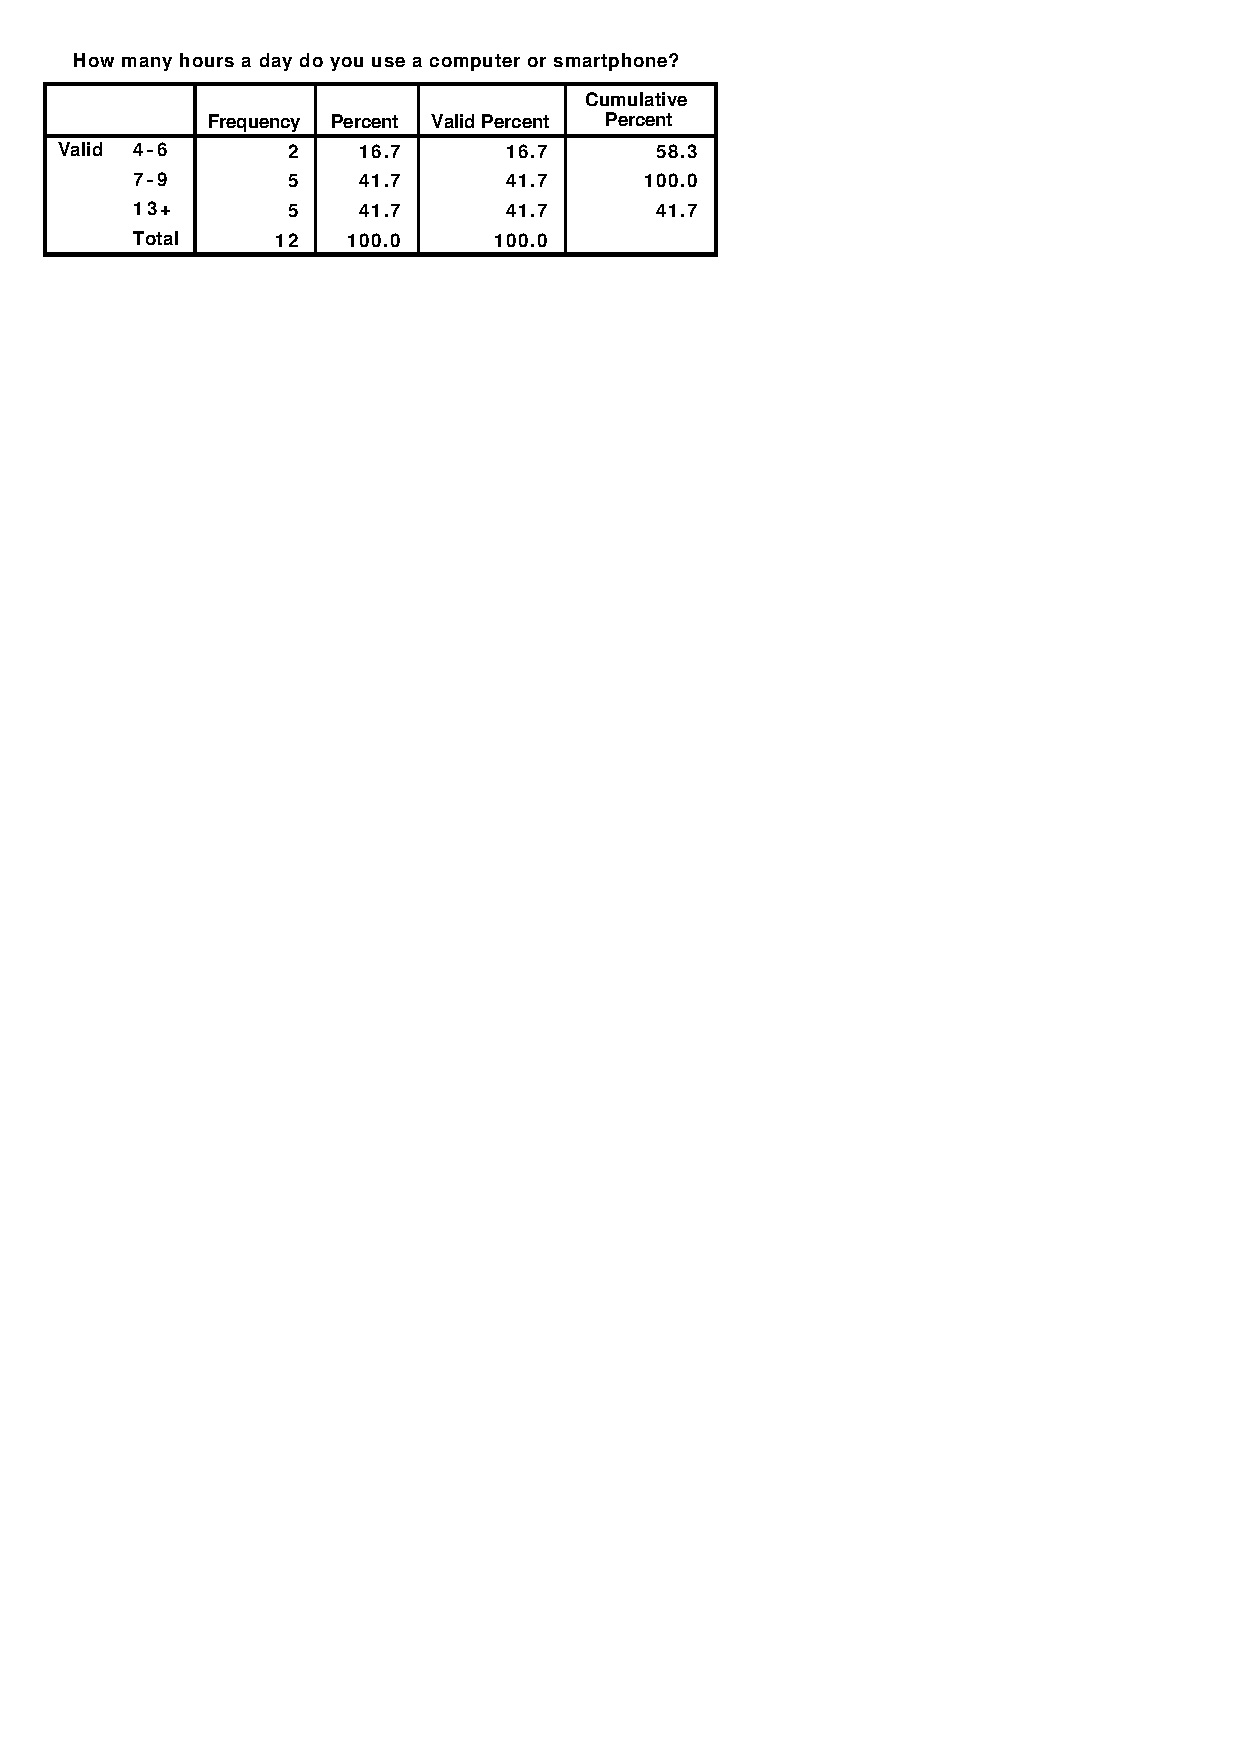
\includegraphics{figures/ComputerHours.pdf}}
\caption{Device usage by participant}
\label{fig:partic_computerHours}
\end{table}

\begin{table}[ht]
\centerline{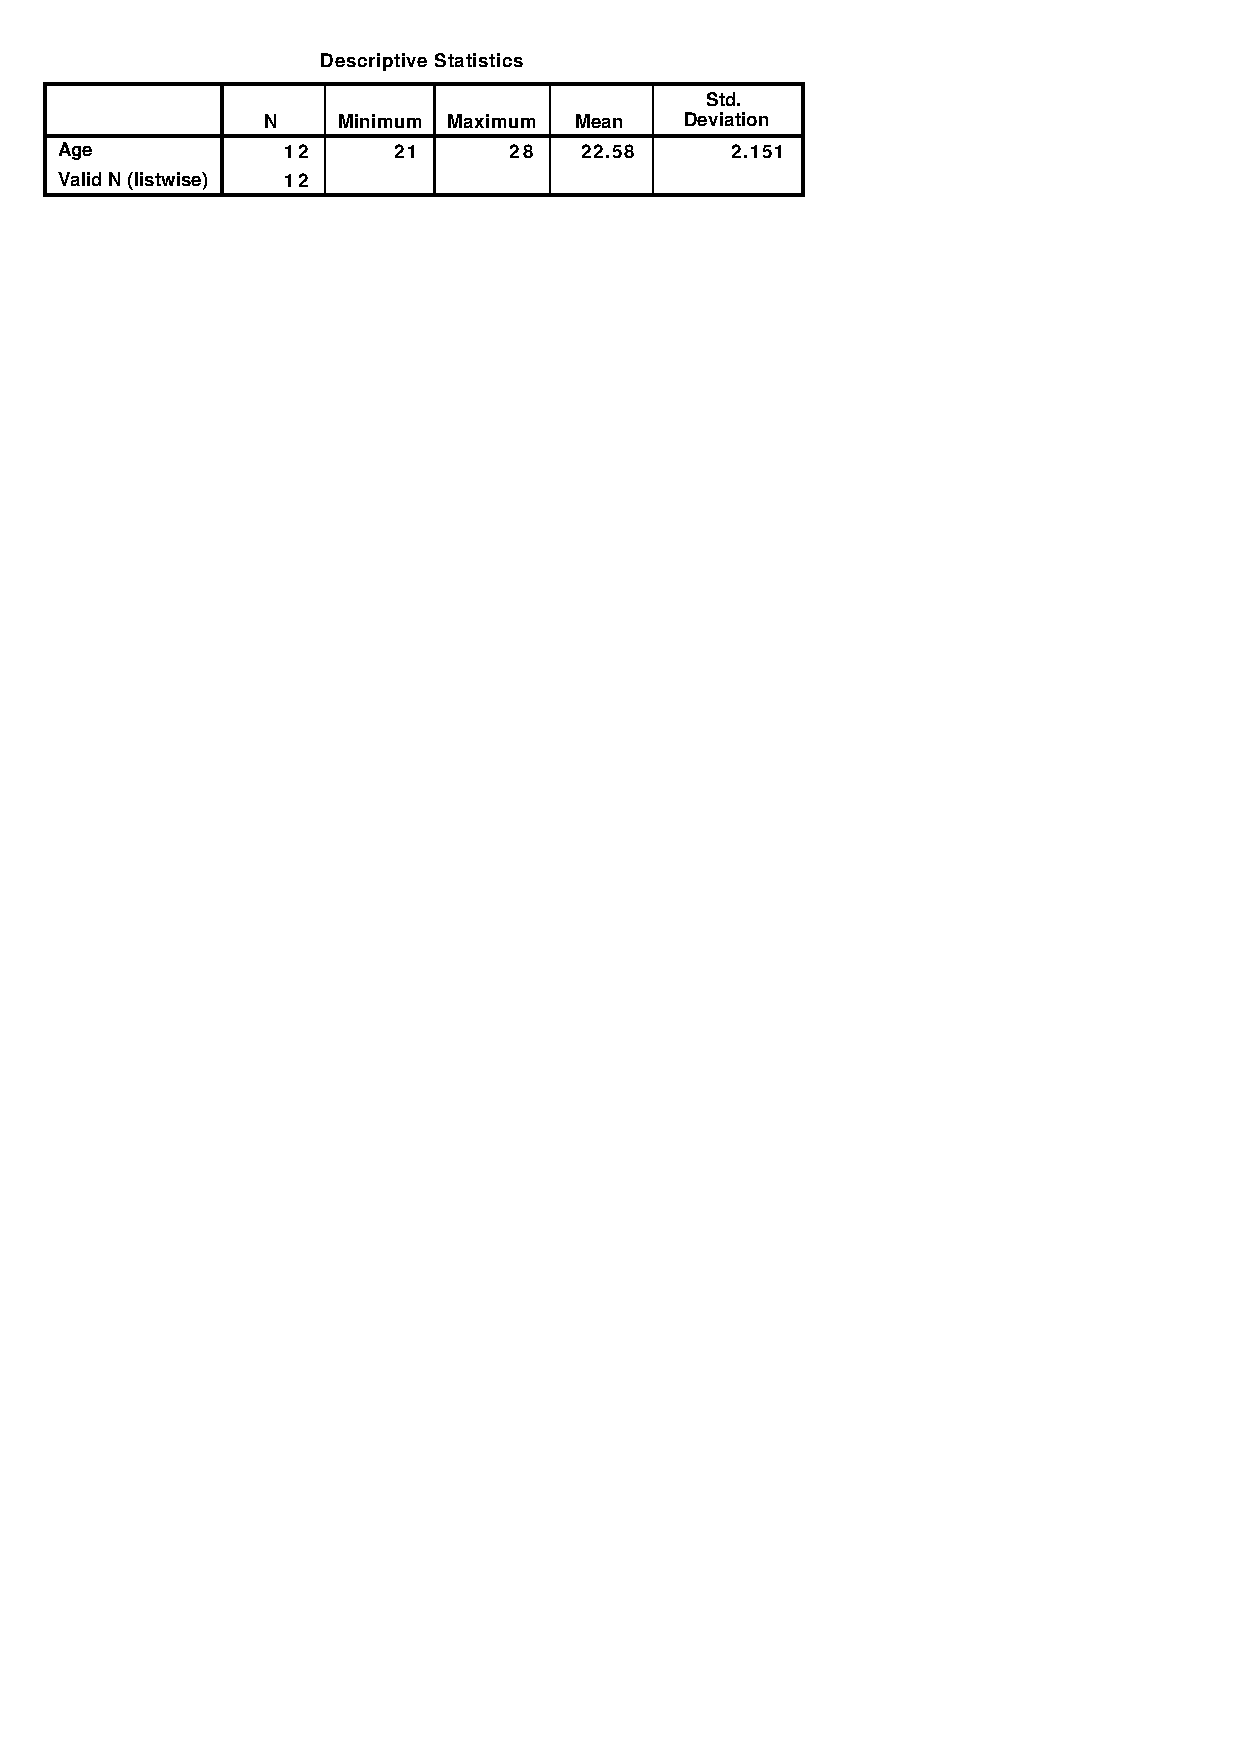
\includegraphics{figures/Age.pdf}}
\caption{Age of participant}
\label{fig:partic_age}
\end{table}

\begin{table}[ht]
\centerline{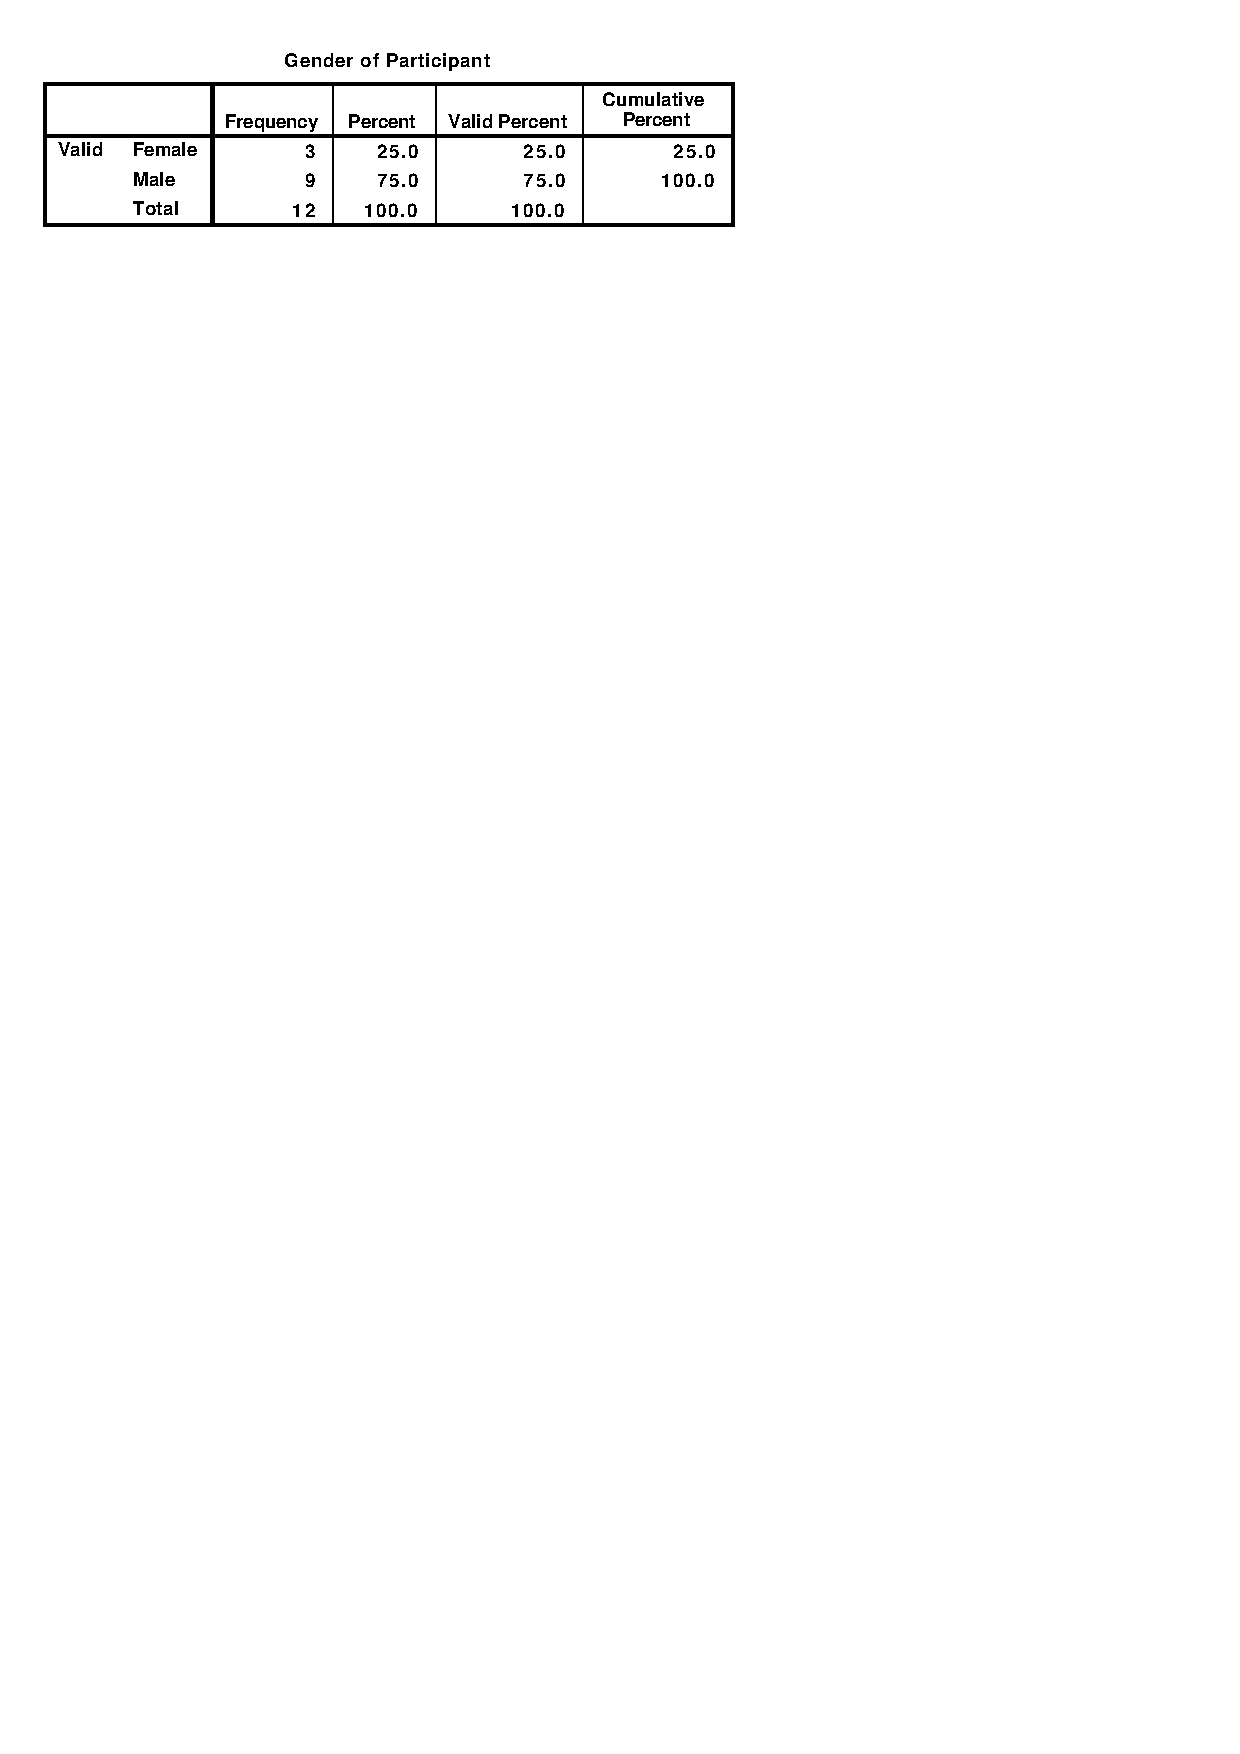
\includegraphics{figures/Gender.pdf}}
\caption{Gender of participant}
\label{fig:partic_gender}
\end{table}

\begin{table}[ht]
\centerline{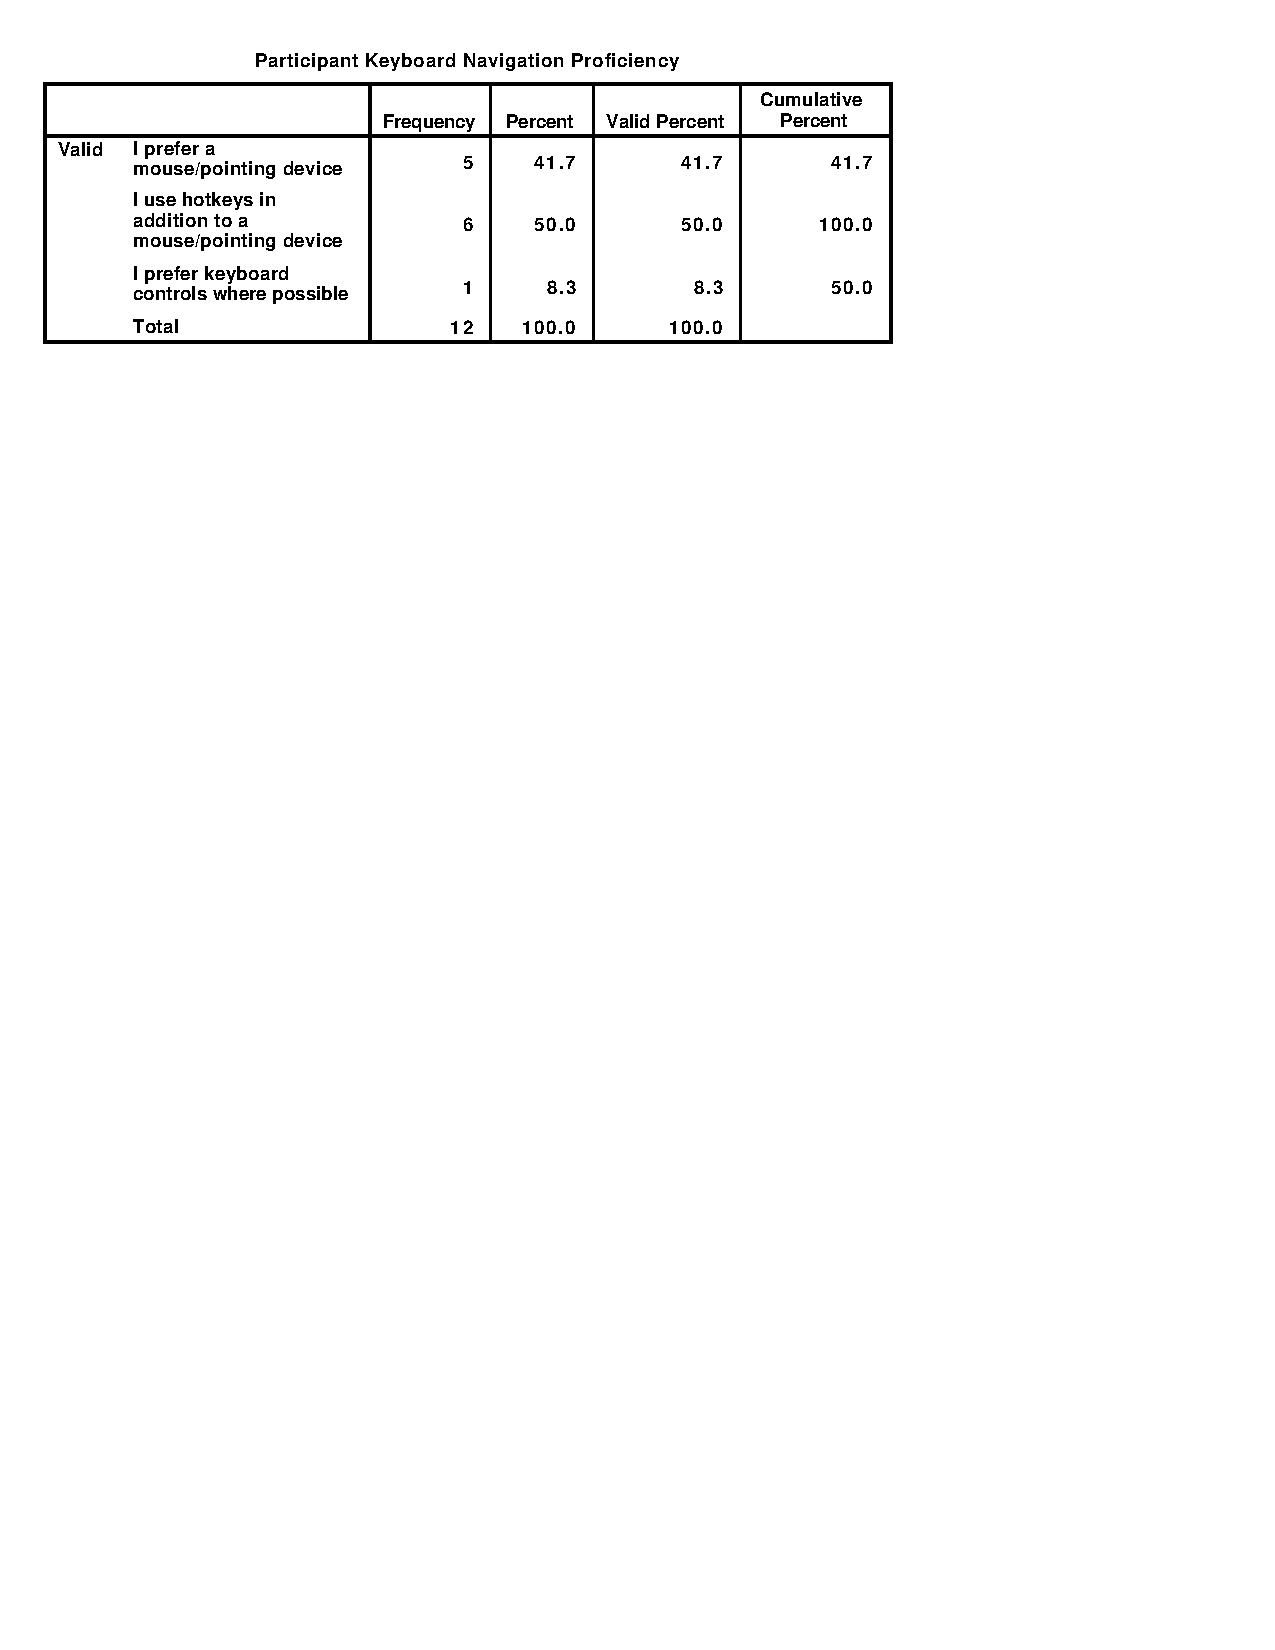
\includegraphics{figures/Proficiency.pdf}}
\label{fig:partic_proficiency}
\medskip
\small
Participants were asked to pick which of these sentiments they identified best with. The statements attempted to describe a proficiency scale for keyboard usage:
\begin{enumerate}
\item I need a mouse/pointing device
\item I prefer a mouse/pointing device
\item I use hotkeys in addition to a mouse/pointing device
\item I prefer keyboard controls where possible
\item I strongly prefer full keyboard support
\end{enumerate}
Votes were cast only for the middle descriptors, 2--4.
\caption{Keyboard Navigation Proficiency of Participants}

\end{table}

\begin{table}[ht]
\centerline{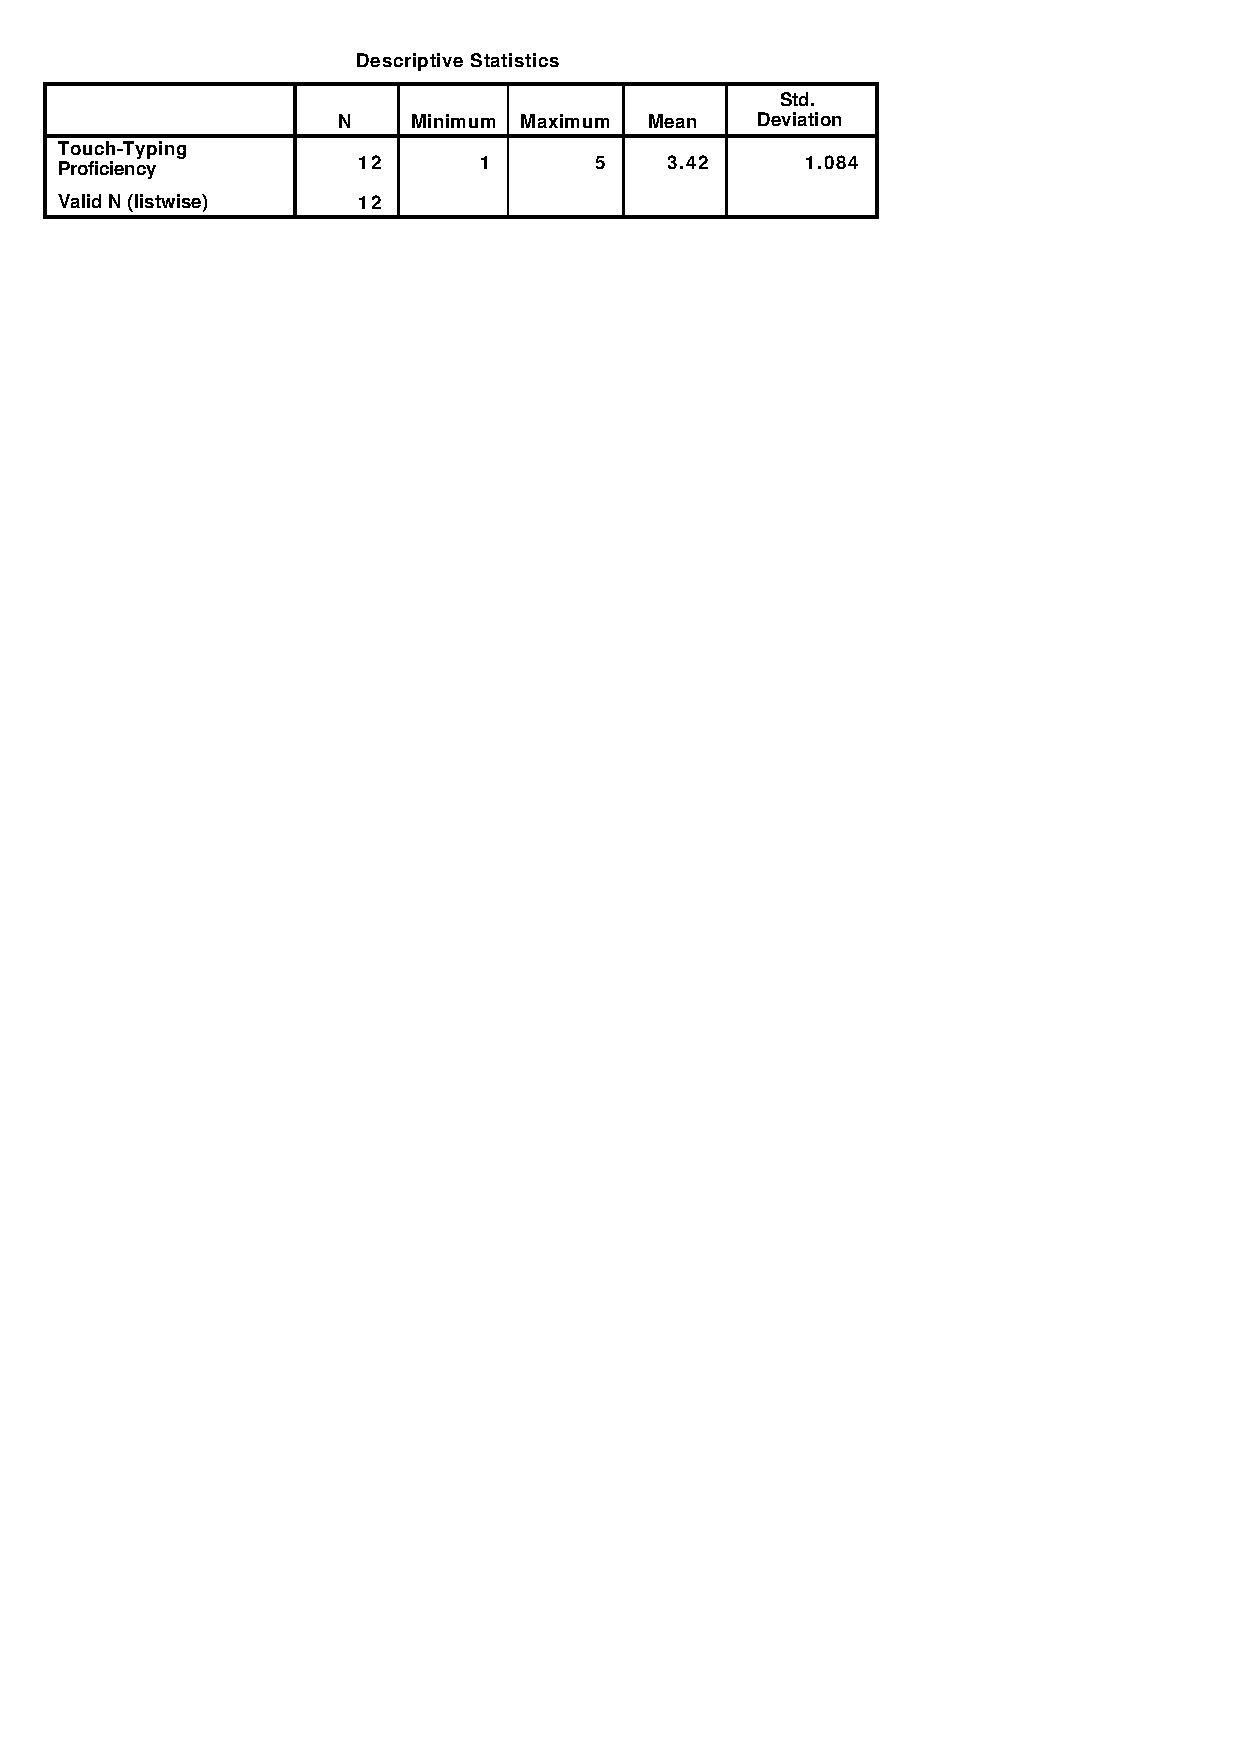
\includegraphics{figures/TouchTyping.pdf}}
\label{fig:partic_ttype}
\medskip
\small
Touch-typing proficiency was rated on a five-point scale ranging from the sentiment `I look at every key before pressing' to `I always type without even a reference glance at the keyboard'.
\caption{Touch-Typing Proficiency of Participants}
\end{table}

%\FloatBarrier

\newcommand{\anumero}{{\fontfamily{cmr}\selectfont\textnumero}}

\begin{table}[ht]
\newcounter{ahref}
\newcommand{\studyhref}{\stepcounter{ahref}\arabic{ahref}}
\begin{tabularx}{\textwidth}{l|X}
\hline\hline %inserts double horizontal lines 
Task \anumero & URL \\ [0.5ex] % inserts table 
\hline 
\studyhref & \url{https://www.halifax-online.co.uk/personal/logon/login.jsp} \\
\studyhref & \url{https://www.kickstarter.com/signup?ref=nav} \\
\studyhref & \url{http://www.bbc.co.uk/} \\
\studyhref & \url{http://www.bath.ac.uk/library/subjects/comp-sci/} \\
\studyhref & \url{http://www.youtube.com/} \\
\studyhref & \url{http://www.amazon.co.uk/s/ref=nb_sb_noss_2?url=search-alias\%3Daps&field-keywords=pillow&rh=i\%3Aaps\%2Ck\%3Apillow} \\
\studyhref & \url{http://www.megatokyo.com/} \\
\studyhref & \url{http://en.wikipedia.org/wiki/Computer} \\
\hline %inserts single line 
\end{tabularx}
\caption{URLs used in tasks (full study)}
\label{fig:fullStudyURLs}
\end{table}

\newcommand*\rot{\rotatebox{90}}
\newcommand{\psize}{1.5cm}
\newcommand{\reasonable}{\rot{(1= Reasonable, 5=Unreasonable)}}

\begin{table}[ht]
\begin{tabular}{|p{\psize}*{8}{|p{\psize}}|}
\hline\hline %inserts double horizontal lines 
\rot{Participant \anumero}	&	\rot{Which system did you prefer using?}	&	\rot{How easy was it to point using Tabbing?}	&	\rot{How was the amount of keypressing}~\rot{required in Tabbing?}~\reasonable	&	\rot{How easy was it to point using CX?}	&	\rot{How was the amount of keypressing}~\rot{required in CX?}~\reasonable	&	\rot{How easy was it to point using CX+F?}	&	\rot{How was the amount of keypressing}~\rot{required in CX+F?}~\reasonable	\\ [0.5ex]
\hline 
1	&	CX+F	&	2	&	5	&	4	&	2	&	5	&	1	\\
2	&	CX	&	2	&	5	&	4	&	1	&	4	&	1	\\
3	&	CX	&	1	&	5	&	5	&	2	&	5	&	1	\\
4	&	CX+F	&	1	&	5	&	3	&	3	&	4	&	2	\\
5	&	CX+F	&	1	&	5	&	5	&	2	&	5	&	1	\\
7	&	CX+F	&	4	&	5	&	4	&	2	&	5	&	2	\\
6	&	CX+F	&	2	&	4	&	4	&	3	&	5	&	2	\\
8	&	CX+F	&	2	&	5	&	4	&	2	&	5	&	1	\\
9	&	CX+F	&	1	&	5	&	4	&	3	&	5	&	2	\\
10	&	CX+F	&	4	&	4	&	4	&	3	&	5	&	2	\\
11	&	CX+F	&	2	&	4	&	4	&	1	&	5	&	1	\\
12	&	CX+F	&	3	&	5	&	5	&	1	&	4	&	1	\\
\hline %inserts single line 
\end{tabular}
\caption{Post-experiment questionnaire responses of Quantitative Study participants}
Ratings were all on a five-point scale, 1--5.
\label{fig:quantpost}
\end{table}

%\begin{table}[ht]
%\renewcommand{\arraystretch}{1.5}
\LTXtable{\textwidth}{figures/Quantitative_PostFeedbackTable.tex}
%\caption{(Continued) Post-experiment questionnaire responses of Quantitative Study participants}
%\label{fig:quantpost_feedback}
%\end{table}

% \begin{tabularx}{\textwidth}{X|X}
% \hline\hline %inserts double horizontal lines 
%Task \anumero & URL \\ [0.5ex] % inserts table 
% \hline
% \studyhref & \url{https://www.halifax-online.co.uk/personal/logon/login.jsp} \\
% \studyhref & \url{https://www.kickstarter.com/signup?ref=nav} \\
% \studyhref & \url{http://www.bbc.co.uk/} \\
% \studyhref & \url{http://www.bath.ac.uk/library/subjects/comp-sci/} \\
% \studyhref & \url{http://www.youtube.com/} \\
% \studyhref & \url{http://www.amazon.co.uk/s/ref=nb_sb_noss_2?url=search-alias%3Daps&field-keywords=pillow&rh=i%3Aaps%2Ck%3Apillow} \\
% \studyhref & \url{http://www.megatokyo.com/} \\
% \studyhref & \url{http://en.wikipedia.org/wiki/Computer} \\
% \hline %inserts single line 
% \end{tabularx}

\end{document}
